% This is a template for Ph.D. dissertations in the UCI format.
% 
% All fonts, including those for sub- and superscripts, must be 10
% points or larger.  Recommended sizes are 14-point for chapter
% headings, 12-point for the main body of text and figure/table
% titles, and 10-point for footnotes, sub- and super-scripts, and text
% in figures and tables.
%
% Notes: Add short title to figures, sections, via square brackets,
% e.g. \section[short]{long}.
%
%\documentclass[12pt,fleqn]{ucithesis} % Orig
\documentclass[12pt]{ucithesis} % CDN - centered equations by default? are they supposed to be left justified?
% A few common packages
\usepackage{amsmath}
\usepackage{amssymb} % CDN added, didn't have mathbb command without it
\usepackage{amsthm}
\usepackage{array}
\usepackage{graphicx}
\usepackage{natbib}
\usepackage{relsize}
\usepackage[titletoc]{appendix}

% Some other useful packages
\usepackage{caption}
\usepackage{subcaption}  % \begin{subfigure}...\end{subfigure} within figure
\usepackage{multirow}
\usepackage{tabularx}
%\usepackage[backend=bibtex,sorting=none]{biblatex} % CDN added
% Uncomment the following to attempt to enforce Type 1 or TrueType 
% fonts. ProQuest does not want the type 3 fonts used by default as
% of Dec. 2019 - see 
% https://support.proquest.com/articledetail?id=kA01W000000k9o2SAA . 
% If you are unable to embed fonts such as 'Zapf Dingbats' or 
% 'Symbol', try using raster images (.jpg or .png) instead of vector 
%images (.pdf or .eps).
% \usepackage[T1]{fontenc} 

% plainpages=false fixes the "duplicate ignored" error with page counters
% Set pdfborder to 0 0 0 to disable colored borders around PDF hyperlinks
\usepackage[plainpages=false,pdfborder={0 0 0}]{hyperref}


% Uncomment the following line to use the algorithm package,
% which provides an algorithm environment similar to figure and table
% ("\begin{algorithm}...\end{algorithm}"). A list of algorithms will
% automatically be added in the preliminary pages. Note that you
% probably want a package for the actual code to go with this (e.g.,
% algorithmic).
%\usepackage{algorithm}

% Uncomment the following line to enable Unicode support. This will allow you
% to enter non-ASCII characters (such as accented characters) directly without
% having to use LaTeX's awkward escape syntax (e.g., \'{e})
% NOTE: You may have to install the ucs.sty package for this to work. See:
% http://www.unruh.de/DniQ/latex/unicode/
%\usepackage[utf8x]{inputenc}

% Uncomment the following to avoid "widowing", where page breaks cause
% single lines of paragraphs to float onto the next page (this is not
% a UCI requirement but more of an aesthetic choice).
%\widowpenalty=10000
%\clubpenalty=10000

% Modify or extend these at will.
\newtheorem{theorem}{\textsc{Theorem}}[chapter]
\newtheorem{definition}{\textsc{Definition}}[chapter]
\newtheorem{example}{\textsc{Example}}[chapter]
%%%%% CDN added commands
\newcommand{\state}{\ensuremath{\mathbf{x}}}
\newcommand{\xut}{\ensuremath{\mathbf{x}_{\mathrm{UT}}}}
\newcommand{\xl}{\ensuremath{\mathbf{x}_{\mathrm{lon}}}}
\newcommand{\control}{\ensuremath{\mathbf{u}}}
\newcommand{\ur}{\ensuremath{u_{\mathrm{ref}}}}
\newcommand{\State}{\ensuremath{\mathbf{X}}}
\newcommand{\Control}{\ensuremath{\mathbf{U}}}
\newcommand{\param}{\ensuremath{\mathbf{p}}}
\newcommand{\Param}{\ensuremath{\mathbf{P}}}
\newcommand{\E}[1]{\mathbb{E}\left[#1\right]}
\newcommand{\V}[1]{\mathbb{V}[#1]}
\newcommand{\EUT}[1]{\sum_{i=0}^{2n}\left[#1\right]}
\newcommand{\mean}{\mathbf{m}}
\newcommand{\cov}{C}
\newcommand{\std}{S}
\newcommand{\rtg}{R}
\newcommand{\y}{\ensuremath{\mathbf{y}}}
\newcommand{\dynamics}{\mathbf{f}}
\newcommand\bigzero{\makebox(0,0){\text{\huge0}}}
\newcommand{\normal}{\mathcal{N}}
\newcommand{\trace}{\mathrm{tr}}
\newcommand{\zero}{\mathbf{0}}
\newcommand{\design}{\mathbf{d}}
\newcommand{\dee}{\mathrm{d}}
%\newcommand{\sample}{\ensuremath{\mathbf{z}}}
%\newcommand{\costate}{\mathbf{\lambda}}
%\newcommand{\multiplier}{\mathbf{\nu}}
%\newcommand{\costate}{\mathbf{p}}
%\newcommand{\multiplier}{\mathbf{\lambda}}
%%%%%

% Macros for title, author, abstract, etc.
\thesistitle{Robust Optimal Entry Guidance for Future Mars Landers}

%"Dissertation" for PhD, "Thesis" for master's
\documenttitle{Dissertation}

\degreename{Doctor of Philosophy}

% Use the wording given in the official list of degrees awarded by UCI:
% http://www.rgs.uci.edu/grad/academic/degrees_offered.htm
\degreefield{Mechanical and Aerospace Engineering}

% Your name as it appears on official UCI records.
\authorname{Connor David Noyes}

% Use the full name of each committee member and full title 
% (e.g. Professor/Associate Professor).
\committeechair{Professor Emeritus Kenneth D. Mease}
\othercommitteemembers
{
  Distinguished Professor Tryphon Georgiou \\
  Professor Athanasios Sideris
}

\degreeyear{2021}

\copyrightdeclaration
{
  {\copyright} {\Degreeyear} \Authorname
}

% If you have previously published parts of your manuscript, you must list the
% copyright holders; see Section 3.2 of the UCI Thesis and Dissertation Manual.
% Otherwise, this section may be omitted.
% \prepublishedcopyrightdeclaration
% {
% 	Chapter 4 {\copyright} 2003 Springer-Verlag \\
% 	Portion of Chapter 5 {\copyright} 1999 John Wiley \& Sons, Inc. \\
% 	All other materials {\copyright} {\Degreeyear} \Authorname
% }

% The dedication page is optional
% (comment out to exclude).
\dedications
{ 
  To my father Michael and my mother Diane.
}

\acknowledgments
{
  I would first like to thank my advisor Kenneth D. Mease, whose expertise shaped not only the course of my research, but also my entire career. 
  
  I would like to thank my fellow UCI colleagues, especially Drs. Guangfei Duan, Eric Trumbauer, and Alessandro Bombelli, for many fruitful discussions during our time together.
  
  I am also indebted to my committee members, Professor Sideris and Professor Georgiou, for their review and suggestions. 
  
  I would also like to thank my colleagues at the Jet Propulsion Laboratory for their advice, and for their patience. My experience at JPL profoundly shaped the direction of my research culminating in this dissertation. Special thanks to Joel Benito, whose guidance and mentorship taught me so much in so little time, and whose friendship I am continually grateful for. I am a better engineer for having known you. 
  
  I gratefully acknowledge the Holmes Endowed Fellowship for it financial support. 
  
  Finally, I am immensely grateful to my mother for all her love and support.
  
%  You also need to acknowledge any publishers of your previous
%  work who have given you permission to incorporate that work
%  into your dissertation. See Section 3.2 of the UCI Thesis and
%  Dissertation Manual.)
}


% Some custom commands for your list of publications and software.
\newcommand{\mypubentry}[3]{
  \begin{tabular*}{1\textwidth}{@{\extracolsep{\fill}}p{4.5in}r}
    \textbf{#1} & \textbf{#2} \\ 
    \multicolumn{2}{@{\extracolsep{\fill}}p{.95\textwidth}}{#3}\vspace{6pt} \\
  \end{tabular*}
}
\newcommand{\mysoftentry}[3]{
  \begin{tabular*}{1\textwidth}{@{\extracolsep{\fill}}lr}
    \textbf{#1} & \url{#2} \\
    \multicolumn{2}{@{\extracolsep{\fill}}p{.95\textwidth}}
    {\emph{#3}}\vspace{-6pt} \\
  \end{tabular*}
}

% Include, at minimum, a listing of your degrees and educational
% achievements with dates and the school where the degrees were
% earned. This should include the degree currently being
% attained. Other than that it's mostly up to you what to include here
% and how to format it, below is just an example.
%
% CV is required for PhD theses, but not Master's
% comment out to exclude
\curriculumvitae
{

\textbf{EDUCATION}
  
  \begin{tabular*}{1\textwidth}{@{\extracolsep{\fill}}lr}
    \textbf{Doctor of Philosophy in Aerospace Engineering} & \textbf{2021} \\
    \vspace{6pt}
    University of California & \emph{Irvine, CA} \\
    \textbf{Master of Science in Aerospace Engineering} & \textbf{2013} \\
    \vspace{6pt}
    California Polytechnic State University & \emph{San Luis Obispo, CA} \\
    \textbf{Bachelor of Science in Aerospace Engineering} & \textbf{2014} \\
    \vspace{6pt}
    California Polytechnic State University & \emph{San Luis Obispo, CA} \\
  \end{tabular*}

\vspace{12pt}
\textbf{ENGINEERING EXPERIENCE}

  \begin{tabular*}{1\textwidth}{@{\extracolsep{\fill}}lr}
    \textbf{Graduate Intern} & \textbf{2015} \\
    \vspace{6pt}
    Jet Propulsion Laboratory & \emph{Pasadena, California} \\
  \end{tabular*}
  
  \begin{tabular*}{1\textwidth}{@{\extracolsep{\fill}}lr}
      \textbf{Guidance and Control Engineer} & \textbf{2015-present} \\
      \vspace{6pt}
      Jet Propulsion Laboratory & \emph{Pasadena, California} \\
    \end{tabular*}

\vspace{12pt}
\textbf{RESEARCH EXPERIENCE}

  \begin{tabular*}{1\textwidth}{@{\extracolsep{\fill}}lr}
    \textbf{Graduate Research Assistant} & \textbf{2013--2021} \\
    \vspace{6pt}
    University of California, Irvine & \emph{Irvine, California} \\
  \end{tabular*}

\vspace{12pt}
\textbf{TEACHING EXPERIENCE}

  \begin{tabular*}{1\textwidth}{@{\extracolsep{\fill}}lr}
    \textbf{Teaching Assistant} & \textbf{2013} \\
    \vspace{6pt}
    California Polytechnic State University & \emph{San Luis Obispo, CA} \\
  \end{tabular*}
  \begin{tabular*}{1\textwidth}{@{\extracolsep{\fill}}lr}
    \textbf{Teaching Assistant} & \textbf{2015} \\
    \vspace{6pt}
    University of California & \emph{Irvine, CA} \\
  \end{tabular*}
\pagebreak

\textbf{PUBLICATIONS}

  \mypubentry{Mars Entry Guidance for High Elevation via Robust Optimal Control}{2021}{Journal of Spacecraft and Rockets (Submitted for Review)}

%\vspace{12pt}
%\textbf{REFEREED CONFERENCE PUBLICATIONS}

  \mypubentry{Entry Guidance for Propellant Optimal Powered Descent on Mars}{Aug 2020}{AAS/AIAA Astrodynamics Specialist Conference}
  \mypubentry{A Convex Optimization Approach to Mars Entry Trajectory Updating}{Aug 2018}{AAS/AIAA Astrodynamics Specialist Conference}
  \mypubentry{High Ballistic Coefficient Mars EDL With Supersonic Retropropulsion}{Feb 2017}{AAS Guidance and Control Conference}
  \mypubentry{Sensitivity Analysis and Uncertainty Quantification of a Mars Ascent Vehicle Concept}{Aug 2017}{ASME Verification and Validation Symposium}  
%  \mypubentry{Hybrid propulsion Mars Ascent Vehicle concept flight performance analysis}{Sep 2017}{IEEE Aerospace Conference}
%  \mypubentry{Mars Ascent Vehicle Model Simulation}{Aug 2016}{AIAA/AAS Astrodynamics Specialist Conference}


}

% The abstract was previously limited to a maximum of 350 words, 
% but the UCI manual at https://etd.lib.uci.edu/electronic/td2e#2.2.1.
% currently does not indicate that there is any word limit for the abstract
\thesisabstract
{
  Mars landings at higher elevations than achieved to date are desired for scientific pursuits. The phases of atmospheric flight are entry, descent, and landing. The research reported here concerns the guidance for the entry phase. We distinguish between the current generation of Mars landers, defined by its continued reliance on Viking-era space technology, and future missions, such as those carrying humans, characterized by significantly higher entry masses and landing ellipse requirements on the order of 100 m, roughly two orders of magnitude smaller than the current generation.
  
  To support higher elevation landing, entry guidance must deliver the entry vehicle to the required altitude with the required horizontal accuracy at the end of the entry phase. The state-of-the-practice entry guidance cannot both raise the final altitude and achieve the required horizontal accuracy at the end of the entry phase. By formalizing the entry guidance objectives as a robust optimal control problem, we seek both to increase the final altitude and to improve the horizontal accuracy. In this approach, we consider only the longitudinal motion and investigate the feasibility of determining a reference trajectory that, in closed-loop reference-trajectory-based guidance, will yield the robust performance required for higher elevation landing. To address robustness, the state variables and uncertain parameters in the entry dynamics are treated as random variables using the unscented transformation to approximate their means and variances and state the performance index in terms of these statistics. Differential dynamic programming is used to solve the robust optimal control problem. Case studies of two different classes of entry vehicle in the current generation demonstrate both the robust performance of the longitudinal entry guidance and the computational feasibility of the design method.
  
  One technology hypothesized to be enabling for landing high mass (and therefore high ballistic coefficient) future missions is supersonic retropropulsion. In the latter part of this dissertation we consider the role of entry guidance in missions where powered descent follows the entry phase directly, without an intermediate parachute deceleration prior to ignition of the retropropulsion. In parachute-based architectures, Mars entry guidance algorithms are judged on their ability to control range errors while reaching the safe parachute deployment set. In contrast, in chuteless missions where pinpoint landing is achieved via powered descent, we posit that performance will instead be based on the required propellant to land the vehicle.   
  A predictor-corrector algorithm, designed to minimize the predicted propellant, is presented. Feasible solutions to the powered descent problem are used to define the entry guidance target set. By computing and storing a mapping from ignition states in the target set to propellant required, the entry guidance algorithm maintains a predicted ignition state that varies over time as various perturbations alter the reachable set of the vehicle. The guidance algorithm updates the bank profile in order to track the propellant optimal reachable state. Simulation results are presented for a hypothetical vehicle with a ballistic coefficient approximately double that of Mars 2020. 
}


%%% Local Variables: ***
%%% mode: latex ***
%%% TeX-master: "thesis.tex" ***
%%% End: ***


% Add PDF document info fields
\hypersetup{
	pdftitle={\Thesistitle},
	pdfauthor={\Authorname},
	pdfsubject={\Degreefield},
}


% Uncomment the following to have numbered subsubsections (by default
% numbering goes only to subsections).
%\setcounter{secnumdepth}{4}



% Set this to only select a subset of the includes directives below.
% Very handy to speed up compilation if you're working on a certain
% part of your thesis. It conserves page numbers, references, etc.
% even for non-included files.
%\includeonly{chapter1,chapter2,chapter3,chapter4}
%\includeonly{chapter5}

\begin{document}

% Preliminary pages are always loaded (TOC, CV, etc.)
\preliminarypages

\parindent 2em

% Include the different components of your thesis, in separate files.
% Using \include allows you to set \includeonly above.
\chapter{Introduction}

% Mars entry problem - mission requirements and future stuff

% State of practice - MSL/M2020

% Covariance reduction based entry guidance - also discussion of sensivity based approaches and comparison work. Also terminology: robust OCP versus optim under unc versus...

% Introduction to my approach? 
% State the specific objectives of my research 

NASA has successfully landed five rovers on Mars to date, including the Mars 2020 rover Perseverance. Each of these missions chose low elevation targets between -1 and -4 km relative to the Mars areoid surface, commonly referred to as MOLA, after the instrument that was used to map Mars' topography. The thin Martian atmosphere makes aerodynamic deceleration ineffective except at lower altitudes where the atmosphere is denser. Coupled with the increasing entry mass required to deliver larger, more capable rovers to the surface, this makes high elevation landing on Mars a challenging problem. Nevertheless, targets above 0 km MOLA, like Terra Sirenum in the Southern Highlands, are motivated by scientific interest \cite{MarsWater}. In order for descent and landing operations to have sufficient timeline margin \cite{BraunMarsEDL,MSL_EDL2} when targeting such elevations, the entry phase must be terminated at a sufficiently high altitude.
%The entry phase may be terminated at a fixed velocity \cite{MSL_EDL2}, at a fixed downrange distance \cite{TriggerComparison2020}, or by a more complex function of the vehicle state \cite{LuAdaptiveEDL}. 
%Increasing altitude at a terminal entry state allows the vehicle to target landing sites at higher elevations, which are motivated by reasons of scientific interest, by increasing the time available for subsequent descent and landing operations, which is particularly important in high ballistic coefficient vehicles. 
In addition to terminal entry altitude, guidance designers must also consider additional objectives, such as reducing the size of the landing footprint. Often these multiple objectives are competing, as for example was the case on the Mars Science Laboratory (MSL) mission, where the entry guidance designers noted that targeting landing site elevations above -1 km MOLA would incur a larger landing ellipse \cite{MSL_EDL2}. 
Future missions, including sample return \cite{MSR} and manned, will place even greater emphasis on robust performance than the current generation, such as pinpoint landing requirements \cite{EvolvableMars}. 

%The state-of-the-practice for Mars entry guidance is represented by Mars 2020, which inherited its entry guidance architecture from MSL \cite{M2020_EDL}. 
%One change from MSL is that Mars 2020 initiated parachute deployment based on a range trigger rather than a velocity trigger \cite{TriggerComparison2020}. 
%MSL and Mars 2020 both utilized the entry terminal point controller (ETPC) \cite{MSL_EDL, M2020_EDL}, a modified version of the Apollo second phase guidance \cite{MSL_EDL2}.
The state-of-the-practice for Mars entry guidance, used on MSL and Mars 2020, is a modified version of the Apollo second phase guidance \cite{MSL_EDL2} called the entry terminal point controller (ETPC). 
The three phases of the ETPC are prebank, range control, and heading alignment. In the prebank phase, there is no guidance, but the vehicle is rotated to the expected initial bank angle for the start of the range control phase.
Range control begins when the vehicle-sensed drag acceleration exceeds a threshold value, and steers the vehicle to the correct downrange distance. This range control affects the longitudinal motion; separate lateral guidance operates during range control to command bank reversals when a measure of the crossrange to the target exceeds the deadband threshold, which is a quadratic function of velocity. At a specified velocity, the guidance switches from range control to heading alignment, during which the bank angle is commanded to reduce the crossrange error.

%TODO: Discuss possibility to handoff to SRP or something other than HeadingAlign/Parameter

The guidance design method used on these latest Mars entry vehicles \cite{MSL_EDL2,M2020_EDL} can be divided into two steps. The first step is to design a reference bank profile and compute the corresponding reference trajectory via open-loop simulation. The reference bank angle profile is specified by a small number of parameters, a modification from the original Apollo algorithm, which assumed a constant bank angle reference profile. This change allows for more flexibility in trajectory design, including enabling higher parachute deploy altitudes \cite{MSL_EDL2}.
In the second step, closed-loop performance using the reference trajectory and bank angle is evaluated under off-nominal conditions. A number of stress trajectories are simulated in closed-loop using the reference trajectory, ETPC gains, and heading alignment guidance to estimate off-nominal performance prior to Monte Carlo simulation \cite{MSL_EDL2}. The results are judged based on the vehicle state at parachute deployment. The free parameters of the guidance algorithm, including the overcontrol gain and heading alignment gain, are then tuned until the performance is satisfactory. If the necessary performance cannot be achieved through tuning, the reference trajectory is changed and the process is repeated. 

In this dissertation, we present an entry guidance law and the method for designing it. Compared with MSL and Mars 2020, the entry guidance objectives are the same, but the means of achieving the objectives and the design method are different. Like the MSL range controller, our guidance law modulates the vertical lift via the bank angle using reference-trajectory-based feedback control to reduce range and altitude dispersions and achieve high altitude, at the initial point of terminal descent which is the point of parachute deployment in the case of MSL and Mars 2020.  The differences in our approach are: (1) to minimize range and altitude dispersions and achieve high altitude, the reference trajectory and bank angle are solutions of a multi-objective robust optimal control problem for the closed-loop dynamics, (2) to address robustness, the state variables and uncertain parameters in the entry dynamics are treated as random variables, using the unscented transformation to approximate their means and variances, and state the performance index in terms of these statistics, (3) rather than a reference bank angle profile determined by a few parameters, a more general piecewise constant reference bank angle profile is considered, and (4) our feedback control law is a constant matrix multiplying the state vector. 
With this design approach, we aim to achieve better performance and avoid the many iterations of the two-step approach, involving 100s or 1,000s of reference trajectories \cite{MSL_EDL2}, used for MSL and Mars 2020. Monte Carlo simulation is only used post-design to validate and further characterize the guidance performance.
%TODO: Remove constant matrix claim above? Maybe not since we're optimizing the constants now 

Uncertainty is quantified using the unscented transformation (UT) \cite{UT1997}, allowing both means and standard deviations of key variables to be considered in the objective function of the optimal control problem, thereby formally addressing robust performance. The UT is a deterministic sampling-based method that propagates a set of sample points through the nonlinear dynamics and reconstructs the mean and covariance from the transformed samples. These sample trajectories allow us to estimate closed-loop guidance performance without Monte Carlo simulation, and thus serve a purpose similar to the MSL stress cases. The UT facilitates a computationally feasible approach to reference bank profile design accounting for uncertainty in a single step, rather than the MSL two-step process.

We demonstrate that, with a reformulation of the objective function, the robust optimal control problem can be solved using differential dynamic programming (DDP) \cite{DDP}, a shooting method originally devised to solve unconstrained nonlinear optimal control problems that has since seen numerous extensions, including to constrained problems \cite{DDP_ControlLimited,HDDP1,HDDP2,DDP_NonlinearConstraints,DDP_InteriorPoint}, and stochastic problems \cite{iLQG, DDP_Stochastic, ozaki_UT,ozaki2020tube}. 
Starting from the control-limited DDP algorithm \cite{DDP_ControlLimited}, we examine a iterated Linear-Quadratic-like simplification \cite{iLQG} that enables solution of large-scale optimal control problems. Next, we extend the algorithm to jointly optimize the static feedback gains along with the reference control.

% TODO: Talk about related work 
%Due to the interest in high elevation landings, guidance algorithms designed to maximize altitude at parachute deploy have been studied using optimal control theory 
%\cite{AltitudeOptimization,AltitudeOptimizationIndirect}. Reference \cite{GuangfeiDissertation} proposed an optimization-based onboard trajectory planning method based on a low-order parametrization designed to achieve high altitude at parachute deploy.
%Typically these papers consider predictive guidance and use parametrizations of the bank angle designed to yield high altitudes. 

% Refences with notes:
% AltitudeUnderUncertainty
% MarsEntryDesensitized % linearized but closed-loop with fixed gain. No consideration of saturation 
% EntryOUU % Does not use linearization, also doesnt solve in a conventional way, maybe remove?
% TrajectoryDesensitization % Desensitized like seywald and kumar, is it entry applied?
% EntryOUUThesis1 % Earth EDL, focuses on footprint computation, only considers open-loop in the reentry problem, and did not conduct monte carlo to confirm
% EntryOUUThesis2 % LQR, minimum control effort objective which stays away from the bounds, angle of attack as control variable. Does perform Monte Carlo(s) to validate improvement. 

Throughout this dissertation, we refer to optimal control formulations that weight a nominal (or mean) optimization objective with minimization of covariance terms as robust optimal control. The nomenclature in the literature also sometimes refer to such problems as uncertain optimal control \cite{PhelpsUncertainOCP}, optimal control under uncertainty. Due to the close relationship between the sensitivity matrix (also called the state transition matrix) and the covariance matrix, we also include desensitized optimal control \cite{Desensitized,TrajectoryDesensitization} under the umbrella of robust optimal control. 
Approaches to entry guidance based on robust optimal control have been studied in \cite{AltitudeUnderUncertainty, EntryOUUThesis1, EntryOUUThesis2, MarsEntryDesensitized, EntryOUU}. Reference~\cite{EntryOUUThesis1} explored the relationship between covariance reduction and sensitivity reduction, and ultimately recommended the covariance formulation for several reasons, including smaller problem size due to the symmetry of the covariance matrix, the ability to incorporate measurements, and simpler formulation and interpretation of variances compared to elements of the sensitivity matrix.

The works most closely related to our approach are Ref.~\cite{AltitudeUnderUncertainty}, where the objective was to maximize a function of the mean and standard deviation of altitude, and Ref.~\cite{MarsEntryDesensitized}, where the objective was to maximize terminal altitude while penalizing sensitivity terms related to variations in the initial state. Compared to Ref.~\cite{AltitudeUnderUncertainty}, our work differs by considering a multi-objective formulation that includes a downrange performance objective rather than strictly focusing on altitude, by considering closed-loop dynamics instead of open-loop, and by using the unscented transform instead of linear covariance propagation. Similarly, Ref.~\cite{MarsEntryDesensitized} also employed linear covariance propagation, but did consider closed-loop performance with fixed feedback gains. Their method made use of sensitivities, rather than statistics, in order to increase robustness to off-nominal situations. Additionally, a single penalty factor was applied to all terminal state sensitivities, including flight path angle. In contrast, we penalize only altitude and downrange deviations, and use a separate penalty factor for each component. An additional difference is that we consider parametric uncertainty in the equations of motion rather than solely uncertainty in the initial state. 

\begin{figure}[h!]
	\centering
	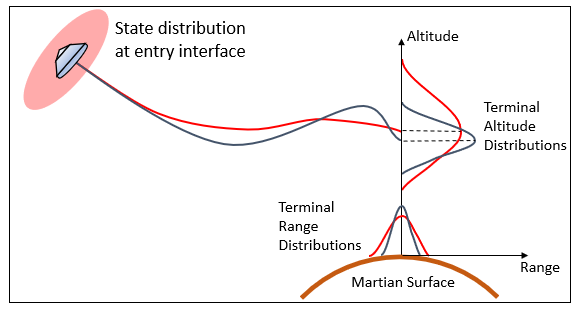
\includegraphics[width=1\textwidth]{Images/RobustTrajectoryOptimization}
	\caption{Comparison of UQ methods in an closed-loop scenario}
	\label{Fig:RobustTrajectoryOpt}
\end{figure}
%The specific objective of this dissertation are to design an entry guidance with the same computational complexity as the state-of-the-practice guidance algorithm while providing superior performance. 

%\section{Dissertation Organization}
This remainder of this dissertation is organized as follows: \\
chapter two discusses the dynamics and models used to describe entry trajectories\\
chapter three describes the entry guidance problem, especially target condition(s)\\
chapter four outlines the guidance strategy, including posing the problem as a ROCP. Gain optimization (or selection) as well. \\
chapter five gives an algorithm based on constrained DDP/SLQ to solve the ROCP; Also UQ and reformulations; demonstration of open-loop vs closed loop necessity of UT \\
chapter six presents the assessment conditions (simulation details, Monte Carlo) Maybe UT-alpha choice should be discussed here?\\
chapter seven presents an assessment of the guidance algorithm. Choice of alpha parameter. Problems with joint optimization as well (UT cov almost zero but MC cov bad) \\
chapter eight concludes the dissertation \\

chapter details two extensions to the DDP algorithm - an augmented lagrangian method for enforcing terminal constraints and a method for optimizing (constant) parameters, such as the feedback gains (lateral corridor params? probably not due to differentiable req) and the initial flight path angle. The gain optimization in particular is important because of the issue with joint optimization of time-varying gains. 

%%% Local Variables: ***
%%% mode: latex ***
%%% TeX-master: "thesis.tex" ***
%%% End: ***

\chapter{Entry Guidance Concepts}
% High level ideas, feedback concepts. Target conditions, current missions vs future. PHASES - prebank, phase 2 (range control),phase 3 heading alignment 

\section{Entry Terminal Point Controller}
The state-of-the-practice for Mars entry guidance, used on MSL and Mars 2020, is a modified version of the Apollo command module entry guidance \cite{MSL_EDL2} called the entry terminal point controller (ETPC). 
The three phases of the ETPC are prebank, range control, and heading alignment. In the prebank phase, there is no guidance, but the vehicle is rotated to the expected initial bank angle for the start of the range control phase.
The range control guidance begins when the sensed drag deceleration exceeds a threshold value, and consists of longitudinal guidance and lateral guidance. Longitudinal guidance modulates the bank angle magnitude to control the range flown, and reduce range dispersions at parachute deployment. Lateral guidance operates concurrently with longitudinal guidance during range control to command bank reversals when a measure of the crossrange to the target exceeds the deadband threshold, which is a quadratic function of velocity. At a specified velocity, the guidance switches from range control to heading alignment, during which the bank angle is commanded to reduce the crossrange error. During heading alignment, the bank angle magnitude is restricted to $30^{\circ}$. This ensures that most of the lift vector is opposite gravity, which results in increased parachute deploy altitude.

For MSL, the entry guidance requirements were 

As its name implies, the purpose of the longitudinal range control is to reduce range errors. Lateral guidance indirectly manages crossrange error during range control, while heading alignment reduces crossrange errors until the sequence leading to parachute deploy is initiated. Thus in the design for MSL, achieving sufficient terminal altitude is accomplished primarily by the choice of the reference trajectory, and numerical simulations were performed to show the range control guidance did not result in lower parachute deploy altitude. 

%The ETPC, as a whole, met the requirements. The components of the approach include the reference trajectory, which fully determines the range control gains, the overcontrol gain operating on range errors, the parameters defining the lateral deadband controlling reversals, and the heading alignment gain. 
%Reversals 
 
%The longitudinal range control guidance uses linear gains computed by the adjoint equations to find a neighboring optimal path that terminates at the same range as the reference trajectory. 

In this dissertation, we propose an alternative to the longitudinal guidance operating during the range control phase. However, because our alternative guidance does not focus exclusively on range, we prefer to refer to the phases by their ordering: first phase is the unguided prebank phase, second phase guidance for MSL and Mars 2020 was range control guidance, and third phase guidance was heading alignment for MSL and Mars 2020, and alternative third phase guidance has been proposed. 

%while the MSL guidance achieves the stated goals (landing footprint, deployment within safe parachute deployment conditions, sufficient timeline)

\section{Entry Guidance Review}
While the ETPC represents the current guidance approach, many alternative entry guidance algorithms have been proposed. There are many ways that algorithms can be characterized and categorized. One popular delineation is between methods that utilize a pre-planned reference trajectory, and those that do not. In the first category are explicit reference tracking approaches in which a feedback law attempts to keep the vehicle state close to the reference state. Many nonlinear control techniques, such as nonlinear model predictive control~\cite{JoelController} and sliding mode control, have been applied to reference tracking guidance. In the latter category are computational approaches, including predictor-corrector guidance~\cite{EntryPredictCorrect}, and convex optimization~\cite{MaxCrossrangeConvexLu,ConvexEntryGuidance}. These methods have higher computational complexity and are highly model dependent.

The advantages of reference-based solutions include designing the reference trajectory before flight, allowing for intensive computations not suitable for in-flight operations. Reference trajectory-based approaches also have some degree of model independence~\cite{joel_dissertation}.

Many entry guidance algorithms blur the line between these approaches. For instance, the ETPC does make use of a reference trajectory, but not does track it directly. Instead, the reference trajectory is used to determine sensitivities, called influence coefficients, that allow the guidance to steer the vehicle along a neighboring path that ends at the same range at a fixed velocity. Because the ETPC makes a prediction of the terminal range and corrects based on the predicted error, it is sometimes called an analytical predictor-corrector. 

%Along the same (blurred) lines, methods that replan a reference trajectory onboard
\section{Entry Guidance Problem}
%(landing footprint, deployment within safe parachute deployment conditions, sufficient timeline)
As the discussion of MSL highlighted, there are several requirements that entry guidance must be able to meet. 
The vehicle must be delivered to safe parachute deployment conditions, generally given as acceptable ranges of dynamic pressure and Mach number, and the deployment must occur high enough to provide timeline margin for terminal descent. The parachute deploy range dispersion limit is flowed back from the landing footprint requirement. MSL determined that the entry phase had to be terminated within 10 km of the parachute deploy target to achieve the desired touchdown ellipse requirement of 25 x 20 km. 

Thus, broadly speaking, the goals are to achieve high terminal altitude and accurate terminal range. 
%Constraints - g-load, heating (handled through selection of mean FPA), and parachute. How are we handling chute? Velocity implies, to an extent, certain mach range. 

\subsection{Entry Phase Termination}
%Termination of the entry phase
Generally speaking, the entry phase of Mars EDL terminates when the sequence leading to parachute deployment begins. For MSL, this sequence was the vehicle reached a fixed velocity \cite{MSL_EDL2}. Mars 2020 instead at a fixed downrange distance \cite{TriggerComparison2020}. Future missions, especially those intending to land without the use of a parachute, may consider a different function of the vehicle state \cite{LuAdaptiveEDL,NoyesSRP}. 
We consider the entry guidance problem is to balance the vertical lift of the vehicle to steer it to the target location at the terminal velocity, and with sufficient altitude for subsequent landing operations. 

Noting that despite using different triggers to terminate the entry phase, MSL and Mars 2020 used the same design process involving parametrizing a reference control profile that terminates at a fixed velocity. Then, in simulations, the appropriate trigger is used. The choice of trigger has a strong impact on the terminal distribution. Naturally, triggering based on the onboard estimate velocity reduces the velocity spread down to approximately the spread in velocity knowledge error. Similarly, a range trigger will naturally minimize the range variations at the trigger point, but will result in larger velocity spreads (though the spread in Mach number is not as large due to wind correlations!\cite{TriggerComparison2020}). In the event of a different trigger, such as one designed to reduce the propellant consumption required to land at the target location, we assume that a similar process can used. For example, the vehicle would carry a fixed amount of propellant
%A key assumption is that reducing the range error at chute deployment translates to a smaller landed footprint. 
% 

Throughout this dissertation we assume the entry phase is triggered based on velocity using the terminal velocity associated with a parachute based landing, corresponding approximately (because Mach also depends on altitude) to deployment at Mach 2. 
%However, this is not the only possibility. We can, for example, target the velocity at which third phase guidance, such as heading alignment \cite{MSL_EDL2} or final position alignment \cite{GuangfeiDissertation}, begins. 

%Discussion of parachute conditions that we aren't modeling in this phase. The parachute conditions could be included in the assessment conditions. Discussion of parachute-free possibilities? 


% The topic of this section is to discuss the actual entry guidance requirements and problem. Not necessarily to pose the robust OCP (?)

%The robust optimal guidance problem is to determine the reference control $u_{\mathrm{ref}}$ that minimizes the cost functional
%\begin{align}
%	J(x,u) = -\E{h} + w_h\sigma_h + w_s\sigma_s \label{eq:cost:mayer}
%\end{align}
%subject to the dynamics
%\begin{align}
%	\dot{\state}(t,\param) = \mathbf{f}(\state(t,\param), u(t), \param)
%\end{align}
%with the initial conditions $\state(0,\param) = \state_0(\param)$, the terminal constraint $v(t_f,\param)=v_f$, and the control constraint $u_{\min}\le u_{\mathrm{ref}}(t)\le u_{\max}\,\forall\,t\in[0,t_f]$. Let $\Omega$ be the space of stochastic parameters with probability density function $\mu(\param)$. The expectation and standard deviations are computed with respect to the uncertain parameters, i.e.,  $\E{F(\state,\param)} = \int_{\Omega}\,F(\state,\param)\mu(\param)\,\mathrm{d}\param$ and $\sigma^2_{F(\state,\param)} = \int_{\Omega}\,\left(F(\state,\param)-\E{F(\state,\param)}\right)^2\mu(\param)\,\mathrm{d}\param$.
%\section{}


%%% Local Variables: ***
%%% mode: latex ***
%%% TeX-master: "thesis.tex" ***
%%% End: ***

\chapter{Entry Vehicle and Environment Models}\label{Ch:Models}
In this chapter we present the models of the entry vehicle and Mars environment used in the development and assessment of the entry guidance algorithm.
Vectors are denoted by boldface and are assumed to be columns. $(\cdot)^T$ denotes the transpose of a vector. 
The trace of a square matrix is the sum of its diagonal entries and is denoted $\trace(\cdot)$.   
%The gradient of a scalar function with respect to a vector is a row vector, i.e., $\mathbf{v}^T = \frac{\partial h(\y)}{\partial\y}$. 
The mean, or expected value, of a random variable, $\y$, is denoted by $\E{\y}=\bar{\y}$, and its covariance matrix by $\V{\y} = \cov_{\y}$. 
The standard deviation of a scalar random variable $y$ is $\sigma_{y} \triangleq \sqrt{\V{y}}$. A normal distribution with mean $\bar{\mathbf{y}}$ and covariance matrix $\cov_{\mathbf{y}}$ is $\normal(\bar{\mathbf{y}}, \cov_{\mathbf{y}})$.

\section{Three Degree-of-Freedom Dynamics Model}
The three degree-of-freedom translational dynamics for a Mars entry vehicle are defined relative to a Mars-fixed coordinate frame. In this three degree-of-freedom modeling, we have assumed that the velocity frame and the body frame are aligned, and do not consider the vehicle attitude.
% Talk about different independent variables, reduced longitudinal state vector 
The dynamics of an entry vehicle in an atmosphere are modeled by Vinh's equations \cite{VinhDyanmics}:
\begin{align}
	\dot{r} &= v\sin\gamma \label{Eq:dynamics:radius:time}\\
	\dot{\theta} &= \frac{v}{r}\frac{\cos\gamma\cos\psi}{\cos\phi} \\
	\dot{\phi} &= \frac{v}{r}\cos\gamma\sin\psi \\
	\dot{v} &= -D - g\sin\gamma \\ 
	\dot{\gamma} &= \frac{L}{v}\cos\sigma + \left(\frac{v}{r}-\frac{g}{v}\right)\cos\gamma + C_{\gamma}\\
	\dot{\psi} &= -\frac{L}{v\cos\gamma}\sin\sigma - \frac{v}{r}\cos\gamma\cos\psi\tan\phi + C_{\psi}\label{Eq:dynamics:heading:time}
\end{align}
where $r$ is the distance from the center of Mars to the center of mass of the entry vehicle, and $\theta$ and $\phi$ are latitude and longitude, respectively; the velocity vector is defined by the magnitude of the planet-relative velocity, $v$, the flight path angle $\gamma$, and the heading angle angle $\psi$, defined counterclockwise from East. The bank angle, $ \sigma $, is the clockwise rotation angle between the lift vector and the vertical plane containing the velocity vector; thus $\sigma=0$ corresponds to the full lift-up orientation. 
The magnitude of the gravitational acceleration is $g=\mu/r^2$, and $\mu=42,828\, \mathrm{km}^3/\mathrm{s}^2$ is the gravitational constant of Mars. Mars is assumed to be a sphere with planet radius $r_p=3396.2$ km, and the altitude above the surface is $h=r-r_p$. The aerodynamic accelerations are 
\begin{align}
		L &= \frac{1}{2}\rho v^2 \frac{S}{m}C_D \label{Eq:lift_accel}\\
		D &= \frac{1}{2}\rho v^2 \frac{S}{m}C_L \label{Eq:drag_accel}
\end{align}
where $\rho$ is the atmospheric density of Mars, $S$ is the vehicle surface area, and $m$ is the vehicle mass.  The Coriolis terms, $ C_{\gamma} $ and $ C_{\psi} $, are
\begin{align}
	\begin{split}
		C_{\gamma} &= 2\omega_p\cos\psi\cos\phi \\
		C_{\psi} &= 2\omega_p(\tan\gamma\sin\psi\cos\phi-\sin\phi)
	\end{split}
\end{align}
with planet rotation rate $\omega_p=7.08\times10^-5$ rad/s. 

Separation of the longitudinal and lateral guidance has proven effective in the state-of-the-practice approach, and we follow this when developing the robust optimal entry guidance algorithm. In place of the coordinates $(\theta,\,\phi)$, the distance along the great circle arc defined by the vehicle heading is substituted. Ignoring the offset between the great circle azimuth and the instantaneous vehicle heading, this distance is computed by integrating
\begin{align}
	\dot{s} = v\cos\gamma
\end{align}
and the longitudinal state vector is $\state_{\mathrm{lon}} = [r,\,s,\,v,\,\gamma]^T$. An important quantity related to $s$ is range-to-go. For a terminal target range, $s_{\mathrm{target}}$, the range-to-go is $\rtg=s_{\mathrm{target}}-s$. During flight, the target distance is fixed, and thus $\dot{\rtg}=-\dot{s}$.
The longitudinal dynamics are 
\begin{align}
	\dot{h} &= v\sin\gamma \label{Eq:dynamics:altitude:time}\\
	\dot{s} &= v\cos\gamma \\
	\dot{v} &= -D - g\sin\gamma \label{Eq:dynamics_velocity:time}\\ 
	\dot{\gamma} &= \frac{L}{V}\cos\sigma + \left(\frac{v}{h+r_p}-\frac{g}{v}\right)\cos\gamma \label{Eq:dynamics:fpa:time}
\end{align}
%The dynamics of the longitudinal state vector with respect to the planet-relative velocity are 
%\begin{align}
%	h' &= \frac{v\sin\gamma}{-D - g\sin\gamma} \label{Eq:dynamics:altitude:vel}\\
%	s' &= \frac{v\cos\gamma}{-D - g\sin\gamma} \\
%	\gamma' &= \frac{\frac{L}{V}\cos\sigma + \left(\frac{v}{h+r_p}-\frac{g}{v}\right)\cos\gamma}{-D - g\sin\gamma} \label{Eq:dynamics:fpa:vel}
%\end{align}

\section{System Models}
% MarsGRAM vs time-varying mean/std model used in optimization process 
\subsection{Nominal Models}
The density of the Martian atmosphere is modeled by an exponential function
\begin{align}
	\rho(h) = \rho_0\exp(-\frac{h}{h_s}) \label{Eq:Density}
\end{align}
where $\rho_0=0.0158\,\mathrm{g}/\mathrm{m}^3$ is the reference density and $h_s=9.354$ km is the scale height. This profile is shown in Fig.~\ref{Fig:DensityNominal}. The speed of sound is also modeled as a function of altitude. 

The vehicle is assumed to be a low lift entry capsule. In the numerical assessment presented in Chapter~\ref{Ch:AssessmentConditions}, the vehicle is in the same class as MSL, with a lift-to-drag ratio $L/D\in[0.24, 0.31]$. A heavier vehicle with a nominal $L/D=0.28$ is considered in Chapter~\ref{Ch:SRL_EDL}. The aerodynamic coefficients are, in general, functions of Mach number and angle of attack. As is common in entry guidance developments, the angle of attack profile is assumed to be a fixed function of Mach number, and thus the coefficients depend solely on Mach number. The nominal aerodynamic coefficient profiles are curve-fitted from 500 MSL profiles~\cite{joel_dissertation}. The nominal coefficients, and their ratio $L/D = C_L/C_D$, are shown for the MSL-class vehicle in Fig.~\ref{Fig:AeroCoeffNominal}.
\begin{figure}[h!]
	\centering
	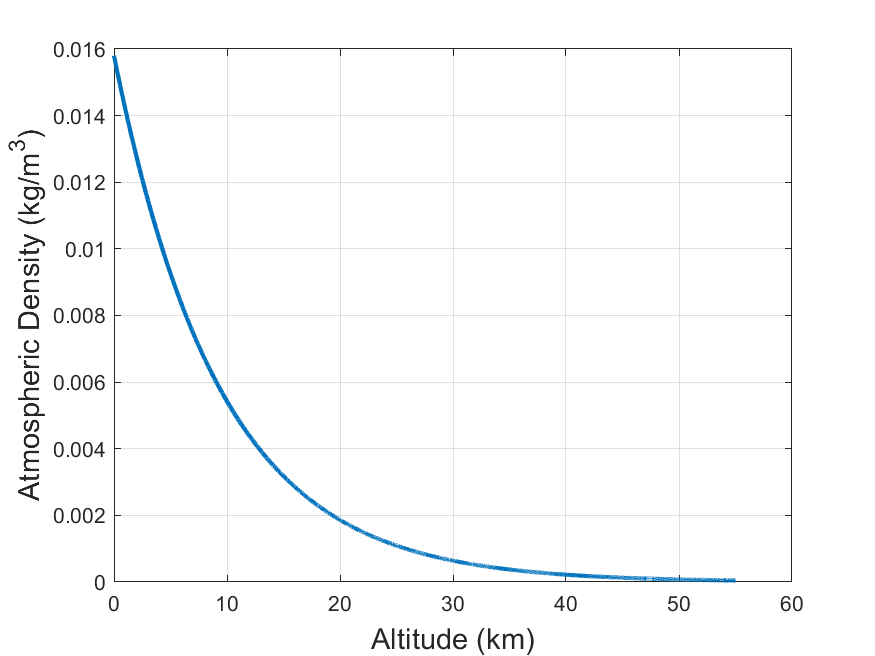
\includegraphics[width=1\textwidth]{Images/DensityNominal}
	\caption{The nominal atmospheric density.}
	\label{Fig:DensityNominal}
\end{figure}
\begin{figure}[h!]
	\centering
	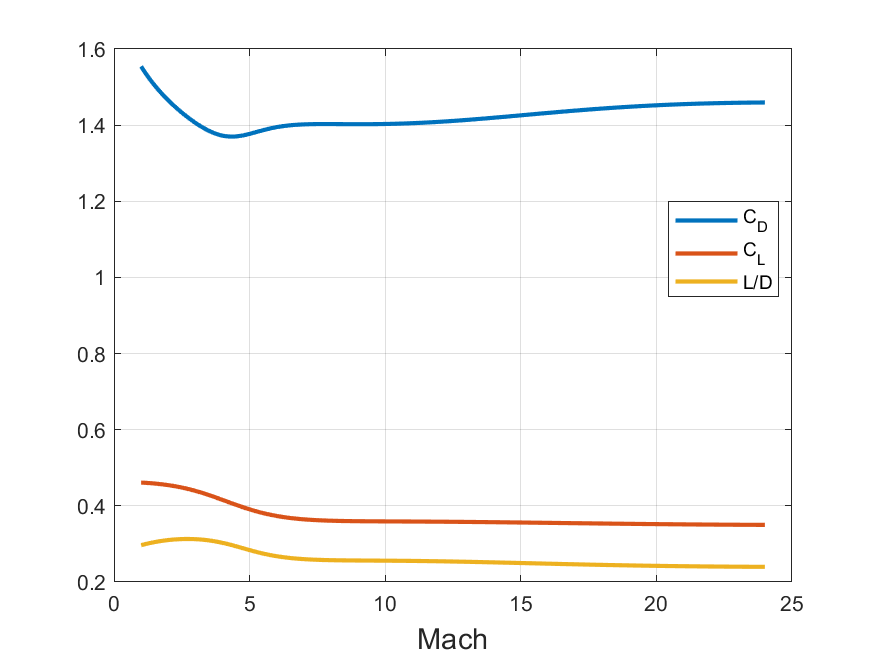
\includegraphics[width=1\textwidth]{Images/CoeffNominal}
	\caption{The nominal aerodynamic coefficients and $L/D$ profile.}
	\label{Fig:AeroCoeffNominal}
\end{figure}

\subsection{Uncertainty Models}
Typically, the uncertain initial state and model parameters are discussed in the context of assessing the guidance algorithm. However, in this dissertation, a key component of the guidance approach is incorporating uncertainty during the reference trajectory design, and thus they are given here. All uncertain variables are assumed to be normally distributed, but we note that the guidance approach developed in this dissertation applies to any distributed parameters with known mean and covariance. 

The approach phase, prior to the entry phase, targets a nominal entry state, but errors in the insertion maneuver and navigated state result in an uncertain entry state
\begin{align}
	\state(t_0, \delta\state_0) &= \bar{\state}_0 + \delta\state_0 \\
	\delta\state_0 &\sim \normal(\mathbf{0}, \cov_{\state_0}) \nonumber
\end{align}

Two key quantities in the study of entry vehicles are the lift-to-drag ratio, $L/D$, and ballistic coefficient, $\beta = \frac{m}{SC_D}$. Often, uncertainty is modeled in these values rather than in the aerodynamic coefficients, $C_L$ and $C_D$. For this reason, it is useful to rewrite Eqs.~(\ref{Eq:lift_accel})-(\ref{Eq:drag_accel}) in terms of these quantities and their uncertainties:
\begin{align}
	\begin{split}
		D &= \frac{1}{2}\frac{\rho}{\beta(1 + f_{\beta})} v^2 \\
		L &= D(\frac{L}{D})(1+f_{\frac{L}{D}})  \label{Eq:aero_accels}
	\end{split}
\end{align}
where $f_i\sim\normal(0, \sigma^2_i)$ are constant fractional offsets from the mean profile.
% i.e., $\delta\beta = \beta f_{\beta}$ and $\delta\frac{L}{D} = \frac{L}{D} f_{\frac{L}{D}}$.

Another key source of uncertainty in the entry dynamics is the atmospheric density model. The deviations are modeled as 
\begin{align}
	\rho(h) = \bar{\rho}(h) + f_{\rho}\delta\rho(h) \label{Eq:DensityUnc}
\end{align}
where $\bar{\rho}(h)$ is given by Eq.~\eqref{Eq:Density}. In Eq.~\eqref{Eq:DensityUnc}, the deviation $\delta\rho(h)$ is free to vary independently from the mean density. Note that this assumes that a constant fraction $f_{\rho}\sim\normal(0, \sigma^2_{\rho})$ of the standard deviation is applied throughout the trajectory. This can be used to bound the altitude-varying, possibly asymmetric density disturbances of models like MarsGRAM~\cite{MarsGRAM2010} or the Mars Climate Database (MCD)~\cite{MarsClimateDB}. See Fig.~\ref{Fig:DensityVariations} for an example where the boundary is determined by 1000 samples from the MCD~\cite{GuangfeiDissertation} and a symmetric model is created to bound the MCD model. Symmetry is required due to the Gaussian uncertainty assumption. 
\begin{figure}[h!]
	\centering
	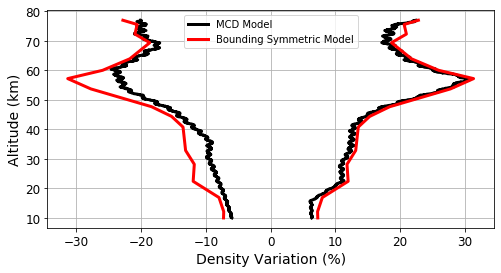
\includegraphics[width=0.9\textwidth]{Images/DensityVariations}
	\caption{Density variations from 1000 Mars Climate Database samples}
	\label{Fig:DensityVariations}
\end{figure} 

Collecting these uncertainties in the vector-valued random variable $\param = [\delta\state_0,\, f_{\frac{L}{D}},\, f_{\beta},\, f_{\rho}]^T$, the uncertain vehicle dynamics are written compactly as
\begin{align}
	\dot{\state}(t,\param) &= \dynamics(\state(t,\param), u(t,\state), \param),\quad
		\state(t_0,\param) = \state_0(\param) \label{Eq:UncertainDynamics}
\end{align}
where $\param \sim \mu = \normal(\mathbf{0},\cov_{\param})$ and 
\begin{align}
	\cov_{\param} = \begin{bmatrix}
		\cov_{\state_0} & & &\bigzero \\ 
		 &\sigma^2_{\frac{L}{D}} \\
		 & & \sigma^2_{\beta} \\
		\bigzero & & & \sigma^2_{\rho}
	\end{bmatrix}
\end{align}
%The domain and probability density function of the state vector vary with time. For this reason, the expected value is taken with respect to $\param$ throughout this dissertation. By the law of the unconscious statistician, 
%\begin{align}
%	\E{x(t,\param)} = \int_{\mathbb{R}^{n_p}}x(t,\param)\mu(\param)\mathrm{d}\param
%\end{align}
Note that, for a given realization of $\param$, the dynamics are a deterministic function of the state and control. A nominal trajectory is defined as one in which $\param=\mathbf{0}$. For nonlinear systems like the entry dynamics, the mean trajectory is not generally equal to the nominal trajectory, except at the initial time. 
The Taylor series of a generic scalar variable, $x(t,\param)$, expanded around $\param=\mathbf{0}$, is 
\begin{align}
	x(t,\param) = x(t,\mathbf{0}) + \Phi_1\param + \frac{1}{2}\param^T\Phi_2\param + \dots
\end{align} 
where $\Phi_i,\,i=1,2,3,\dots$ are the $i^{\mathrm{th}}$ partial derivatives of $x$. 
Truncating the series at second order and taking the expectation yields
\begin{align}
	\E{x(t,\param)} &= \E{x(t,\mathbf{0}) + \Phi_1\param + \frac{1}{2}\param^T\Phi_2\param} \\
	 &= x(t,\mathbf{0}) + \E{\frac{1}{2}\param^T\Phi_2\param}
\end{align}
where the second line follows from the linearity of the expectation operator and $\E{\param} = \mathbf{0}$. This latter fact also means $\cov_{\param} = V[\param] = \E{\param\param^T}$. 
The trace is also a linear function, so the expectation and trace can be swapped, i.e., $\E{\trace(A)} = \trace(\E{A})$. Together with the identity $\param^TA\param = \trace(A\param\param^T)$, we arrive at
\begin{align}
	 	\E{x(t,\param)} &= x(t,\mathbf{0}) + \frac{1}{2}\trace(\Phi_2\cov_{\param}) \label{Eq:TaylorExp}
\end{align}
From Eq.\eqref{Eq:TaylorExp} it can be seen that the nominal trajectory provides a first-order estimate of the mean. 
%We remark that a number of technical conditions on both the function $\dynamics$ (convergence of the Taylor series to the function) and the distribution of the random variable $\param$ (existence of higher moments, strong concentration) are required for the validity of the above Taylor series expansion analysis. However, this result is presented purely for analysis, and the numerical solution method presented later does not make use of it.
%TODO: rewrite this last part, maybe move it up. 



%%% Local Variables: ***
%%% mode: latex ***
%%% TeX-master: "thesis.tex" ***
%%% End: ***

\chapter{Guidance Strategy}\label{Ch:GuidanceStrategy}
In this chapter we present the guidance strategy, which is to pose the guidance problem as a robust optimal control problem. 
The guidance law for longitudinal range control has an affine feedback structure, consisting of a reference vertical $L/D$ profile and a feedback control law, subject to physical- and safety-related constraints. Thus, to design the guidance means to design the reference vertical $L/D$ and corresponding longitudinal reference trajectory, and the feedback gains. 
%
%The physical constraint is that the available lift is limited, so the most vertical lift that can be achieved is with zero bank angle, or $u=\cos\sigma=1$. The lower bound is dependent on the mission and vehicle characteristics. Physics again limits the magnitude to $u=-1$, but it is often prudent to further limit the lower bound due to the low $L/D$ of typical Mars entry vehicles.

\section{Independent Variable}
Following from the assumption that the entry phase is terminated at a fixed velocity, it is essential to use velocity as the independent variable. If time were used, at best we could constrain the mean velocity at the final time to be equal to the terminal velocity, but there would nevertheless be a distribution of final velocities. Using velocity as the independent variable naturally guarantees that the entire distribution of trajectories will terminate at the same velocity.
Redefining $\state_{\mathrm{lon}} = [h,\,s,\,\gamma]^T$ to remove the velocity state variable, the dynamics with respect to velocity, with $ (\cdot)' $ denoting the derivative with respect to velocity, are 
\begin{align}
	\state_{\mathrm{lon}}'(v,\param) &= \dynamics_v(v,\xl(v,\param),u(v),\param) \label{Eq:DynamicsWRTVel}\\
	&= \begin{bmatrix}
		\frac{\dot{h}}{\dot{v}} \\
		\frac{\dot{s}}{\dot{v}} \\
		\frac{\dot{\gamma}}{\dot{v}} 
	\end{bmatrix}
\end{align}
One issue with this choice, however, is that velocity may not be monotonically decreasing from the entry interface because, at high altitudes, $D\approx0$ and so $\dot{v}=-D-g\sin\gamma$ is dominated by the gravity term until the vehicle descends into denser atmosphere. Because the gains used by MSL and M2020 during range control were interpolated as functions of the velocity magnitude, they had to contend with a similar issue.

Recall that MSL and Mars 2020 had a pre-bank phase prior to range control; this phase ended when the magnitude of vehicle sensed drag acceleration exceeded 1.96 m$/\mathrm{s}^2$ \cite{MSL_EDL2}.
With Martian gravity approximately $3.71$ m/s$^2$, this is sufficient drag to ensure monotonicity for $\gamma$ as steep as $-30^{\circ}$, noting that both MSL and Mars 2020 had entry flight path angles around $-15.5^{\circ}$. 

Because drag is a function of both altitude and velocity, the point at which $D$ reaches its threshold value is not at a single velocity for all realizations of $\param$. Thus, we can consider a very similar solution except that pre-bank ends at a fixed velocity rather than a fixed drag magnitude. Denoting this velocity by $v_0$, this value is essentially the highest velocity for which $D(v_0,\state,\param)>D_{\mathrm{threshold}}$ and is driven by the lowest drag scenario (high altitude, low density, high ballistic coefficient). 
Since the entry uncertainties are generally specified at the entry interface and not at the start of range control, an ensemble of points is propagated from the entry interface to $v_0$, and the mean and covariance matrix at this point become the initial state and covariance used in the robust guidance problem. 

%Given $\bar{\state},\cov_{\state}$ at the EI altitude $\sigma_h=0$, simulate $u = \cos\sigma_{\mathrm{pre}}$ to a ``low" velocity, determine $v_0$, and finally compute $\state_0$ and $\cov_{\state_0}$. 


\section{Feedback Control Form}
As a result of considering uncertainty, the state variables are random variables and the goal is to optimize a distribution of trajectories rather than a single trajectory.
In designing the reference trajectory, the effects of feedback control on the distribution are accounted for. Thus the closed-loop control $u$ consists of both a reference control $\ur$, and a feedback control $\delta u$, in contrast to open-loop design methods where $u=\ur$. 
The control law is assumed to be to a saturated linear state feedback 
\begin{align}
	u(v,\state_{\mathrm{lon}}) &= \mathrm{sat}_{[0,1]}\left(\frac{\frac{L}{D})_{\mathrm{ref}}\ur(v)}{\frac{L}{D}} + \delta u(v,\state_{\mathrm{lon}})\right) \label{Eq:Control}\\
	\delta u &= k_D\delta D + k_{\gamma}\delta\gamma + k_s\delta s \label{Eq:Feedback}
\end{align}
%TODO: L/D control, reference Eq.3 in MSL design paper, talk about the "strange" form of the open loop component
where we note that, consistent with state-of-the-practice EDL operations on Mars, drag acceleration has been used as a feedback term in place of altitude. 
%This is due to relationship between drag and $s$,
%\begin{align}
%	s = -\int_{E_0}^{E_f}$\frac{\cos\gamma}{D}\mathrm{d}E \approx -\int_{E_0}^{E_f}$\frac{1}{D}\mathrm{d}E
%\end{align}
In the numerical results presented later, the gains $[k_D, k_{\gamma}, k_s]$ in Eq.~(\ref{Eq:Feedback}) are chosen to be constant values, but they may in general be functions of velocity. 
The MSL and Mars 2020 velocity-dependent gains could be used; they are designed, based on linearized dynamics, to fly a trajectory neighboring the reference which ends with the desired range. Our constant gain feedback control is always driving the perturbed trajectory back to the reference. %We will demonstrate that good guidance performance can be achieved.
The saturation function is defined
\begin{align*}
	\mathrm{sat}_{[a,b]}(x) = \left\{\begin{array}{lc}
		a, &  x < a\\
		x, &  a\le x \le b\\
		b, &  b < x
	\end{array} \right. % The period stops a warning about not closing the left 
\end{align*}
The saturation function is required to ensure that, regardless of the value of the reference control $ \ur $, the feedback control $u(v,\state)$ always satisfies the control limits. Because the control variable is the cosine of an angle, its magnitude must be bounded by one. Due to the low lift capability of current generation Mars entry capsules, it may be prudent to further restrict the vehicle from bank angles that orient the lift vector downward, so in our application we apply
\begin{align}
	0 \le \ur(v) \le 1 \label{Eq:Control_bounds}
\end{align}
which disallows bank angle magnitudes greater than $90^\circ$. Since vertical $L/D$ is equal to $\frac{L}{D}u$, Eq.~\eqref{Eq:Control_bounds} serves the same purpose as the $L/D$ limiter used on MSL and Mars 2020~\cite{MSL_EDL2}. Equation~\eqref{Eq:Control_bounds} limits the reference control, while the saturation function in Eq.~\eqref{Eq:Control} limits the closed-loop control. These bounds need not be equal; ad hoc control margin could be gained by imposing tighter bounds in Eq.~\eqref{Eq:Control_bounds} than in the saturation function, but instead we set them to be equal and allow the optimization process, presented in the following chapter, to determine the robust optimal margin along the trajectory.

The state deviations in Eq.~\eqref{Eq:Feedback} are computed with respect to the reference state at the current velocity, e.g., $\delta D(v) = D(v) - D_{\mathrm{ref}}(v)$.
The form of Eq.~\eqref{Eq:Control} may be unfamiliar but notice that when the control is not saturated, Eq.~\eqref{Eq:Control} may be rearranged as
\begin{align}
	\frac{L}{D}u(v,\state_{\mathrm{lon}}) &= \frac{L}{D}_{\mathrm{ref}}\ur(v) + \frac{L}{D}\delta u(v,\state_{\mathrm{lon}}) \label{Eq:Control_rearranged}
\end{align}
Compared with the ETPC (see Eq.~(2) in Ref.~\cite{MSL_EDL2}), the only difference lies only in the feedback terms $\delta u$. Just like the ETPC, the control in Eq.~\eqref{Eq:Control} commands the reference vertical $ L/D $, rather than a reference fraction of the available $ L/D $, which turns out to be a more robust choice in the presence of aerodynamic uncertainty.

\section{Defining the Objective Function}
The first objective is to maximize the mean altitude at the final velocity while minimizing the altitude standard deviation
\begin{equation}
	\max J_h = \bar{h}(v_f) - w_h\sigma_h(v_f) \label{Eq:AltitudeObjective}
\end{equation}
where $w_h\ge0$ is a penalty on the standard deviation. Maximizing Eq.~(\ref{Eq:AltitudeObjective}) for $w_h=0$ results in an optimal mean altitude, while $w_h>0$ maximizes a measure of the low end of the altitude distribution. For example, $w_h=3$ maximizes the 3$\sigma$-low altitude. 

The second objective, consistent with the range control objective, is to minimize the standard deviation of range 
\begin{equation}
	\min J_s = w_s\sigma_s(v_f) \label{Eq:RangeObjective}
\end{equation}
In contrast to Eq.\eqref{Eq:AltitudeObjective}, the mean range is not included in the objective. This is because for altitude, achieving a very tight altitude distribution is not sufficient; the mean altitude must also be high for the low end of the distribution to have sufficient timeline margin. Regardless of the length of the trajectory flown, the goal is to minimize the standard deviation to achieve a tight distribution. While for a given mission the target location on the ground may be fixed, during mission planning the entry point can adjusted to accommodate the optimal trajectory length. 

The overall performance objective is simply the sum of $J_h$ and $J_s$, posed as a minimization problem
\begin{align}
	\min J = -\bar{h}(v_f) + w_h\sigma_h(v_f) + w_s\sigma_s(v_f) \label{Eq:Objective}
\end{align}
Due to the nonlinear dynamics, the state distribution will not remain normally distributed; nevertheless we assume that standard deviations remain an appropriate measure of the spread of the distribution. That is, that a reduction in standard deviation will lead to a tighter distribution regardless of the shape of the distribution. Either variances or standard deviations may be used in Eq.~(\ref{Eq:Objective}). In practice, appropriate choices of the weights can produce equivalent results, but standard deviations are preferred because they are in the same units as the state variables, and allow for more natural interpretations of the weights. An additional consideration is that the square root is not differentiable at zero, but in practice, the terminal standard deviations are never exactly zero. Additionally, a small term $\epsilon<<1$ can be added to safeguard against this issue in the event the terminal covariance matrix is only positive semidefinite.
%, as might be the case at the initial velocity when considering a certain initial state subject to parametric uncertainty. 
%TODO: Could talk about the perspective of nominal + robustness instead of altitude vs range 
%TODO: Discuss the strangeness of defining a reference trajectory by the closed loop mean? Normally, a reference trajectory is created, and the mean is estimated via MC after simulation. 

\section{The Robust Optimal Guidance Problem}\label{Sec:ROGP}
In summary, the robust optimal guidance problem (ROGP) is to determine $u[v_0,v_f]$, parametrized by $\ur(v)$ and $K(v)$, that minimizes
\begin{align}
	&\min J = -\bar{h}(v_f) + w_h\sigma_h(v_f) + w_s\sigma_s(v_f) \nonumber\\
	&\mathrm{subject\, to }\nonumber \\
	&\xl'(v,\param) = \dynamics_v(v, \xl(v,\param), u(v), \param),\quad
	\xl(v_0,\param) = \state_0(\param) \label{Eq:ROGP}\\
	&\param\sim \normal(\mathbf{0},\cov_{\param}) \nonumber\\
	&0 \le \ur(v) \le 1 \quad \forall\,v\in [v_0, v_f] \nonumber
\end{align}
The robust optimal guidance solution consists of the reference control and the reference trajectory, and the feedback gains. The reference trajectory is defined to be the mean trajectory, $\bar{\state}_{\mathrm{lon}}(v)$, rather than the nominal trajectory, $\xl(v,\zero)$. 

The succinct form of Eq.~\eqref{Eq:Objective} perhaps belies the challenging, highly nonlinear nature of the objective functional, which features multiple integrals over the uncertainty space
\begin{align}
	\min J = &-\int_{\mathbb{R}^{n_p}}h(v_f,\param)\mu(\param)\dee\param \nonumber\\
	&+ w_h\left[\int_{\mathbb{R}^{n_p}}\left(h(v_f,\param) - \bar{h}(v_f)\right)^2\mu(\param)\dee\param\right]^{\frac{1}{2}} \\
	&+ w_s\left[\int_{\mathbb{R}^{n_p}}\left(s(v_f,\param) - \bar{s}(v_f)\right)^2\mu(\param)\dee\param\right]^{\frac{1}{2}}\nonumber
\end{align}
where we recall that $\mu = \normal(\mathbf{0},\cov_{\param})$ is the probability density function of $\param$. The following chapter will discuss the use of the unscented transform to form a tractable, finite-dimensional approximation to the objective functional. Part of the motivation behind using the mean state to define the reference trajectory is that, if the unscented transform estimates the mean range accurately, then by using the mean range as the target range, the mean range error should be very nearly zero in the Monte Carlo assessment results. 

%%% Local Variables: ***
%%% mode: latex ***
%%% TeX-master: "thesis.tex" ***
%%% End: ***

\chapter{Solving the Robust Optimal Guidance Problem}\label{Ch:SolutionMethod}
% UT transform to quantify mean/std of key variables
% Reformulation of the problem as a running cost and with a fixed independent variable 
% SLQ version of Differential Dynamic Programming algorithm for large scale solution 
% Analysis of necessary conditions??

Solving the robust optimal guidance problem presents a number of challenges. In this chapter we first discuss our choice of uncertainty quantification method used to compute the mean and standard deviation of key variables. Next we present the differential dynamic programming algorithm used to numerically solve the guidance problem. Finally, we detail several modifications to the problem to make it amenable to solution via DDP.

\section{Uncertainty Quantification}\label{Sec:UQ}
A key issue in solving the robust optimal guidance problem is computing the expected values and standard deviations in the objective functional and feedback terms. Broadly speaking, uncertainty quantification (UQ) methods trade between accuracy and the amount of computation required. For example, linear covariance propagation is one of the most efficient UQ methods for computing the first two probability moments, but its accuracy depends on the nonlinearity of the system dynamics. At the other extreme, Monte Carlo simulation can estimate higher order moments to arbitrary accuracy, but may require a huge number of samples in order to do so. Since UQ will be performed at each optimal control solver iteration, the method chosen must strike a careful balance these two aspects. For very fast but inaccurate methods, the solution may not perform as expected in a higher fidelity UQ, such as Monte Carlo simulation, and the benefit of the approach may be diminished or lost entirely. On the other hand, accurate methods will result in very long solution times. In this work, the unscented transform (UT) \cite{UT1997} is chosen to compute the required statistics. The following subsections review linear covariance and unscented transform methods. Then, via numerical example, we demonstrate that the saturation nonlinearity, introduced by the feedback control formulation Eq.~\eqref{Eq:Control}, is more accurately accounted for using the unscented transform. 

%The UT is preferable to linear covariance propagation in our application because the sigma points, described in a following subsection, are propagated through the full nonlinear, saturated dynamics, and are thus able to capture their effects on the distribution more accurately than linearization.

\subsection{Linear Covariance}
In the linear covariance methodology, the entry dynamics are linearized around a nominal state-control trajectory, and the mean trajectory is assumed to be equal to the nominal trajectory, i.e., $ \E{\state(v,\param)} \approx \state(v,\mathbf{0}) $. Compared with Eq.\eqref{Eq:TaylorExp}, we see this neglects a term related to the product of the covariance matrix and the trajectory curvature. 
The covariance matrix is propagated by integrating the Lyapunov differential equation
\begin{align}
	\dot{\cov}_{\state}(t) &= A(v)\cov_{\state}(v) + \cov_{\state}(v)A^T(v) \\
	A(v) &= \frac{\partial \dynamics_v}{\partial\state}\bigg\rvert_{x(v,\mathbf{0})}
\end{align}
subject to the initial condition $\cov_{\state}(v_0) = \cov_{\state_0}$. Note that the linearization around the nominal trajectory uses dynamics with respect to velocity, Eq.~\eqref{Eq:DynamicsWRTVel}. 
%TODO: clraify the notation, parameters are include in the state vector and thus the derivatives as well. 

\subsection{Unscented Transform}\label{Sub:UT}
The unscented transform is a method to approximate the first two moments of a nonlinear transformation of a probability distribution. Consider a scalar quantity $q\in\mathbb{R}$ resulting from a nonlinear transformation $q = F(\y)$ of a random vector $\y\in\mathbb{R}^n$ with known mean $ \bar{\y} $ and covariance $ \cov_{\y} $. A set of $2n+1$ sigma points and associated weights are computed 
\begin{align*}
	\y_0 &= \bar{\y} \\
	\y_i &=  \bar{\y} + \left(\sqrt{(\alpha+n) \cov_{\y}}\right)_i,\, \,i=1,...,n \\
	\y_{i+n} &=  \bar{\y} - \left(\sqrt{(\alpha+n)\cov_{\y}}\right)_i, \, \,i=1,...,n\\
	w_0 &= \frac{\alpha}{\alpha+n} \\
	w_i &= w_{i+n} = \frac{1}{2(\alpha+n)}, \, \,i=1,...,n
\end{align*}
where $\alpha$ is a scaling parameter, and $\left(\sqrt{(\alpha+n)\cov_{\y}}\right)_i$ is the $i^{\mathrm{th}}$ column of the matrix square root of $(\alpha+n) \cov_{\y}$. The sigma points are then mapped through the transformation
\begin{align}
	q_i = F(\y_i),\;\;i=0,...,2n
\end{align}
and finally, the mean and variance are estimated using the weights and transformed sigma points
\begin{align*}
	\bar{q} &\approx \sum_{i=0}^{2n}w_iq_i\\
	\sigma_{q} &\approx \left(\sum_{i=0}^{2n}w_i\left(q_i - \bar{q}\right)^2\right)^{\frac{1}{2}}
\end{align*}
In our application, $\y=\param$, the nonlinear transformation is the integration of the longitudinal entry dynamics to the terminal velocity, and the quantities of interest are downrange distance and altitude. For a given covariance matrix and a chosen value of $\alpha$, the ensemble of sigma points may be collected into a single extended vector, and the robust guidance problem is now a deterministic problem in the extended state space.
\begin{align}
	X = \begin{pmatrix}
	\state^{(0)}\\
	\vdots\\
	\state^{(2n)}
	\end{pmatrix}
\end{align}
When applying the unscented transform, the scaling parameter $\alpha$ is important in precisely estimating the statistics. For any value of $\alpha$, the sigma point distribution has the same mean and covariance as the initial distribution. Increasing the value of $\alpha$ places the sigma points $\y_i$ further from the nominal sigma point $\y_0$ and reduces their weight. Using a small value of $\alpha$ results in sigma points with only small deviations from the nominal, and for the entry guidance problem in this paper, the effects of the controller and saturation nonlinearity will not be accurately quantified. In our numerical studies, it appears that no single value of $\alpha$ minimizes estimation errors for all control profiles and all quantities of interest. However, it is important to recall that estimating statistics is not the purpose of the proposed trajectory optimization. So long as the reference trajectories designed using the UT confer benefits in Monte Carlo simulation, the UT statistics are sufficiently accurate, as will be demonstrated by the results of the numerical assessment. 

\subsection{Linear Covariance vs Unscented Transform Example}\label{Subsec:UQExample}
In this subsection we present a numerical example demonstrating the shortcoming of linear covariance propagation for our application to closed-loop entry guidance.
We simulate the performance of an MSL class entry vehicle using the feedback control, Eq.~\eqref{Eq:Control}. The example considers a single, non-optimized reference control and trajectory, and two sets of static feedback gains, $K_1=[0,0,0]^T$ and $K_2=[0.0725, -0.025, -0.004]^T$. $K_1$ corresponds to the open-loop case. The ballistic coefficient at the initial velocity is $\beta=120\,\mathrm{kg/m}^3$ and $L/D = 0.24$. The reference control is a linear-in-velocity ramp from 0.35 to 1. Additional details such as initial state and covariance are given in Chapter~\ref{Ch:AssessmentConditions}.
%TODO: finish giving the problem data,  uncertainties,

The terminal statistics are computed with three different UQ methods: linear covariance propagation (LC), unscented transform (UT), and Monte Carlo (MC). While the MC statistics are themselves estimates of the true mean and variance, accurate estimates can be by using a sufficiently large sample size. Thus they are the values against which statistics computed by LC and UT are compared. The UT scaling parameter $\alpha=15$ is used; sensitivity to this parameter is discussed below. Table~\ref{Table:UQCompareOpenLoop} presents the terminal statistics for the results using $K_1$; in this open-loop problem both LC and UT perform well. LC underestimates mean altitude by 1.2 km and altitude standard deviation by 200 m, underestimates mean range by 1 km, and overestimates range standard deviation by 1.1 km. In contrast, the UT overestimates the mean altitude by 160 m, the altitude standard deviation by 65 m, underestimates mean range by 800 m, and overestimates range standard deviation by 180 m. While the UT estimates a better in each variable, the LC estimates could be considered sufficient for the purposes of optimization. 

\begin{table}[h!]
	\centering
	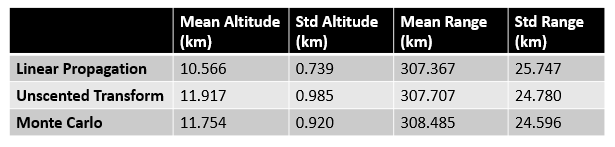
\includegraphics[width=1\textwidth]{Images/UQExample_Open}
	\caption{Comparison of UQ methods in an open-loop scenario}
	\label{Table:UQCompareOpenLoop}
\end{table}
\begin{table}[h!]
	\centering
	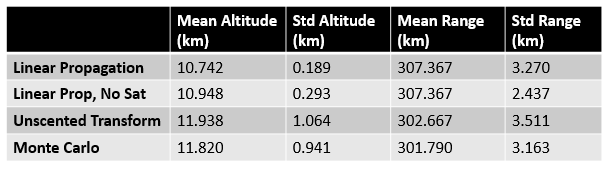
\includegraphics[width=1\textwidth]{Images/UQExample_Closed}
	\caption{Comparison of UQ methods in an closed-loop scenario}
	\label{Table:UQCompareClosedLoop}
\end{table}

Table~\ref{Table:UQCompareClosedLoop} presents the terminal statistics for the results using $K_2$. Linear propagation is listed twice; the first case linearizes the dynamics including the saturated controller defined in Eq.~\eqref{Eq:Control} while the second linearizes the controller without the saturation nonlinearity. In essence, the latter choice assumes the feedback control is not subject to the control limits, and as a result overpredicts the efficacy of the controller, as seen by the large underpredictions of the standard deviation of both altitude and range. Closed-loop robust optimal control was explored using linear sensitivity propagation without considering saturation in \cite{MarsEntryDesensitized}.
Both linearizations once again underpredict the mean altitude substantially. The UT overpredicts the mean range by 900 m and otherwise is once again accurate to within a few hundred meters or less for the remaining statistics. Note that this control profile has significant margin throughout the trajectory except close to the final velocity; in this case control saturation is likely not as significant as for reference control profiles that spend more time at or near the control limits. The UT is expected to produce greater benefits over LC in such scenarios.

\begin{figure}[h!]
	\centering
	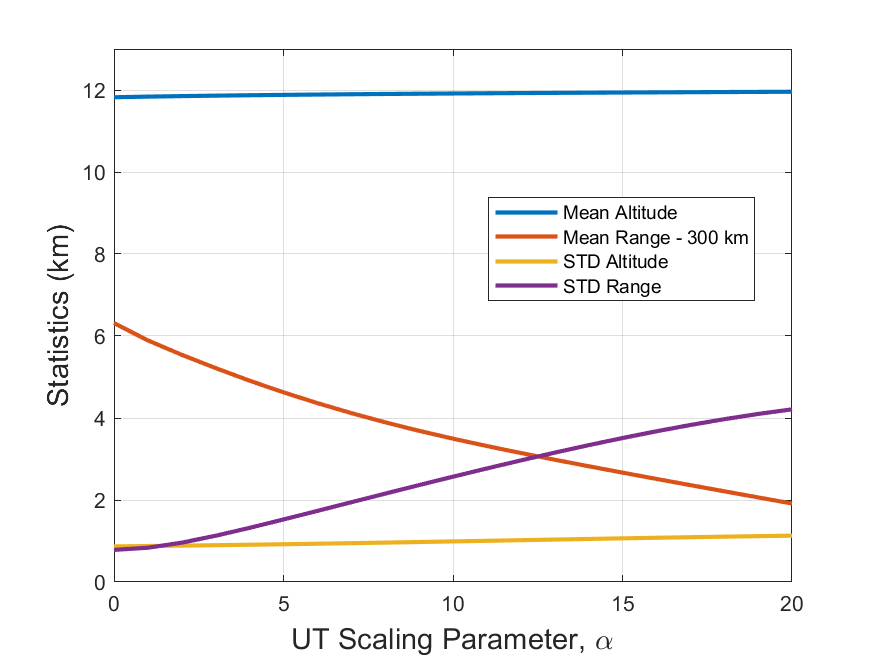
\includegraphics[width=1\textwidth]{Images/AlphaSensitivity}
	\caption{Sensitivity of statistics to the unscented transform scaling parameter}
	\label{Fig:AlphaSensitivity}
\end{figure}

Figure~\ref{Fig:AlphaSensitivity} shows how the UT-estimated means and standard deviations vary with different choices of the scaling parameter. Note that the mean range has been shifted down 300 km to fit it in the same figure. The altitude statistics are quite stable and vary only slightly with $\alpha$, while the effect is much stronger for range. This is a general phenomenon we have observed across numerous control profiles; as a result we recommend selection of $\alpha$ based on range considerations. 
Both the mean range and its standard deviation vary monotonically with $\alpha$. In this example, the mean range error is minimized for $\alpha = 20$, while $\sigma_s$ is approximately optimized for $\alpha = 13$. Our choice $\alpha=15$ strikes a balance between these two. 
While the tuning parameter $\alpha$ is important, we note that in this example the UT estimates of $\bar{h},\,\sigma_h$, and $\bar{s}$ are more accurate than either LC method for all of $\alpha$ values considered, and $\sigma_s$ is better for several values.
This example is meant to motivate our choice of the UT over LC; more detailed examples utilizing optimal solutions are presented in Chapter~\ref{Ch:NumericalAssessment}. 
%TODO: Show control profile, trajectory plots with MC samples, UT points? Or maybe just estimated 3-sigma bounds but might be too messy with three on there Also show a table of the terminal statistics. 

%Sensitivity to $\alpha$  
%Talk about the (weak) dependence on alpha, such that we can choose a single decent value and use it for all of the solutions? 

\section{Differential Dynamic Programming}\label{Sec:DDP}
We begin this section by reviewing the control-limited differential dynamic programming method, proposed in Ref.~\cite{DDP_ControlLimited}, that will be used as the basis for solving the robust optimal guidance problem. The following subsections discuss modifications to the algorithm and the problem formulation that will finally enable the solution of the problem. In the first subsection we present a extension of the algorithm that allows for the joint optimization of static design parameters. The following subsection proposes a simplification that vastly reduces computational time and memory requirements at the expense of lower convergence rate. This simplification is instrumental in solving the large-scale problem. Next, we discuss a reformulation of the performance objective into a Lagrange (or running) cost instead of a Mayer (or terminal) cost. Finally, we present a differentiable approximation to the saturation nonlinearity in the controller, Eq.~\eqref{Eq:Control}. Since DDP requires derivatives of the dynamic equations with respect to the reference control, state variables, and potentially the feedback gains, replacing the non-differentiable saturation function is essential to the numerical solution.

DDP is a trajectory optimization method that iteratively solves for a locally optimal trajectory and control starting from a nominal trajectory and control.

This particular DDP algorithm is formulated in discrete time, so the continuous time dynamics must be discretized. In our numerical examples, Euler integration is used:
\begin{align}
	\state_{i+1} = \mathbf{f}(v, \state_i,\control_i) = \state_i + \state_i'\Delta v \label{Eq:DiscreteDynamics}
\end{align}
A trajectory $\{\State,\Control\}$ is a sequence of controls $ \Control=\{\control_0,\control_1,...,\control_{N-1}\} $ and corresponding states $\State=\{\state_0,\state_1,...,\state_N\}$ determined by integrating \eqref{Eq:DiscreteDynamics} from $\state_0$.
Although the optimal control objective as posed considers only a terminal cost, in this section we consider a generic cost function $J$ consisting of a sum of running costs $l$ and a terminal cost $l_N$:
\begin{align}
	J(\state_0,\Control) = \sum_{i=0}^{N-1}l(\state_i,\control_i) + l_N(\state_N)
\end{align}
Let $\Control_i$ be the tail of the control sequence, $\{\control_i,\control_{i+1},...,\control_{N-1}\}$, and the cost-to-go $J_i$, defined as the partial sum of costs from $i$ to $N$ is
\begin{align}
	J_i(\state,\Control_i) = \sum_{j=i}^{N-1}l(\state_j,\control_j) + l_N(\state_N)
\end{align}
The value function at timestep $i$ is the optimal cost-to-go at \state
\begin{align}
	V_i(\state) = \min_{\Control_i} J(\state, \Control_i)
\end{align}
and at the final timestep the value function is equal to the terminal objective. The dynamic programming principle reduces the problem of minimization over $\Control_i$ to a sequence of minimization problems over $u$ at each timestep 
\begin{align}
	V(\state) = \min_{\control}\left[l(\state,\control) + V^+(\mathbf{f}(\state,\control))\right] \label{eq_dynamic_programming}
\end{align}
where $V^+$ is the value at the next time step.
Let the pseudo-Hamiltonian $Q(\delta\state,\delta\control)$ be the change in value function as a function of perturbations to the pair $(\state,\control)$:
\begin{align}
	Q(\delta\state,\delta\control) = l(\state+\delta\state,\control+\delta\control) + V^+(\mathbf{f}(\state+\delta\state,\control+\delta\control))
\end{align}
The second-order expansion of $ Q $ is given by
\begin{align}
	Q_\state &= l_\state + \mathbf{f}_\state^T V^+_\state \\
	Q_\control &= l_\control + \mathbf{f}_\control^T V^+_\state \\
	Q_{\state\state} &= l_{\state\state} + \mathbf{f}_\state^T V^+_{\state\state}\mathbf{f}_\state + V^+_\state \mathbf{f}_{\state\state} \label{eq_hessian1}\\
	Q_{\control\state} &= l_{\control\state} + \mathbf{f}_\control^T V^+_{\state\state}\mathbf{f}_\state + V^+_\state \mathbf{f}_{\control\state} \label{eq_hessian2}\\
	Q_{\control\control} &= l_{\control\control} + \mathbf{f}_\control^T V^+_{\state\state}\mathbf{f}_\control + V^+_\state \mathbf{f}_{\control\control} +\lambda I \label{eq_hessian3}
\end{align}
where the subscripts denote partial derivatives with respect to that quantity, and the final term in each of the Hessian equations (\ref{eq_hessian1})-(\ref{eq_hessian3}) are tensor-vector contractions, and $ \lambda $ is a regularization parameter.  %TODO: rewrite them as sums over the 'pages' of the hessian

The optimal control modification $\delta\control^*$ for some perturbation $\delta\state$ is a locally-linear feedback control $\delta\control^* = \mathbf{k} + K\delta\state$ obtained by minimizing the quadratic model subject to linear bounds on the controls
\begin{align}
	\mathbf{k} = &\arg\min_{\delta\control} Q(\delta\state,\delta\control) \\
	&\mathrm{subject\,to\,\;} \nonumber\\
	\control_{\min}\le &\control+\delta\control \le\control_{\max}
\end{align}
and $K = -Q_{\control\control}^{-1}Q_{\control\state}$. Substituting the optimal control into the expansion of $Q$, a quadratic model of $V$ is obtained with derivatives
\begin{align}
	\begin{split}
		\label{eq_value_recurse}
		V_\state &= Q_{\state}- K^TQ_{\control\control}\mathbf{k}\\
		V_{\state\state} &= Q_{\state\state} - K^TQ_{\control\control}K.
	\end{split}
\end{align}
The backward pass is performed by initializing $V$ and its derivatives with the value and derivatives of the terminal objective, then recursively computing the optimal control policy and Eq.~(\ref{eq_value_recurse}). 

The forward pass uses the newly computed control policy to integrate the new trajectory, subject to a backtracking line search
\begin{align}
	\hat{\state}_0 &= \state_0 \\
	\hat{\control}_{i} &= \control_i + \epsilon \mathbf{k}_i + K_i(\hat{\state}_i - \state_i)\\
	\hat{\state}_0 &= f(\hat{\state}_i,\hat{\control}_i)
\end{align}
where $\epsilon$ is a search parameter initialized to 1 and reduced until the value function shows improvement. The backward-forward iterations are repeated until convergence to a locally optimal trajectory. In the event the backward pass fails to produce a descent direction, the regularization parameter $\lambda$ is increased and the backward pass is repeated. See Ref.~\cite{DDP_ControlLimited} for more details about the line search and regularization procedures. 

%TODO: maybe move this into the DDP section and discussion from the start? Call it a modification to treat the EFPA, that can also be used for other constant design parameters by appending them to the state? Hard to justift that approach when Im not optimizing the EFPA though 
\subsection{Optimal Design Parameters}\label{Sec:DesignOptimization}
Previously, we considered the state vector to be a function of the independent variable and the uncertainty vector $\param$. However, we may wish to treat the state as a function of some additional constant design parameters, $\design$, $\state(v, \param, \design)$. The design parameters are different from the uncertain parameters because they do not increase the number of sigma points required. Additionally, in our formulation, the design parameters are appended only to the extended vector of all sigma points. Thus, given state dimension $n_x$, uncertainty dimension $n_p$, and design parameter dimension $n_d$, the total number of states is $n_x(2n_p+1) + n_d$. We define an augmented state vector $\state_a = [\xut, \design]^T$ 
and augment the entry dynamics with trivial dynamics
\begin{align}
	\state_a' = \left[
	\begin{matrix}
		\xut' \\
		\mathbf{0}
	\end{matrix}
	\right]
\end{align}
DDP is now applied to the augmented state vector with an additional modification that we will explain. In \cite{DDP:ContinuousTerminalConstraints}, Lagrange multipliers are used to enforce terminal constraints in a continuous time DDP formulation. At the end of each backward pass, the Lagrange multipliers are updated to reduce the cost function. Although the setting was quite different, we notice that the form of the update to the Lagrange multipliers actually applies to any constant parameter and is the inspiration for our proposed modification to the discrete time algorithm.

During the backward pass, the first and second partial derivatives of the value function are computed recursively from the final velocity to the initial velocity. The gradient and hessian of the value function can be written in block notation as 
\begin{align}
	V_{\state_a} &= \begin{bmatrix}
		V_\state & V_\design
	\end{bmatrix} \\
	V_{\state_a\state_a} &= \begin{bmatrix}
		V_{\state\state} & V_{\state\design} \\
		V_{\design\state} & V_{\design\design}
	\end{bmatrix}
\end{align}
The quadratic expansion of the value function at the initial velocity is
\begin{align}
	V(v_0, \state_a+\delta\state_a) = V(v_0, \state_a) + V_{\state_a}^T\delta_{\state_a} + \frac{1}{2}\delta_{\state_a}^TV_{\state_a\state_a}\delta_{\state_a} \label{Eq:ValueExpansion}
\end{align}
At the end of the backward pass, we set $\delta\state_a=\zero$ because we are optimizing a trajectory from a fixed initial state. However, when including design parameters that can be altered, we can derive an update $\delta\state_a = [\zero,\delta\design]^T$ to reduce the value function based on the expansion \eqref{Eq:ValueExpansion}, which simplifies to 
\begin{align}
	V(v_0, \design+\delta\design) = V(v_0, \design) + V_{\design}^T\delta_{\design} + \frac{1}{2}\delta_{\design}^TV_{\design\design}\delta_{\design} \label{Eq:ValueParamExpansion}
\end{align}
The $\delta_{\design}$ that minimizes Eq.~\eqref{Eq:ValueParamExpansion} is determined by the solution to $V_{\design} + V_{\design\design}\delta_{\design} = 0$, or 
\begin{align}
	\delta_{\design} = -V_{\design\design}^{-1}V_{\design}
\end{align}
In practice, the update must be treated like the control updates by using a line search $\delta_{\design} = -\epsilon_{\design} V_{\design\design}^{-1}V_{\design}$. While a different line search parameter could be utilized, in our implementation we take $\epsilon_\design=\epsilon$. There is no guarantee that $V_{\design\design}$ is positive definite, and thus regularization of the matrix may be required. Unlike the control regularization, which uses a single value for the entire backward pass and is iteratively updated, the design regularization is computed only once per backward pass, and the number of design parameters in generally small. For this reason, the regularization method preferred here is to compute the eigenvalues of $V_{\design\design}$, and replace small/negative eigenvalues with regularization term - shifting from Newton-like to gradient descent as the amount of regularization increases.

%This can be used to jointly optimize the feedback gains, entry flight path angle and more. This is motivated by the ``overfitting" problem. 

\subsection{Second Order Dynamics Derivatives}\label{Sec:DDP_Simplification}
%TODO: Show an example with and without the second order terms to compare convergence. Either here, or maybe in the numerical assessment section. 
The second derivatives $\mathbf{f}_{\state\state},\, \mathbf{f}_{\control\state}$ in Eqs.~\eqref{eq_hessian1})~and~\eqref{eq_hessian2} are $n\times n\times n$ and $m\times n\times n$ tensors, respectively, that must either be stored at $N$ timesteps, or else recomputed in the event the backward pass must be repeated with increased regularization. For large $n$, both computing and storing these quantities is problematic. Unfortunately, removing these terms entirely, as is done in the iterative Linear Quadratic Gaussian method \cite{iLQG}, leads to poor performance for the problem under consideration. In particular, the first-order algorithm has a noticeably smaller radius of convergence, and different guesses at the initial control sequence often lead to different local minima. In contrast, the full second-order DDP algorithm consistently converges to a single minimum from most initial guesses. Thus, we propose a compromise in which only the $n\times m \times m$ tensor $f_{\control\control}$ is retained in the above equations. Numerical experiments suggest this is sufficient to avoid poor solutions, at the expense of a slower convergence rate than the full algorithm with all second-order terms included. However, in the situation at hand, in which the number of controls $m$ is fixed and small ($ m=1 $), and the augmented state dimension, which depends on the number of uncertainties under consideration, is large ($n=78$ for $\param\in\mathbb{R}^6$), this modification proves to be enabling for $N\geq 100$. A limited-memory version of the Quasi-Newton approximations to these terms proposed in \cite{QNDDP} may also be a good choice to obtain superlinear convergence properties of the approximated second-order algorithm while reducing the memory required. 
%(This reduces complexity from cubic in $n$ to linear)

\subsection{Objective Reformulation}
In order for DDP to be applied to our robust optimal control problem, it is essential to reformulate some or all of the objective terms as running costs rather than terminal costs. This is because the terminal formulation results in singularity of the Hessian of the pseudo-Hamiltonian with respect to the control, and this quantity must be invertible for the algorithm to proceed. 
%In practice, one could also add a small control regularization term to the objective, but experience indicates that reformulating the mean altitude objective is preferable. 
The reformulation is based on the relationship 
\begin{align}
	J(\state(v_f)) = J(\state_0) + \int_{v_0}^{v_f}J'\mathrm{d}v \label{Eq:GenericCostRate}
\end{align}
For a fixed initial state, the term $J(\state_0)$ is constant and cannot be affected by the control profile. As such, 
\begin{align}
	u^* &= \arg\min \,J(\state(v_f)) \\
	&= \arg\min\int_{v_0}^{v_f}J'\mathrm{d}v
\end{align}
Thus, we need an expression for $J'$ for the guidance objective defined in Eq.~\eqref{Eq:Objective}. Due to linearity of the expectation operator, we have the following relationships for the rate of change of the first two moments of a scalar random variable
%\begin{align}
%\frac{d }{d t}\E{x} &= \E{\dot{x}} \label{Eq:MeanRate}\\
%\frac{d }{d t}\V{x} &= \E{2x\dot{x}} - 2\E{x}\E{\dot{x}} \\
%\sigma_x &= \V{x}^{\frac{1}{2}} \\
%\frac{d }{d t}\sigma_x &= \frac{1}{2\sigma_x}\frac{d }{d t}\V{x} \\
% &= \frac{1}{\sigma_x}\left(\E{x\dot{x}} - \E{x}\E{\dot{x}}\right) \label{Eq:StdRate}
%\end{align}
%Equations~\eqref{Eq:MeanRate} and \eqref{Eq:StdRate} are converted into velocity rates
\begin{align}
	\frac{d }{d v}\E{x} &= \E{x'} \label{Eq:MeanRateVel}\\
	\frac{d }{d v}\V{x} &= \E{2xx'} - 2\E{x}\E{x'} \\
	\sigma_x &= \V{x}^{\frac{1}{2}} \\
	\frac{d }{d v}\sigma_x &= \frac{1}{\sigma_x}\left(\E{xx'} - \E{x}\E{x'}\right) \label{Eq:StdRateVel}
	%\frac{d }{d t}\V{x}^{\frac{1}{2}} &= \frac{1}{2\V{x}^{\frac{1}{2}}}\frac{d }{d t}\V{x}
\end{align}
Applying these to altitude and downrange distance, and discretizing the resulting integral, we arrive at the 
the reformulated discrete-time running cost
\begin{align}
	%J = \int_{v_0}^{v_f}-\E{h'} +  2w_h(\E{hh'}-\E{h}\E{h'}) + 2w_s(\E{ss'}-\E{s}\E{s'})\mathrm{d}v \\
	%J = \sum_{i=0}^{N-1} \left[-\E{h'} +  2w_h(\E{hh'}-\E{h}\E{h'}) + 2w_s(\E{ss'}-\E{s}\E{s'})\right]\delta v 
	l(\state,\control) = \left(-\E{h'} +  \frac{w_h}{\sigma_h}(\E{hh'}-\E{h}\E{h'}) + \frac{w_s}{\sigma_s}(\E{ss'}-\E{s}\E{s'})\right)\Delta v
\end{align}
While reformulating the mean altitude objective is essential to solving the problem, especially when $w_s=w_h=0$, reformulating the standard deviation terms is not. However, in numerical experiments we found that while both formulations result in the same solution, using running costs for the standard deviations allows DDP to converge in noticeably fewer iteration. Running costs are used in the results in this dissertation.

\subsection{Saturation}
The saturation function in Eq.~\eqref{Eq:Control} is not differentiable at the  saturation limits, which produces numerical difficulties for the DDP algorithm. To circumvent this problem, we substitute the following smooth approximation when solving the robust optimal guidance problem
\begin{align*}
	\mathrm{sat}_{[0,1]}(x) \approx \frac{1}{2} + \frac{1}{4M}\log\left(\frac{\cosh (2Mx)}{\cosh (2M(x-1))}\right) 
\end{align*}
where $M>0$ is a tuning parameter. Larger values of $M$ reduce approximation error but increase the derivative magnitude at the saturation limits. $M=20$ reduces the maximum error to less than $1\%$ and is used in our implementation. Figure~\ref{Fig:SmoothSat} shows how the approximation varies with $M$; at $M=20$, the approximation is visually indistinguishable from the true function.
\begin{figure}[h!]
	\centering
	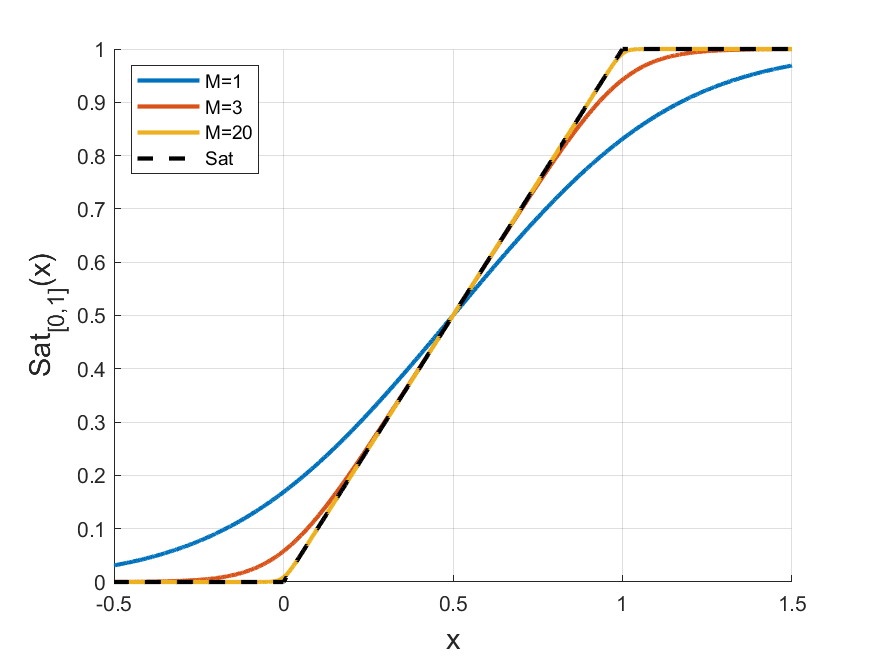
\includegraphics[width=1\textwidth]{Images/SmoothSat}
	\caption{The saturation function and smooth approximation for several values of the tuning parameter.}
	\label{Fig:SmoothSat}
\end{figure}



%\section{UT-Approximated Robust Guidance Problem}
%Let \xut = 
%\begin{align}
%	&\min J = -\bar{h}(v_f) + w_h\sigma_h(v_f) + w_s\sigma_s(v_f) \nonumber\\
%	&\quad\quad\qquad\mathrm{subject\, to }\nonumber \\
%	&\dot{\xl}(v,\param) = \dynamics_v(v, \xl(v,\param), u(v), \param),\quad
%	\xl(v_0,\param) = \state_0(\param) \nonumber\\
%	&\param\sim \normal(\mathbf{0},\cov_{\param}) \nonumber\\
%	&0 \le \ur(v) \le 1 \quad \forall\,v\in [v_0, v_f] \nonumber
%\end{align}

%\section{Necessary Conditions}
%In this section the necessary conditions for an optimal solution to the robust optimal guidance problem are given. Since the terminal objective function has been reformulated as a Lagrange (or running) cost
%\begin{align}
%	J = \int_{v_0}^{v_f}\left[ -\E{h'} +  \frac{w_h}{\sigma_h}(\E{hh'}-\E{h}\E{h'}) + \frac{w_s}{\sigma_s}(\E{ss'}-\E{s}\E{s'})\right]\, \mathrm{d}v
%\end{align}
%and thus the Lagrange cost is
%\begin{align}
%	L(x,u) =  -\E{h'} +  \frac{w_h}{\sigma_h}(\E{hh'}-\E{h}\E{h'}) + \frac{w_s}{\sigma_s}(\E{ss'}-\E{s}\E{s'})
%\end{align}
%The UT approximation of $L$ is given by
%\begin{align}
%	L_{UT}(x,u) =  -\EUT{h'} +  \frac{w_h}{\sigma_h}(\EUT{hh'}-\EUT{h}\EUT{h'}) + \frac{w_s}{\sigma_s}(\EUT{ss'}-\EUT{s}\EUT{s'})
%\end{align}
%
%The Hamiltonian for the UT-approximated ROCP is 
%$H = \lambda^Tf(v,\state(v),\param)+ L(\state,\param)$ 


%%% Local Variables: ***
%%% mode: latex ***
%%% TeX-master: "thesis.tex" ***
%%% End: ***

\chapter{Guidance Assessment Conditions}\label{Ch:AssessmentConditions}

%Also talk about algorithm parameters used to generate trajectories
\section{Entry Conditions and Targets}
The entry guidance strategy is assessed for an MSL-class vehicle with mass $m = 2804$ kg, and area $S = 15.8\, \mathrm{m}^2$. The entry state and associated standard deviations at the entry interface are given in Table~\ref{Table:StateEntryInterface}. By assumption, altitude determines the entry interface point, and thus $\sigma_h = 0$. Given the mean and standard deviation of the entry interface state, a specified prebank angle, and a chosen $v_0$ at which phase 2 guidance begins, the mean and covariance of the state at $v_0$ are determined by integrating Eq.~\eqref{Eq:dynamics:altitude:time}-\eqref{Eq:dynamics:fpa:time} until $v<v_0$. We assume that the distribution remains approximately normal. In practice this appears to be true; the limited aerodynamic nonlinearities at high altitudes do not cause significant changes to the distribution. Note that the parametric uncertainties are also included in determining the mean and covariance at $v_0$.

The resulting mean state and deviations at the start of closed-loop guidance are given in Table~\ref{Table:StateRangeControl}. These are the values used in the solution of the optimal control process. Note that we set $s(v_0) = 0$ for simplicity of discussion, but the total range from the entry interface to the target is 223 km + the optimal range of the solution to the ROGP. 
Similar to the altitude at the entry interface, after propagation to a fixed velocity, $\sigma_v = 0$. The 3$\sigma$ uncertainty in the ballistic coefficient and lift-to-drag ratio is $15\%$. Atmospheric density uncertainty is modeled with the symmetrized Mars Climate Database profile in Fig.~\ref{Fig:DensityVariations}, with the boundary interpreted as the 3$\sigma$ value.
%TODO: Double check these tables, esp EI state. Compare to Guangfei, maybe est with UT in time domain?
\begin{table}[h!]
	\centering
	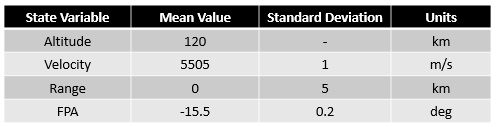
\includegraphics[width=0.85\textwidth]{Images/EntryInterfaceState}
	\caption{The mean state and standard deviations at the entry interface.}
	\label{Table:StateEntryInterface}
\end{table}
\begin{table}[h!]
	\centering
	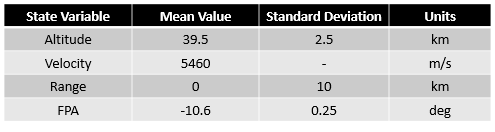
\includegraphics[width=0.85\textwidth]{Images/OptimizationState}
	\caption{The mean state and standard deviations at the start of closed-loop guidance.}
	\label{Table:StateRangeControl}
\end{table}

\section{Robust Optimal Control Solution Parameters}
\begin{table}[h!]
	\centering
	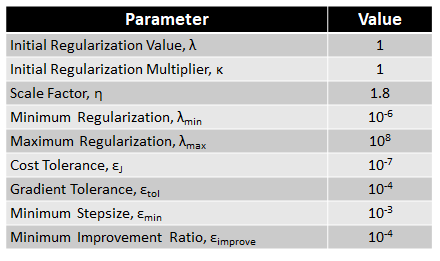
\includegraphics[width=0.75\textwidth]{Images/DDP_Parameters}
	\caption{Algorithm parameters used in all numerical results.}
	\label{Table:DDPParameters}
\end{table}
Table~\ref{Table:DDPParameters} summarizes the algorithm parameters governing the linesearch, regularization, and stopping conditions. 
The smooth saturation approximation uses $M = 20$. The trajectory is discretized into $ N=250 $ velocity steps, with four Euler integration steps per velocity step. The value of $ N $ and the number of integration steps were chosen by validating the terminal altitude and downrange distance against adaptive stepsize integration using MATLAB's \textit{ode45} function. The acceptable error tolerance across all sigma points was 100 m.

\begin{figure}[h!]
	\centering
	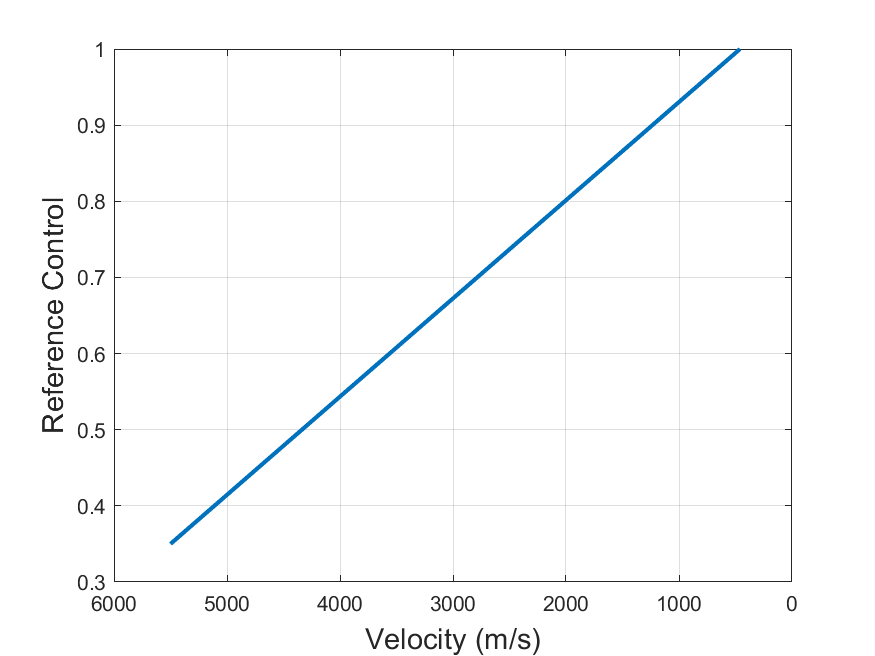
\includegraphics[width=0.75\textwidth]{Images/GuessControl}
	\caption{The reference control used to initialize DDP.}
	\label{Fig:GuessControl}
\end{figure}
%Guess trajectory, show it and discuss. 
A trajectory-control pair is required to initialize the DDP algorithm. In all numerical examples, the initial guess at the optimal reference control is the linear ramp depicted in Fig~\ref{Fig:GuessControl}. This guess is motivated by experience with altitude optimal trajectories, which feature a minimum lift arc followed by a full lift up arc. Such a control has zero margin (in one direction) at every velocity. Our choice is motivated by a similar progression from lift down to lift up, but more gradual and with significant margin throughout. We remark that the solutions are not sensitive to the initial guess. A numerical demonstration is given in Section~\ref{Sec:ConvergenceProperties}.

All solutions consider static gains. In the first section we consider two sets of gains, $K_1=[0,0,0]$ and $K_2 = [0.13,-0.04,-2.5]$, to highlight the impact of the reference trajectory. Later results use jointly optimized gains. For these cases, the initial guess at the optimal gains is the $K_2$. In all examples, unless otherwise noted, the DDP algorithm is applied with the simplification proposed in Subsection~\ref{Sec:DDP_Simplification}.

\subsection{Selecting the UT Parameter}
%Show results for a fixed profile sweeping alpha and show that the estimates are monotonic wrt to the parameter. As result, there exists an alpha that minimizes the error in altitude and range, generally not the same alpha. 

Our earlier example in Section~\ref{Subsec:UQExample} showed that proper selection of $\alpha$ is important, especially for the range variable. In the numerical assessments presented in the Chapter~\ref{Ch:NumericalAssessment}, we consider weight combinations on the grid $w_h\times w_s = [0,3]\times[0,3]$. As such, we selected $\alpha$ to minimize the UT-estimation error in $\sigma_s$ for the optimal solution with $w_h=w_s=1.5$, i.e., at the center point of the grid. We considered integer values of $\alpha$ between 6 and 20, and solved the ROGP for each value. A Monte Carlo simulation was performed for each $\alpha$ and the optimal choice was $\alpha=15$. 
%Note that it is a coincidence that the $\alpha$ in the example of Subsection~\ref{Subsec:UQExample} was the same value. 
% Thinking along the lines, that, minimizing error at the center might keep the error low (enough) at the other points.

\section{Simulation}
%Primary metrics include the 3$\sigma$ low altitude and the 3$\sigma$ range error at the terminal velocity. Some discussion of the mean altitude and range as well. 
Unless otherwise noted, each Monte Carlo simulation is conducted with 3000 sample trajectories. The samples are drawn using Latin Hypercube sampling. The equations of motion are simulated in the time domain, and the bank angle command is updated at a rate of 1 Hz. The bank angle magnitude is subject to the same limits applied during optimization, $0^{\circ}\le|\sigma|\le90^{\circ}$, and the magnitude of the bank angle rate is limited to $20^{\circ}/s$. No bank angle acceleration limit is applied. Range error is the distance between the terminal downrange distance defined by the reference trajectory and the downrange distance flown. The primary metrics we will examine are the 3$\sigma$-low altitude $=\bar{h}-3\sigma_h$ and 3$\sigma$ range error $= 3\sigma_s$ at the final velocity, $v_f=460$m/s. The terminal state distributions are generally non-Gaussian, and in practice percentiles are often used to specify mission requirements. However, metrics based on the mean and standard deviation are presented, because these are the values estimated by the unscented transform, which allows for a direct comparison with the Monte Carlo results.

%WHile simplifcation of models, like the atm density model, introduce conservatism. We simulate using the same models to allow a direct comparison. 

%%% Local Variables: ***
%%% mode: latex ***
%%% TeX-master: "thesis.tex" ***
%%% End: ***

\chapter{Guidance Assessment}\label{Ch:NumericalAssessment}
The proposed guidance law and design method are tested under a variety of circumstances. 

\section{Reference Trajectory Optimization}
In this section we solve the ROGP for a variety of objective weights $(w_h,\,w_s)$ while holding the gains constant. This demonstrates the extent to which the reference trajectory can impact the solution for a fixed set of gains. In the first subsection, we consider the open-loop ($K=K_1=\zero$) scenario to gauge the level of dispersions that must be mitigated by the entry guidance, and the extent to which open-loop covariance shaping can impact performance. MSL entry guidance designers performed a similar exercise~\cite{MSL_EDL2}. The second subsection repeats the sweep over the weights in a closed-loop scenario with $K=K_2$.

\subsection{Open-Loop Optimization}
Figure~\ref{Fig:MCResultsOpenLoop} presents contours of the Monte Carlo estimated 3$\sigma$-low altitude and range errors. The 3$\sigma$ range errors vary from 59 to 66 km, while the 3$\sigma$-low altitude varies from 7.8 km to 10.6 km. Increasing the weight $w_s$ reduces range errors as intended, but comes at a penalty to altitude performance. The results also highlight the large magnitude of the terminal state variations arising from the variations in the initial state and model uncertainty, and the limited extent to which the reference trajectory can alter the terminal statistics without feedback.
%TODO: Show some control profiles? 
\begin{figure}[h!]
	\centering
	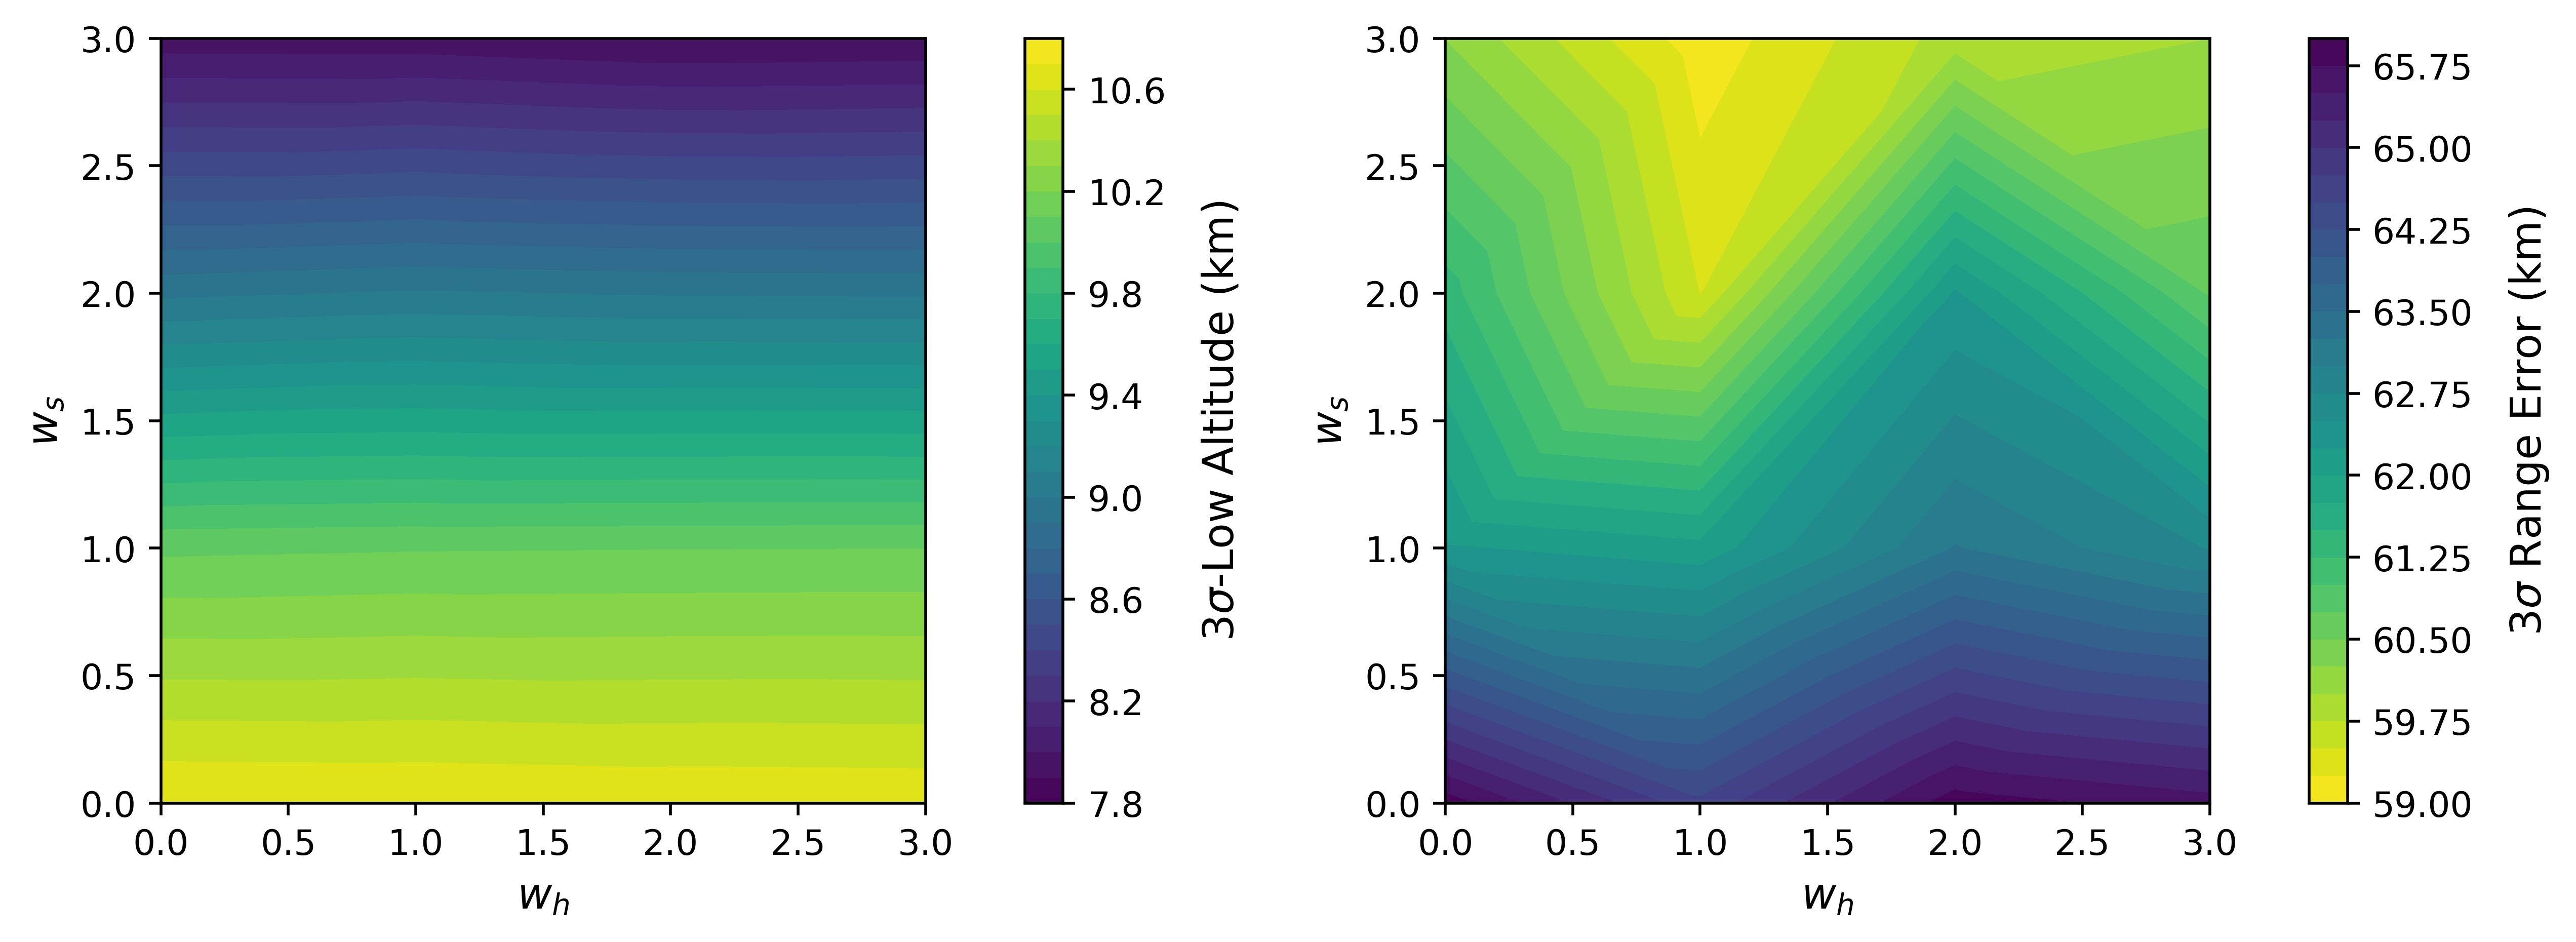
\includegraphics[width=1\textwidth]{Images/OpenLoop_WeightSweepMCResults}
	\caption{Monte Carlo statistics for the open-loop trajectory optimization. }
	\label{Fig:MCResultsOpenLoop}
\end{figure}
%\begin{figure}[h!]
%	\centering
%	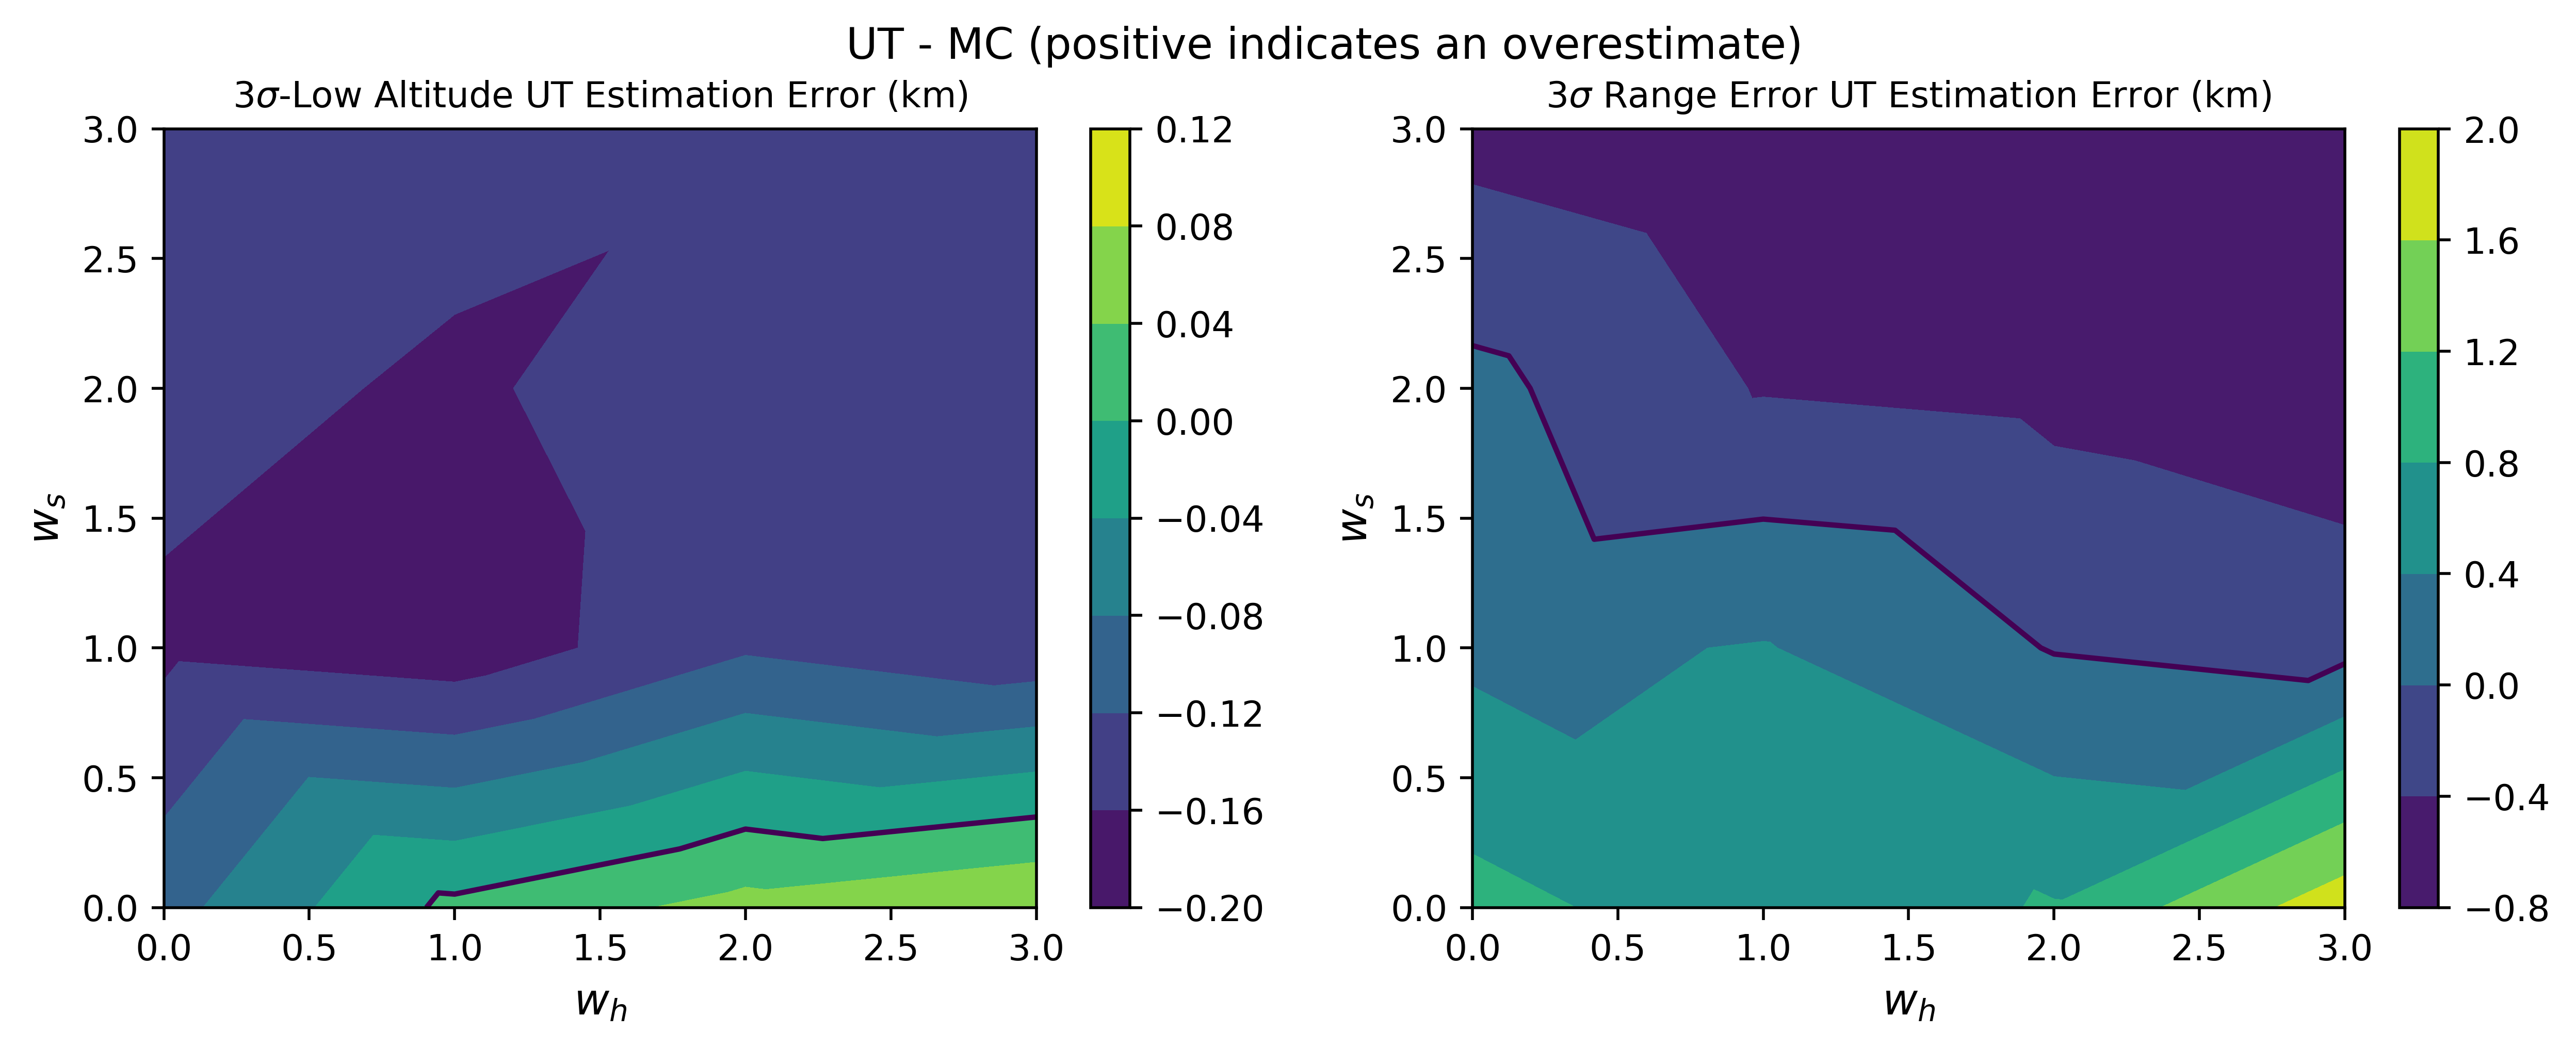
\includegraphics[width=1\textwidth]{Images/Reoptimized_WeightSweepError}
%	\caption{}
%	\label{Fig:MCErrorsOpenLoop}
%\end{figure}

\subsection{Closed-Loop Optimization}
%Maybe show ONLY  Monte Carlo results here. Then in the next section, do a detailed comparison. Justified by the fact that optimized gains are what we would want to use, so we should confirm those? But MC here already confirms. We could maybe get away with showing the UT only
Figure~\ref{Fig:MCResultsFixedGain} presents contours of the Monte Carlo estimated 3$\sigma$-low altitude and range errors for the closed-loop guidance with $K=K_2$. Introducing feedback allows the guidance to achieve 3$\sigma$ range errors as low as 5.6 km while also keeping the 3$\sigma$-low altitude above 9 km. This low altitude can be raised to 9.7 km at the expense of growing the 3$\sigma$ range errors to 14.6 km. The largest range errors occur when optimizing purely for mean altitude, $w_h=w_s=0$. 
\begin{figure}[h!]
	\centering
	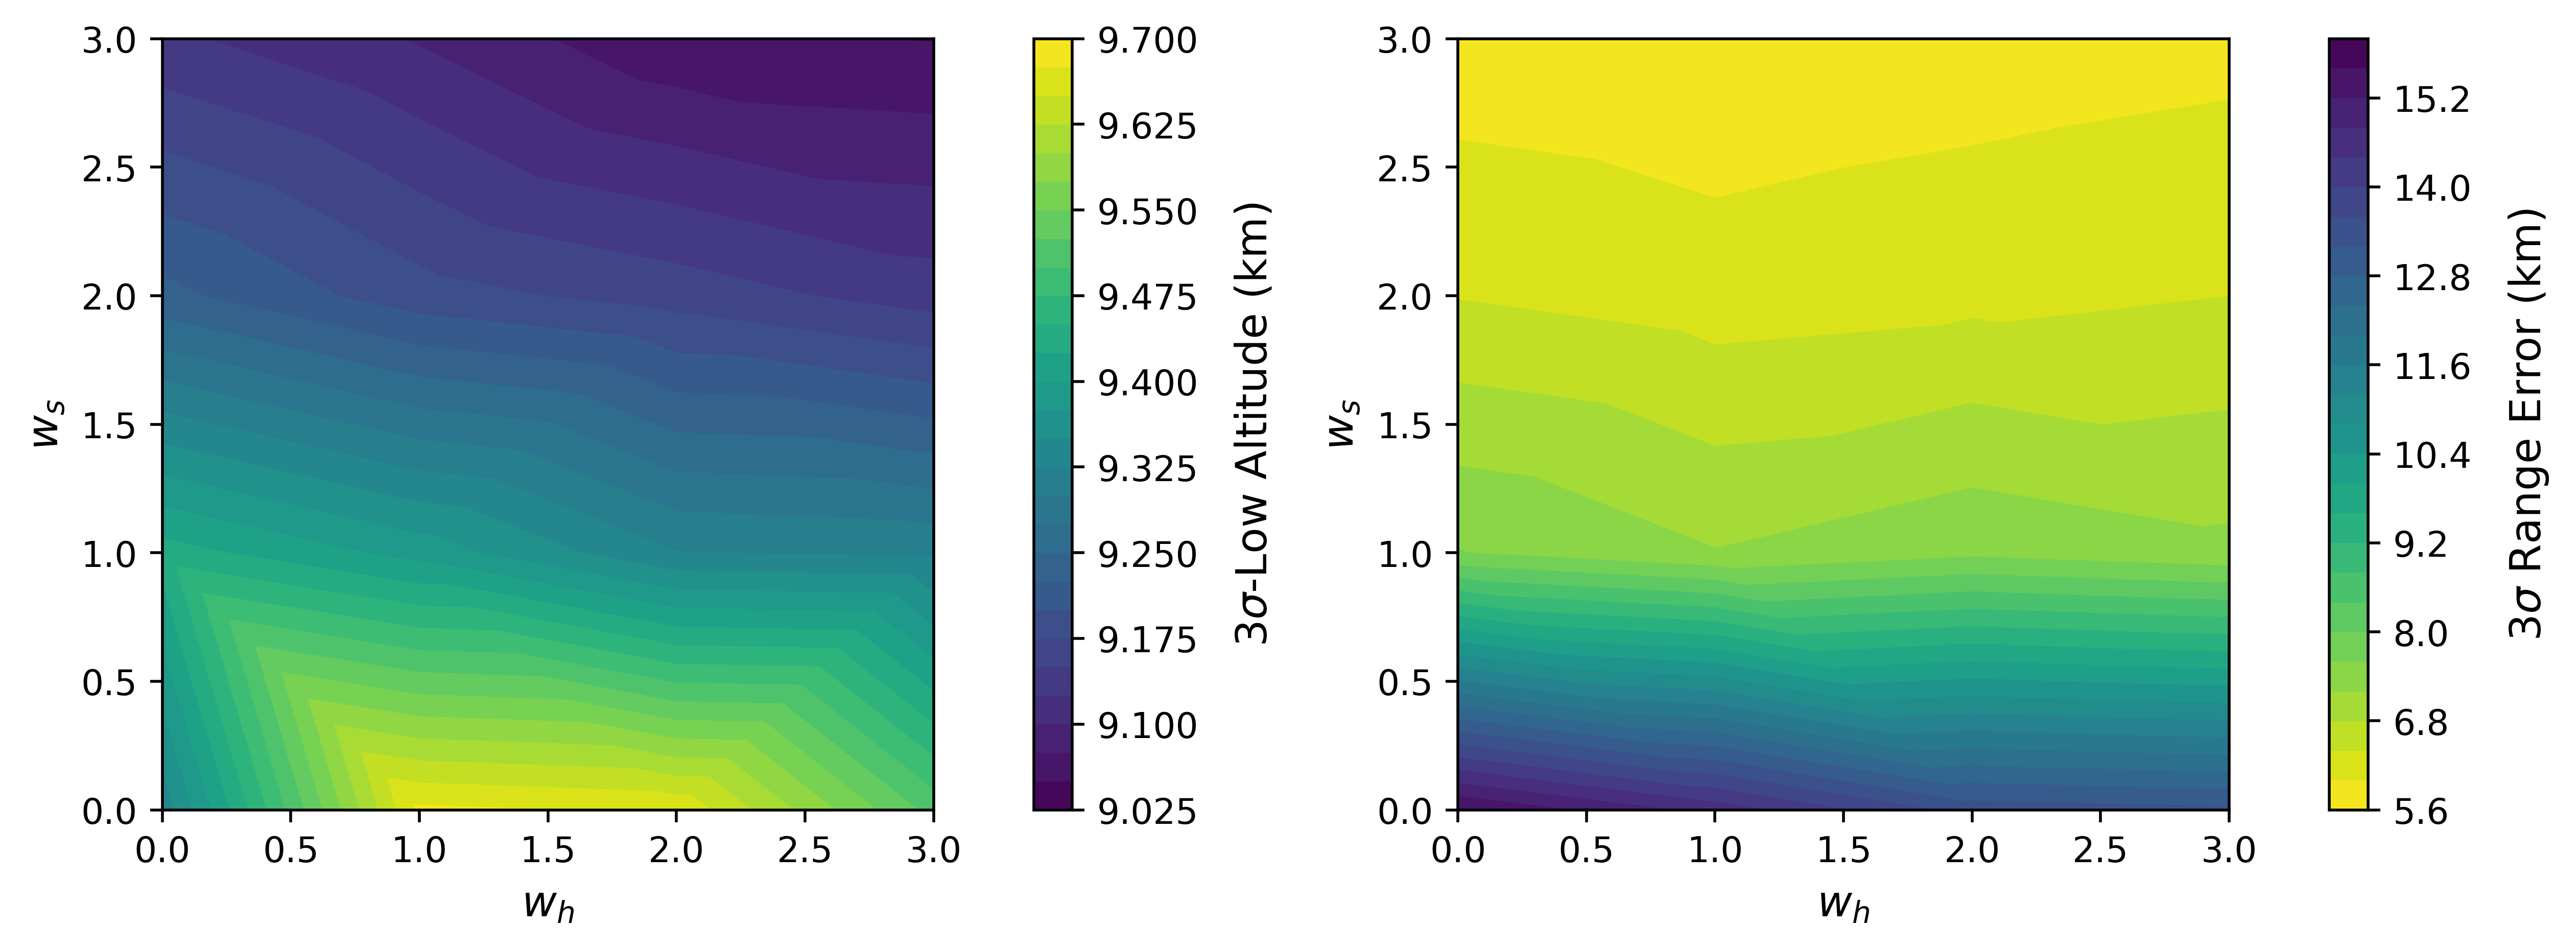
\includegraphics[width=1\textwidth]{Images/Reestimated_WeightSweepMCResults}
	\caption{Monte Carlo statistics for the closed-loop trajectory optimization with static gains.}
	\label{Fig:MCResultsFixedGain}
\end{figure}
Figure~\ref{Fig:MCErrorsFixedGain} shows the contours of the errors in the UT statistics compared to the Monte Carlo results. The error in 3$\sigma$-low altitude varies between a 120 m overestimate and a 360 underestimate. For a majority of $(w_h,w_s)$ pairs, the low altitude is underestimated. Although the estimation errors are generally small, they are large enough to affect the optimality of the solutions. The 3$\sigma$-low altitude should be maximized when $w_h=3$ and $w_s=0$, but instead the highest 3$\sigma$-low altitude is achieved for $w_h=1.5$. Notice that the suboptimality is also small, the solution for $w_h=3$ is only 150 m lower than for $w_h=1.5$. In contrast, the smallest range errors do occur for the $w_h=0,\,w_s=3$. 
\begin{figure}[h!]
	\centering
	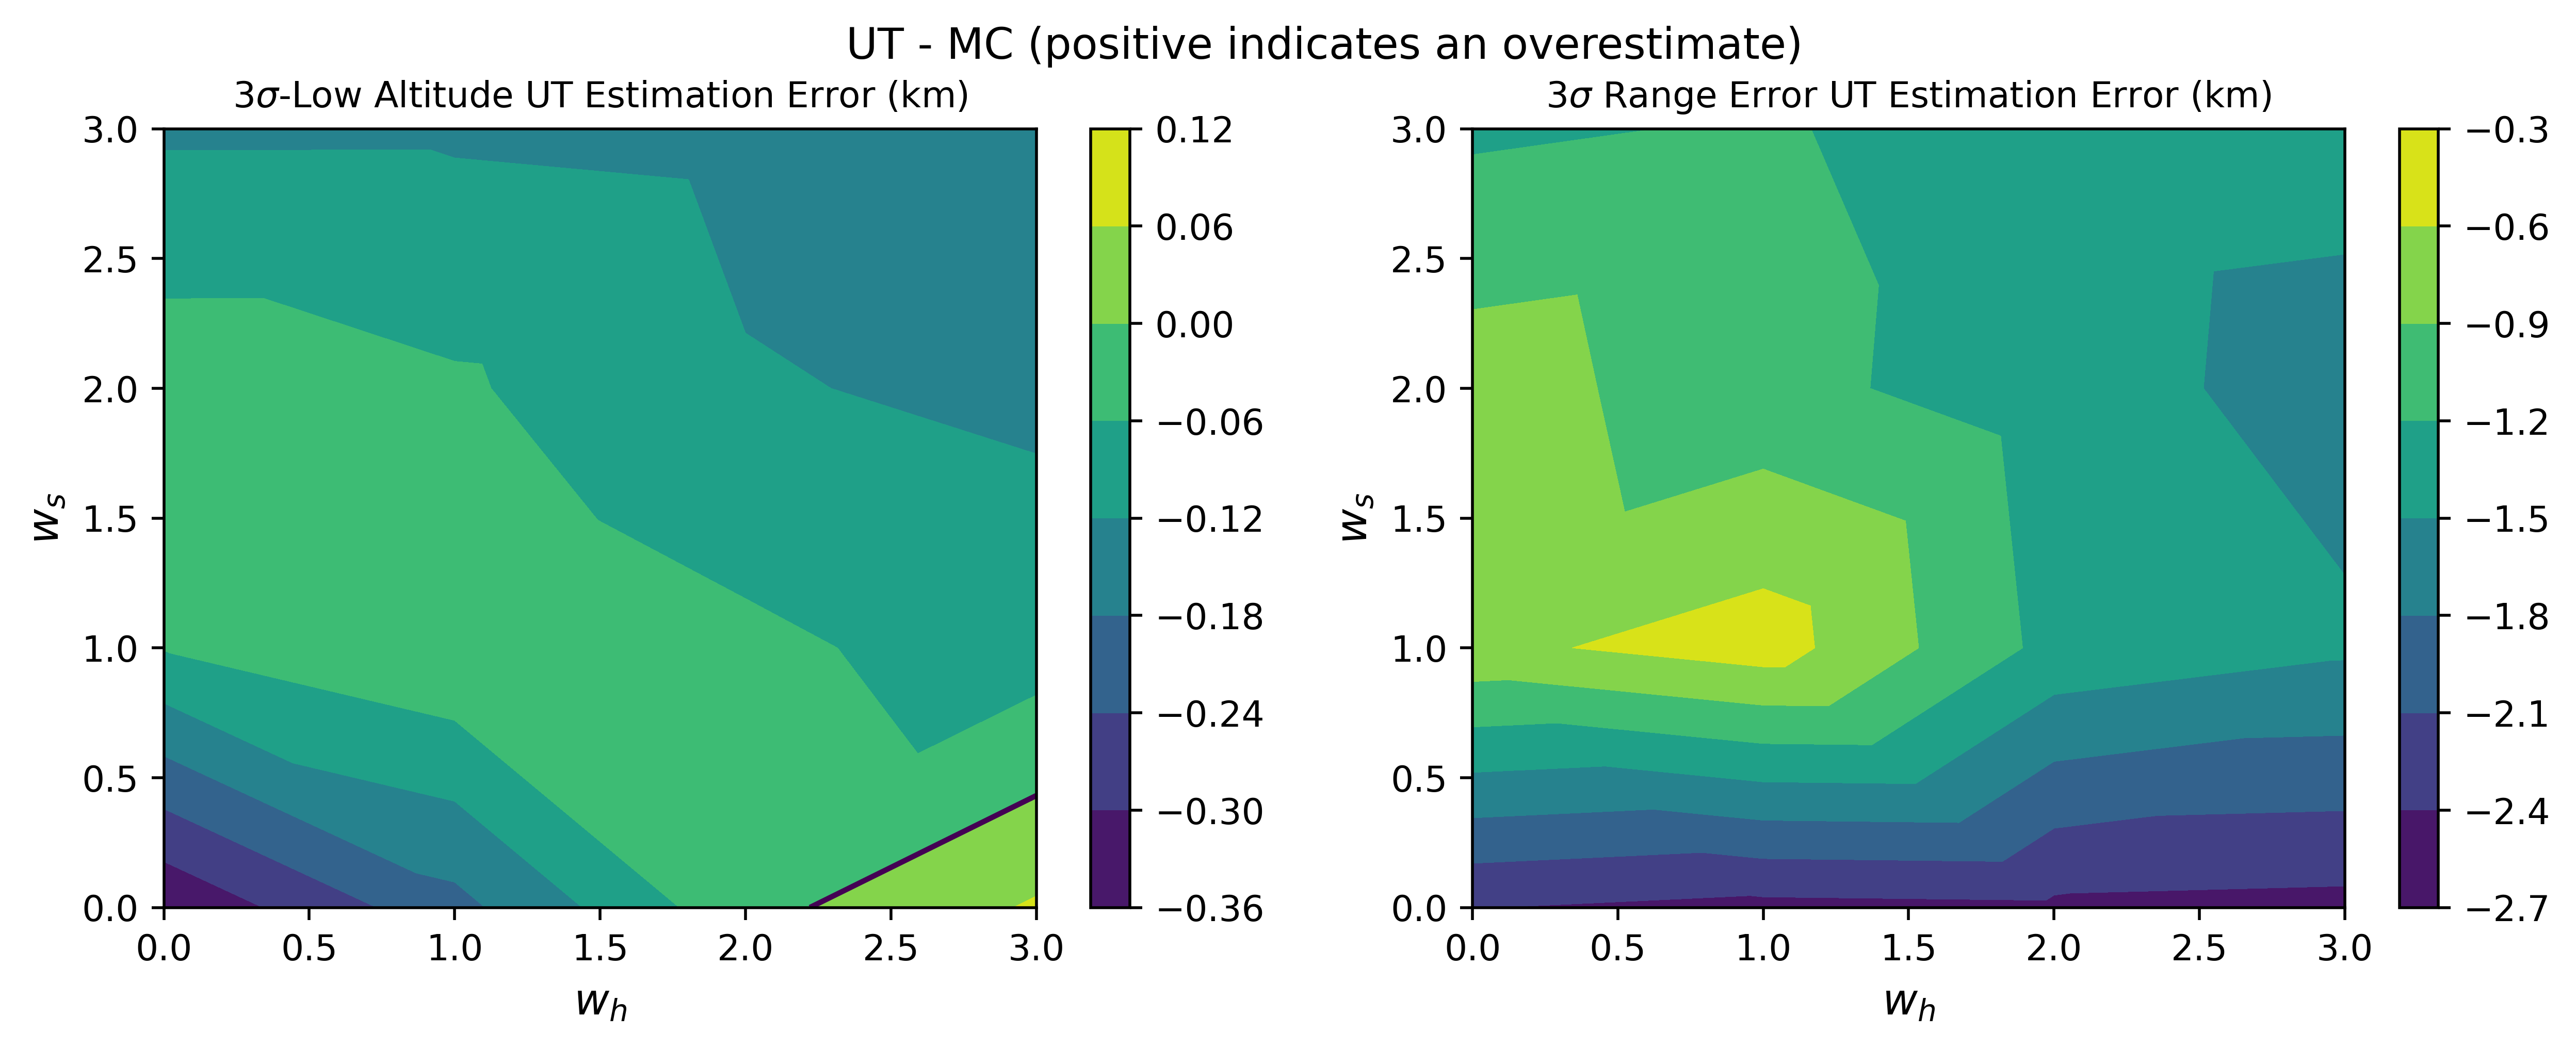
\includegraphics[width=1\textwidth]{Images/Reestimated_WeightSweepError}
	\caption{Unscented Transform estimation errors relative to Monte Carlo statistics for trajectory optimization with static feedback gains.}
	\label{Fig:MCErrorsFixedGain}
\end{figure}

\section{Joint Gain Optimization}
%Motivate the constant gain optimization here by showing an example of bad MC performance when simultaneously optimizing velocity-varying gains? Then show how well the constant gains can do when jointly optimized. 
In this section, the ROGP is again solved for a variety of weights but now the gains are treated as design parameters, and the DDP modification presented in Subsection~\ref{Sec:DesignOptimization} is used to jointly optimize them alongside the reference trajectory and control. As one might intuitively expect, the effect on the range of solutions is much more extreme with joint optimization than without. 

Figure~\ref{Fig:MCResultsOptGain} shows the contours. An additional 800 meters of low altitude can be gained (relative to the previous solutions with unoptimized gains), but at the expense of large $3\sigma$ range errors (above 40 km). However, a very tight range distribution of $3\sigma_s = 3$ km can be achieved while still maintaining a 9 km 3$\sigma$-low altitude for a variety of weights. The range error stops improving at approximately $w_s=1$, but the low altitude continues to decrease as $w_s$ is raised. Thus, an effective compromise might be $w_h=w_s=1$. 
%TODO: A Common trend among Figures~\ref{Fig:MCResultsOpenLoop},\ref{Fig:MCResultsFixedGain}, and \ref{Fig:MCResultsOptGain} is the relatively weak influence of $w_h$. While some weight prevents large altitude losses, even large weights cannot achieve more than a few hundred meters of improvement. 
\begin{figure}[h!]
	\centering
	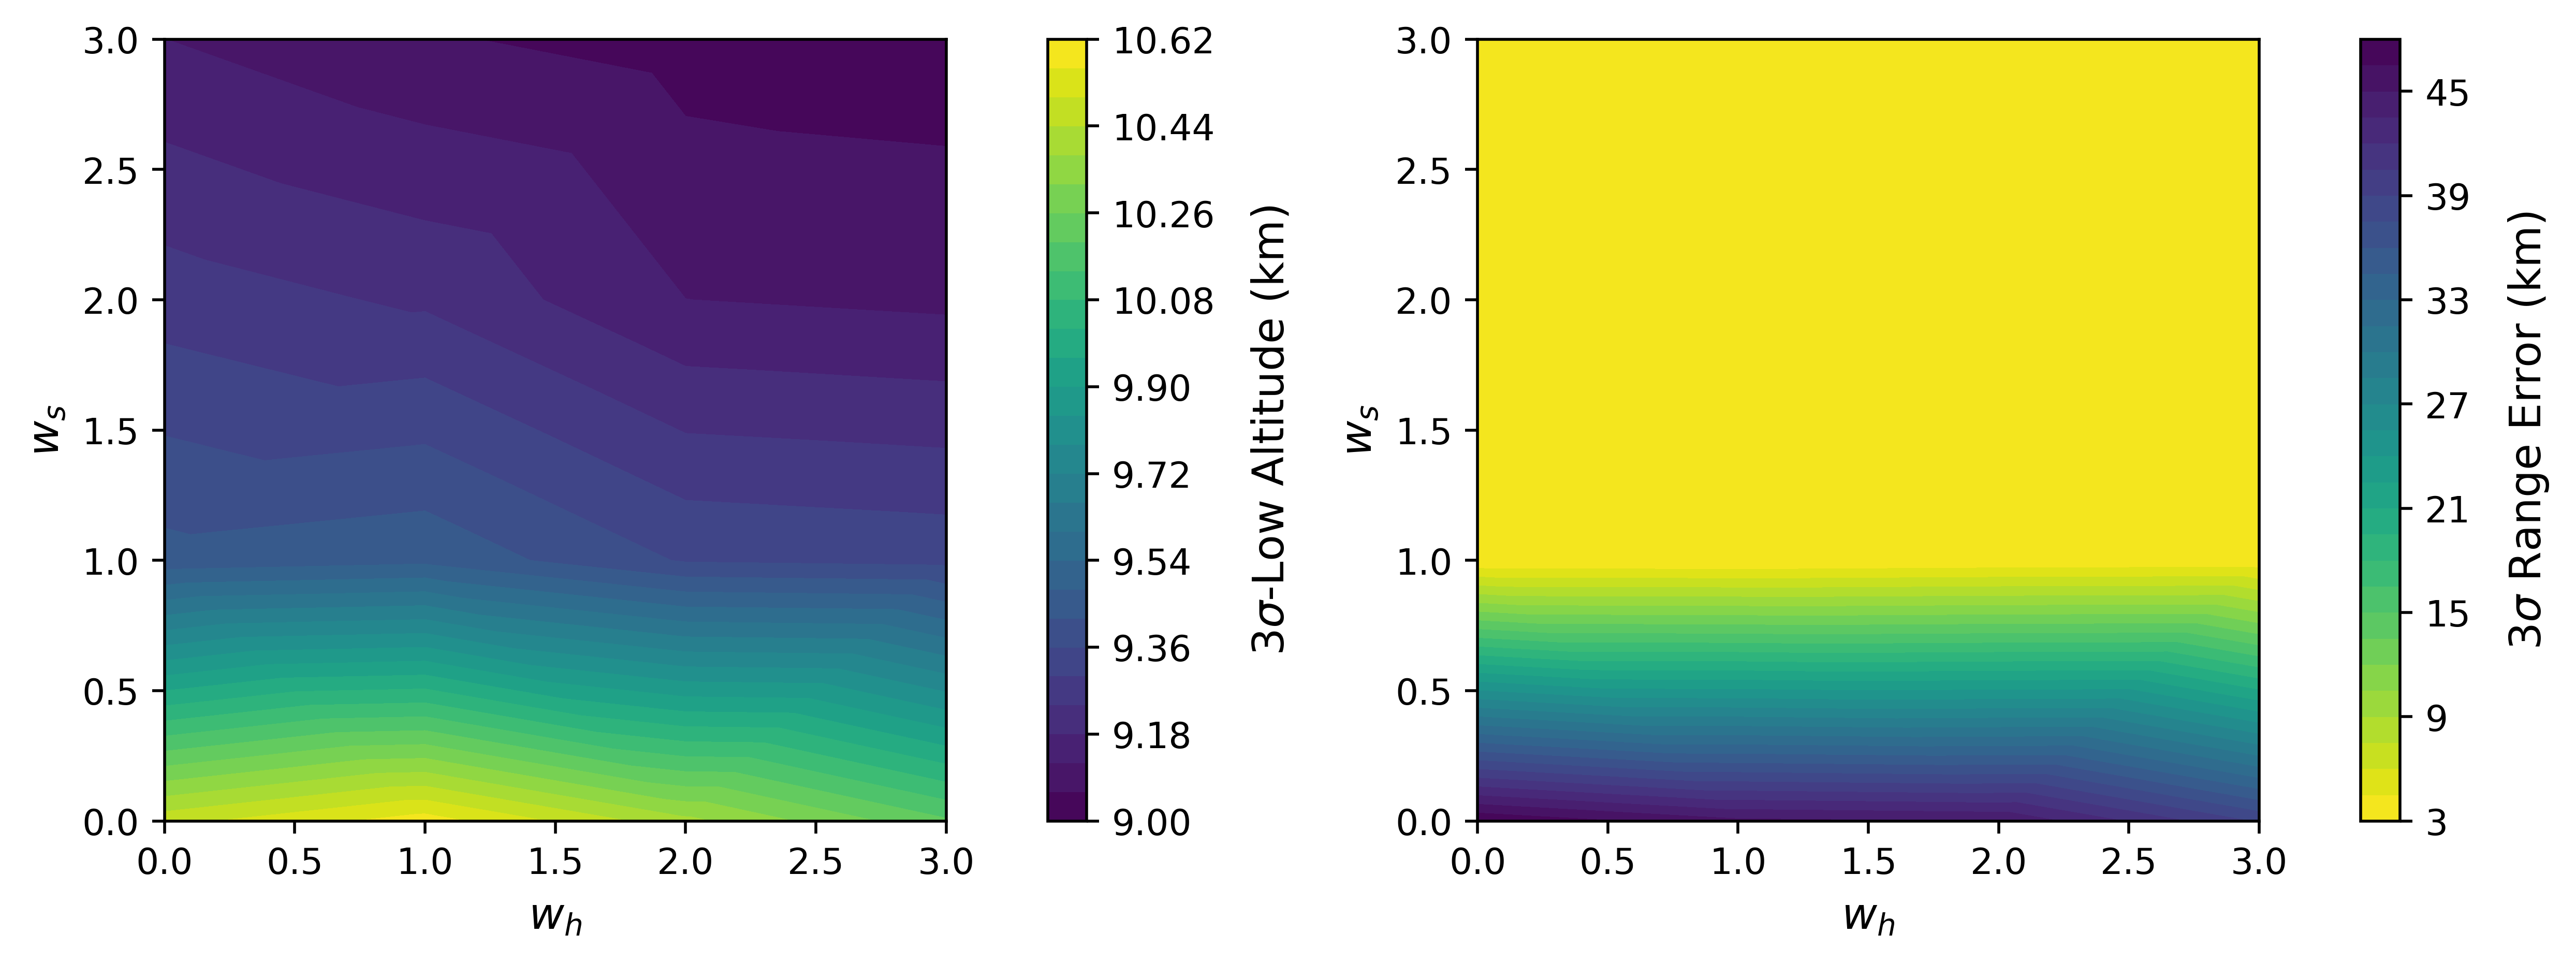
\includegraphics[width=1\textwidth]{Images/Reoptimized_WeightSweepMCResults}
	\caption{Monte Carlo statistics for jointly optimized static feedback gains.}
	\label{Fig:MCResultsOptGain}
\end{figure}
Figure~\ref{Fig:MCErrorsOptGain} shows the contours of the errors in the UT statistics compared to the Monte Carlo results. The dark line in each plot is the zero contour, where the UT and MC agree with approximately no error. Comparing Fig.~\ref{Fig:MCErrorsOptGain} to the previous error contour, Fig.~\ref{Fig:MCErrorsFixedGain}, we can see the effect to selecting the UT scaling parameter to minimize the estimation error in range error. For the fixed gain results in Fig.~\ref{Fig:MCErrorsFixedGain}, the range errors were uniformly underestimated, while for the optimized gains, the zero contour passes through $(w_h,w_s) = (1.5,1.5)$. 
The error in 3$\sigma$-low altitude varies between a 120 m overestimate and a 200 underestimate. Like the fixed gain results, the low altitude is underestimated for a majority of $(w_h,w_s)$ pairs. Estimation errors once again affect the optimality of the solutions. The highest 3$\sigma$-low altitude is achieved for $w_h=1$. 
\begin{figure}[h!]
	\centering
	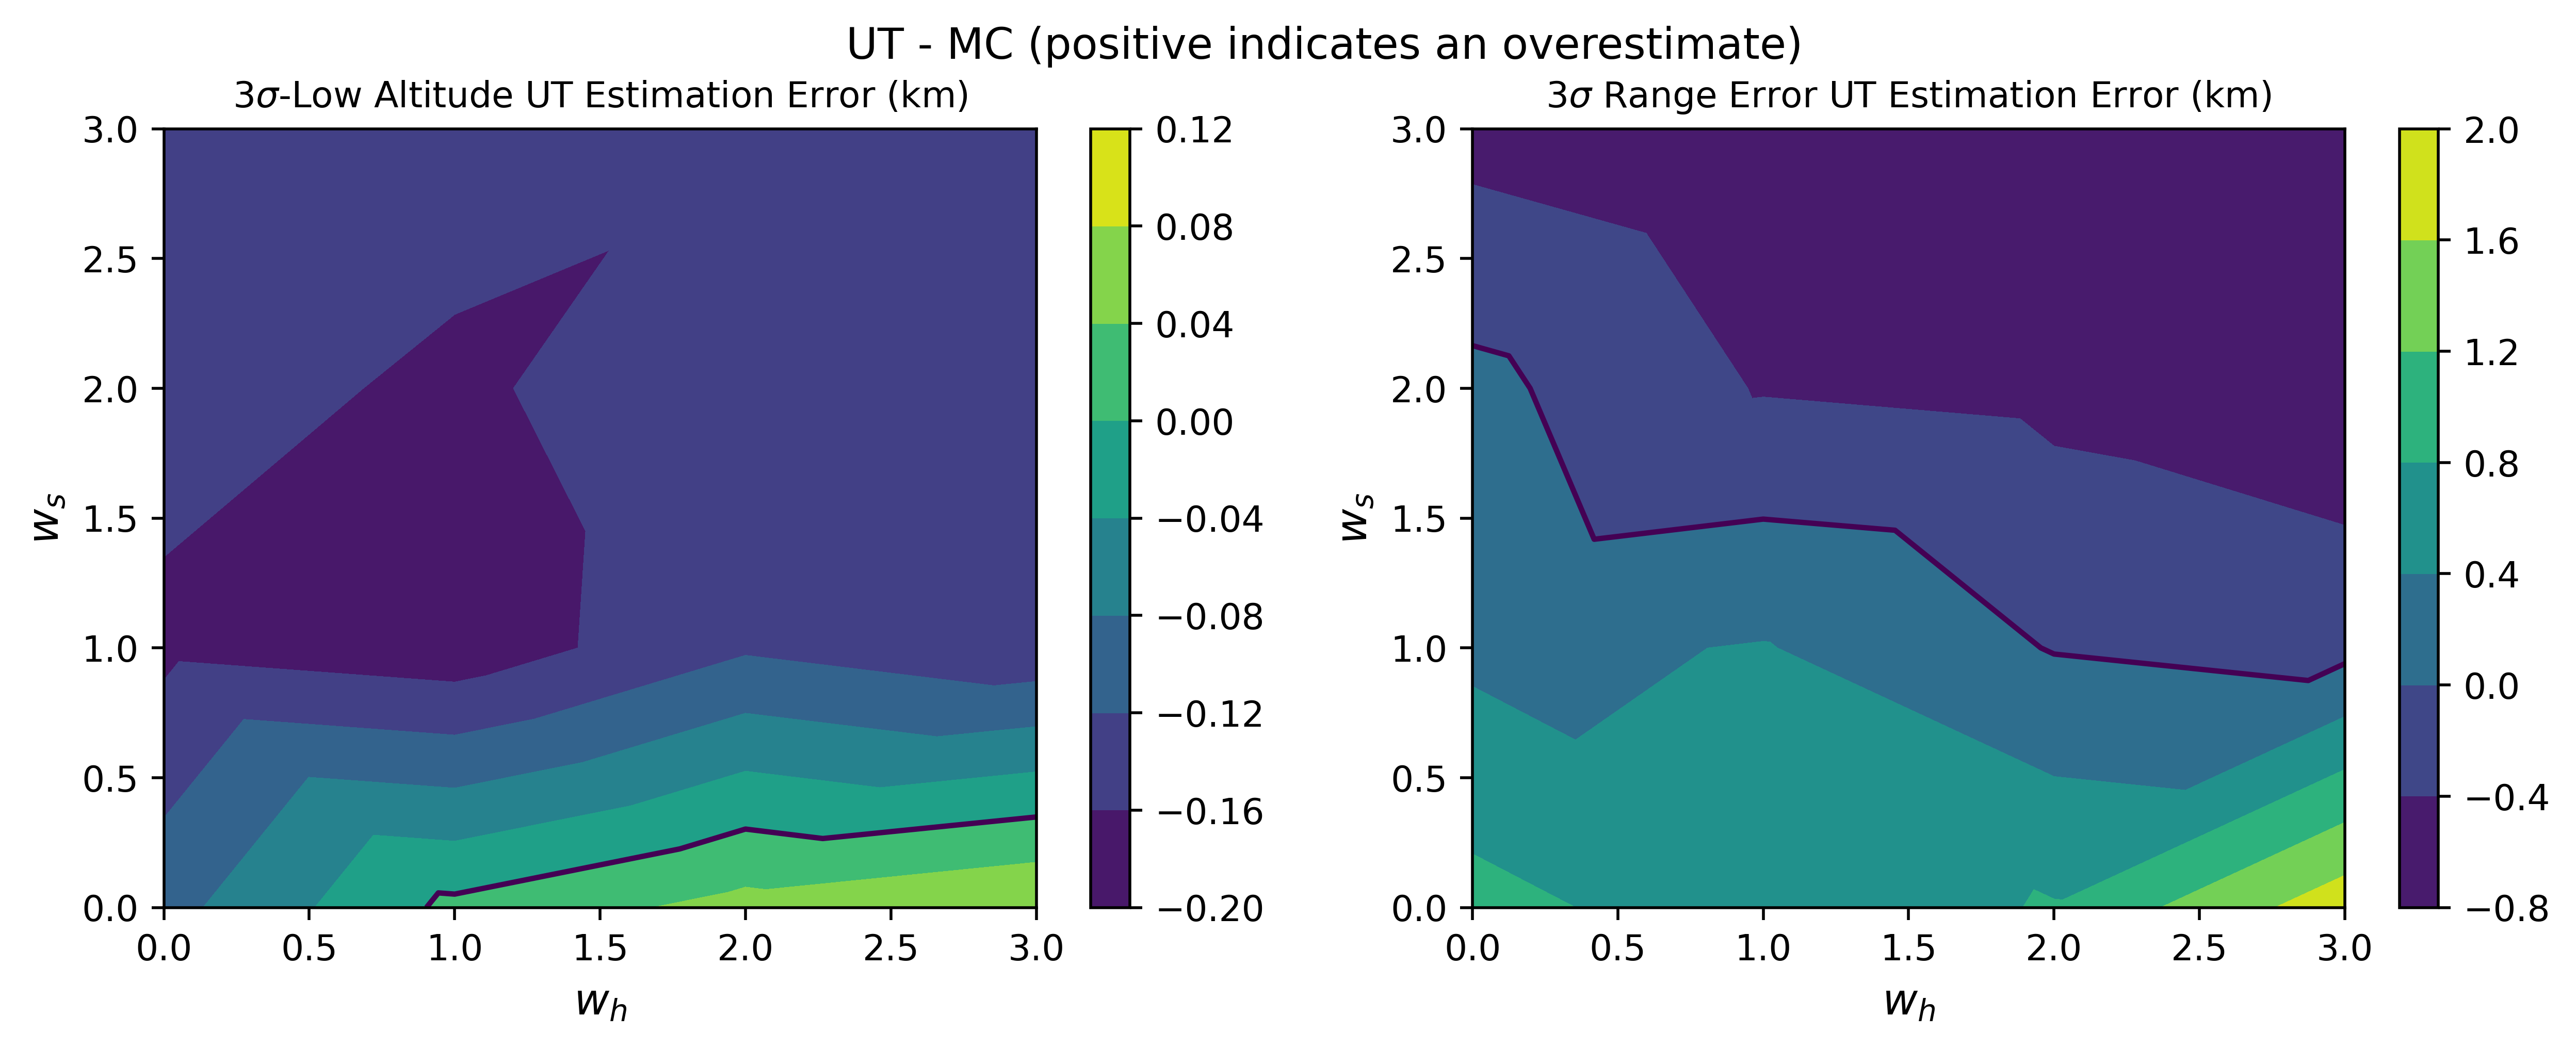
\includegraphics[width=1\textwidth]{Images/Reoptimized_WeightSweepError}
	\caption{Unscented Transform estimation errors relative to Monte Carlo statistics for jointly optimized static feedback gains.}
	\label{Fig:MCErrorsOptGain}
\end{figure}
Figure~\ref{Fig:MCTargetRange} depicts how the optimal downrange distance resulting from the solution to the ROGP varies with the weights. A very clear general trend is that more robust solutions, i.e., those with higher weight on either standard deviation, tend to target longer downrange distances. The total variation in target distance is about 30 km. The feedback gains have a large impact on these results. For comparison, Fig~\ref{Fig:MCTargetRangeOpenLoop} shows the target distances arising from the unguided open-loop optimization (corresponding to the contour in Fig.~\ref{Fig:MCResultsOpenLoop}). In the unguided case, there is virtually no change in target distance for different $w_h$, and the variation is exclusively with respect to $w_s$. The target distances are also noticeably shorter than in the guided case, roughly 40 km shorter on average.  
\begin{figure}[h!]
	\centering
	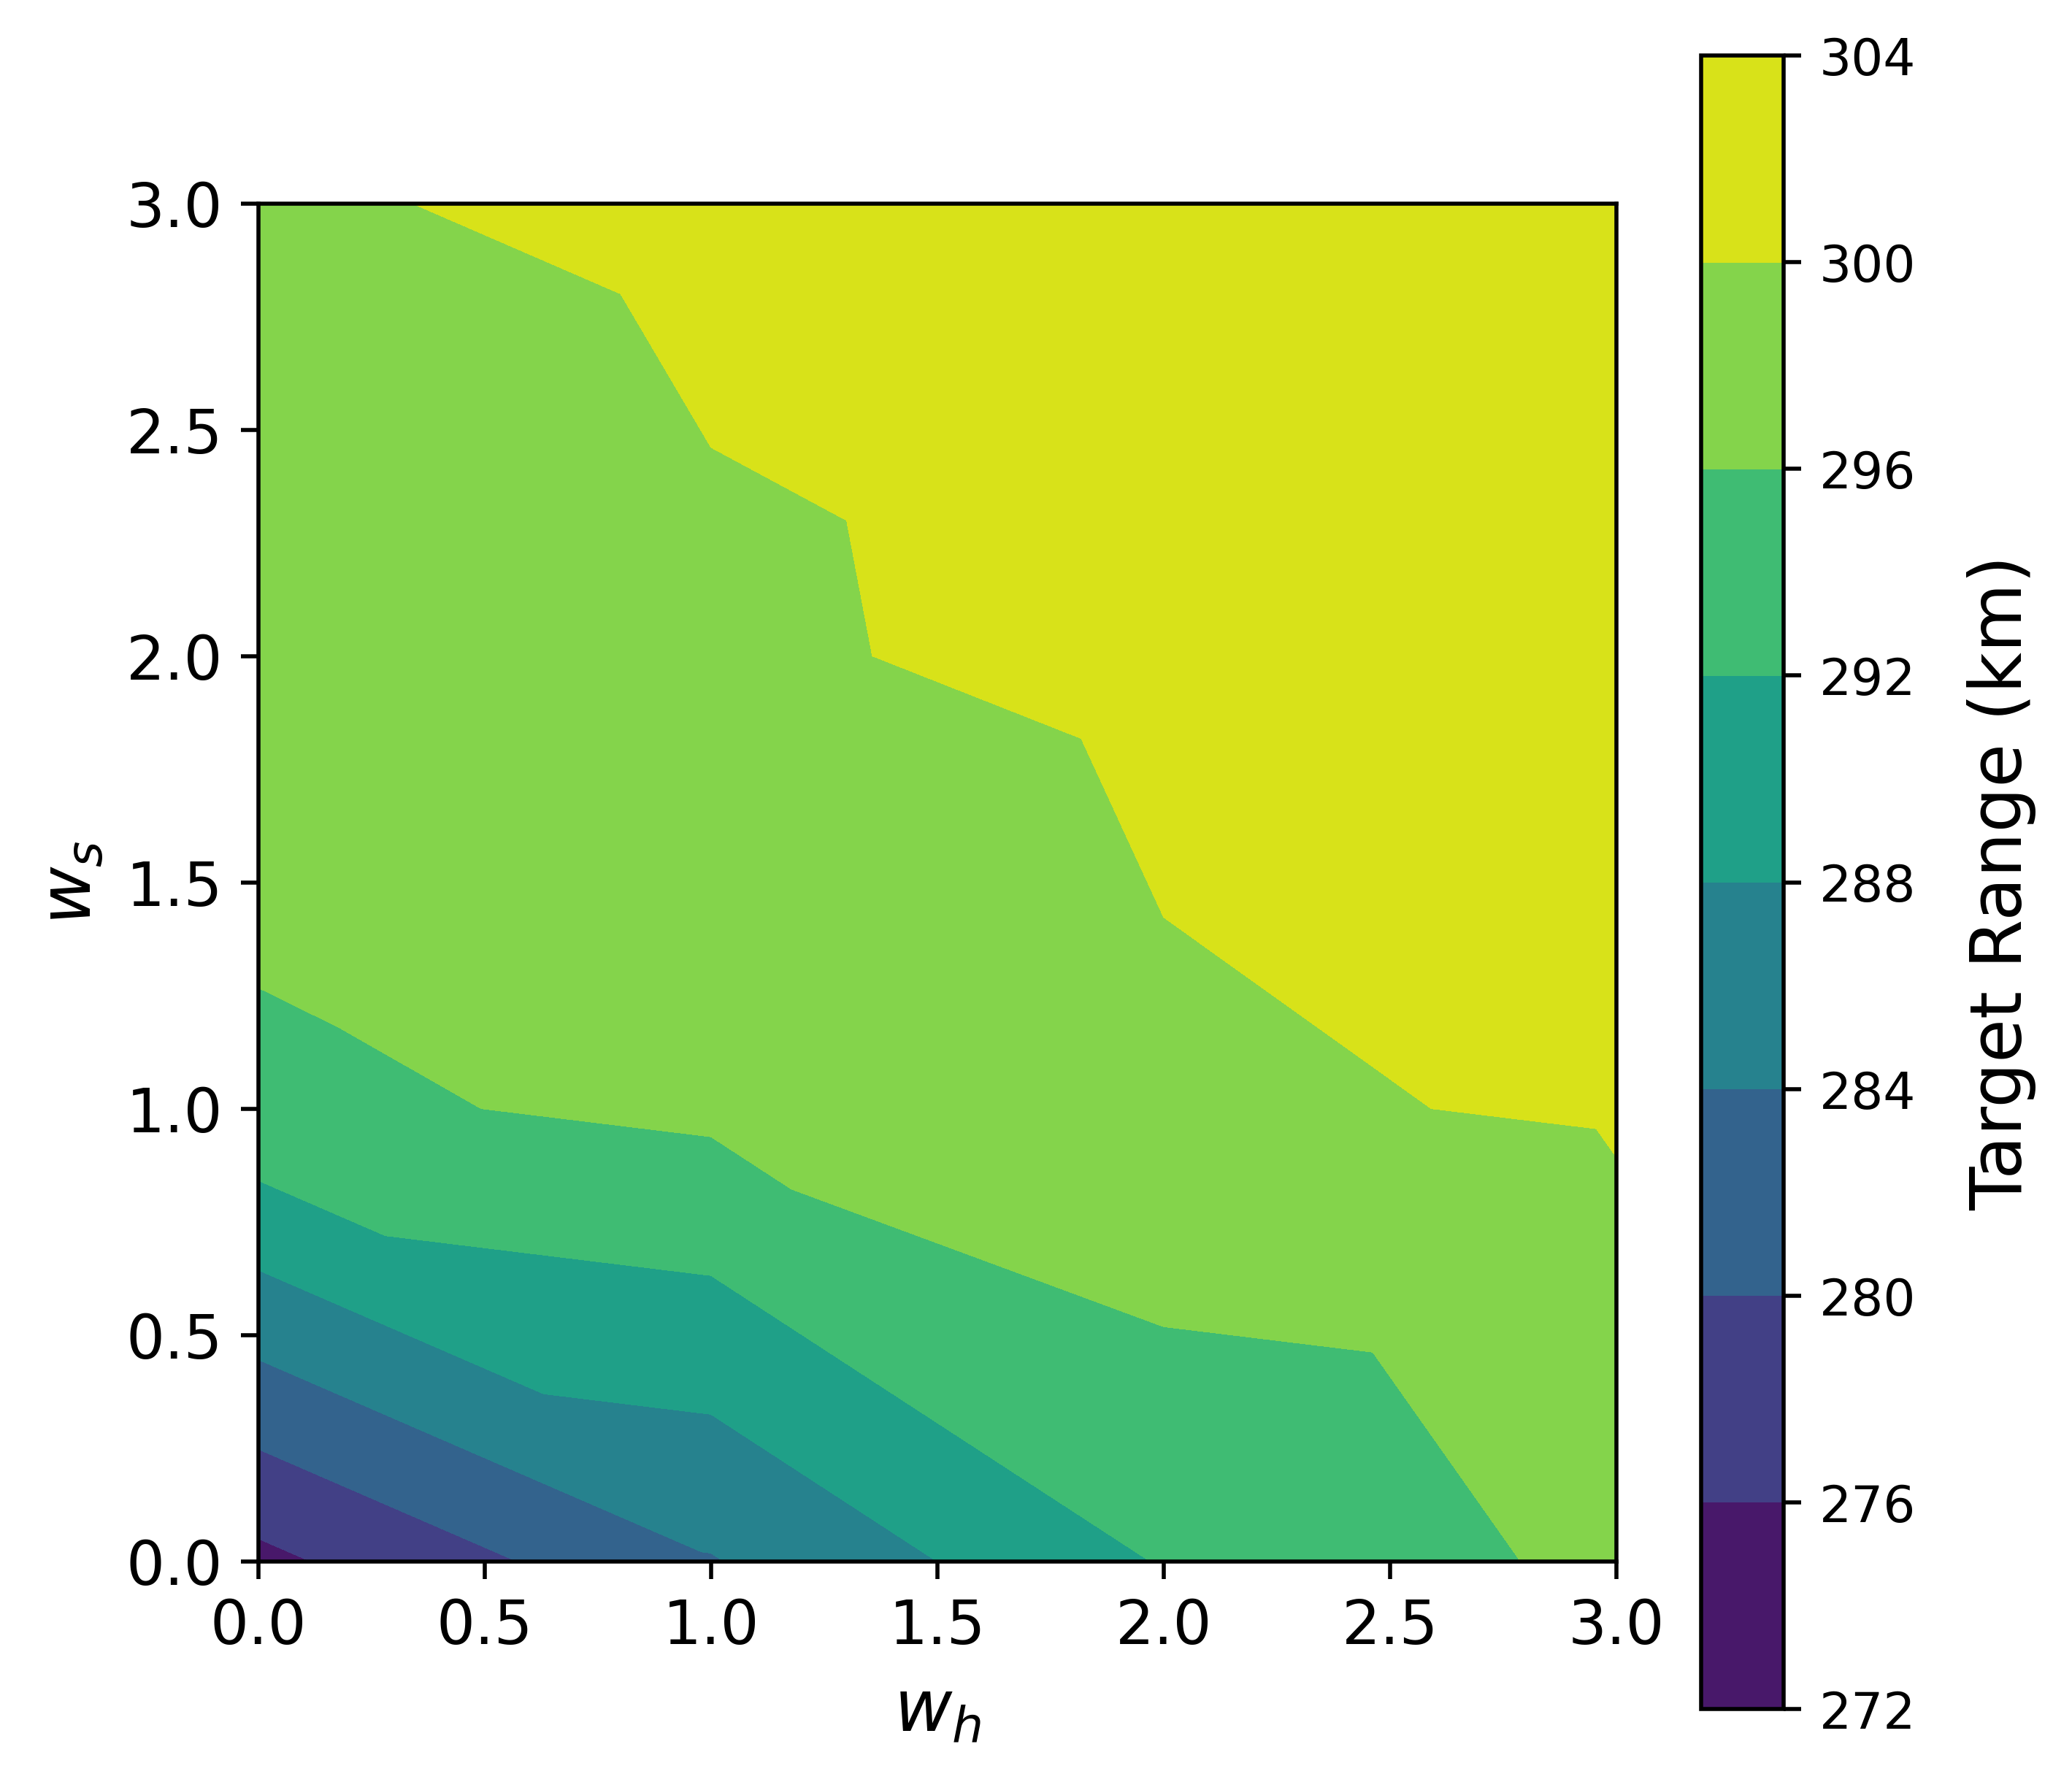
\includegraphics[width=1\textwidth]{Images/MSL_TargetRange}
	\caption{The optimal target range as a function of the performance weights.}
	\label{Fig:MCTargetRange}
\end{figure}
\begin{figure}[h!]
	\centering
	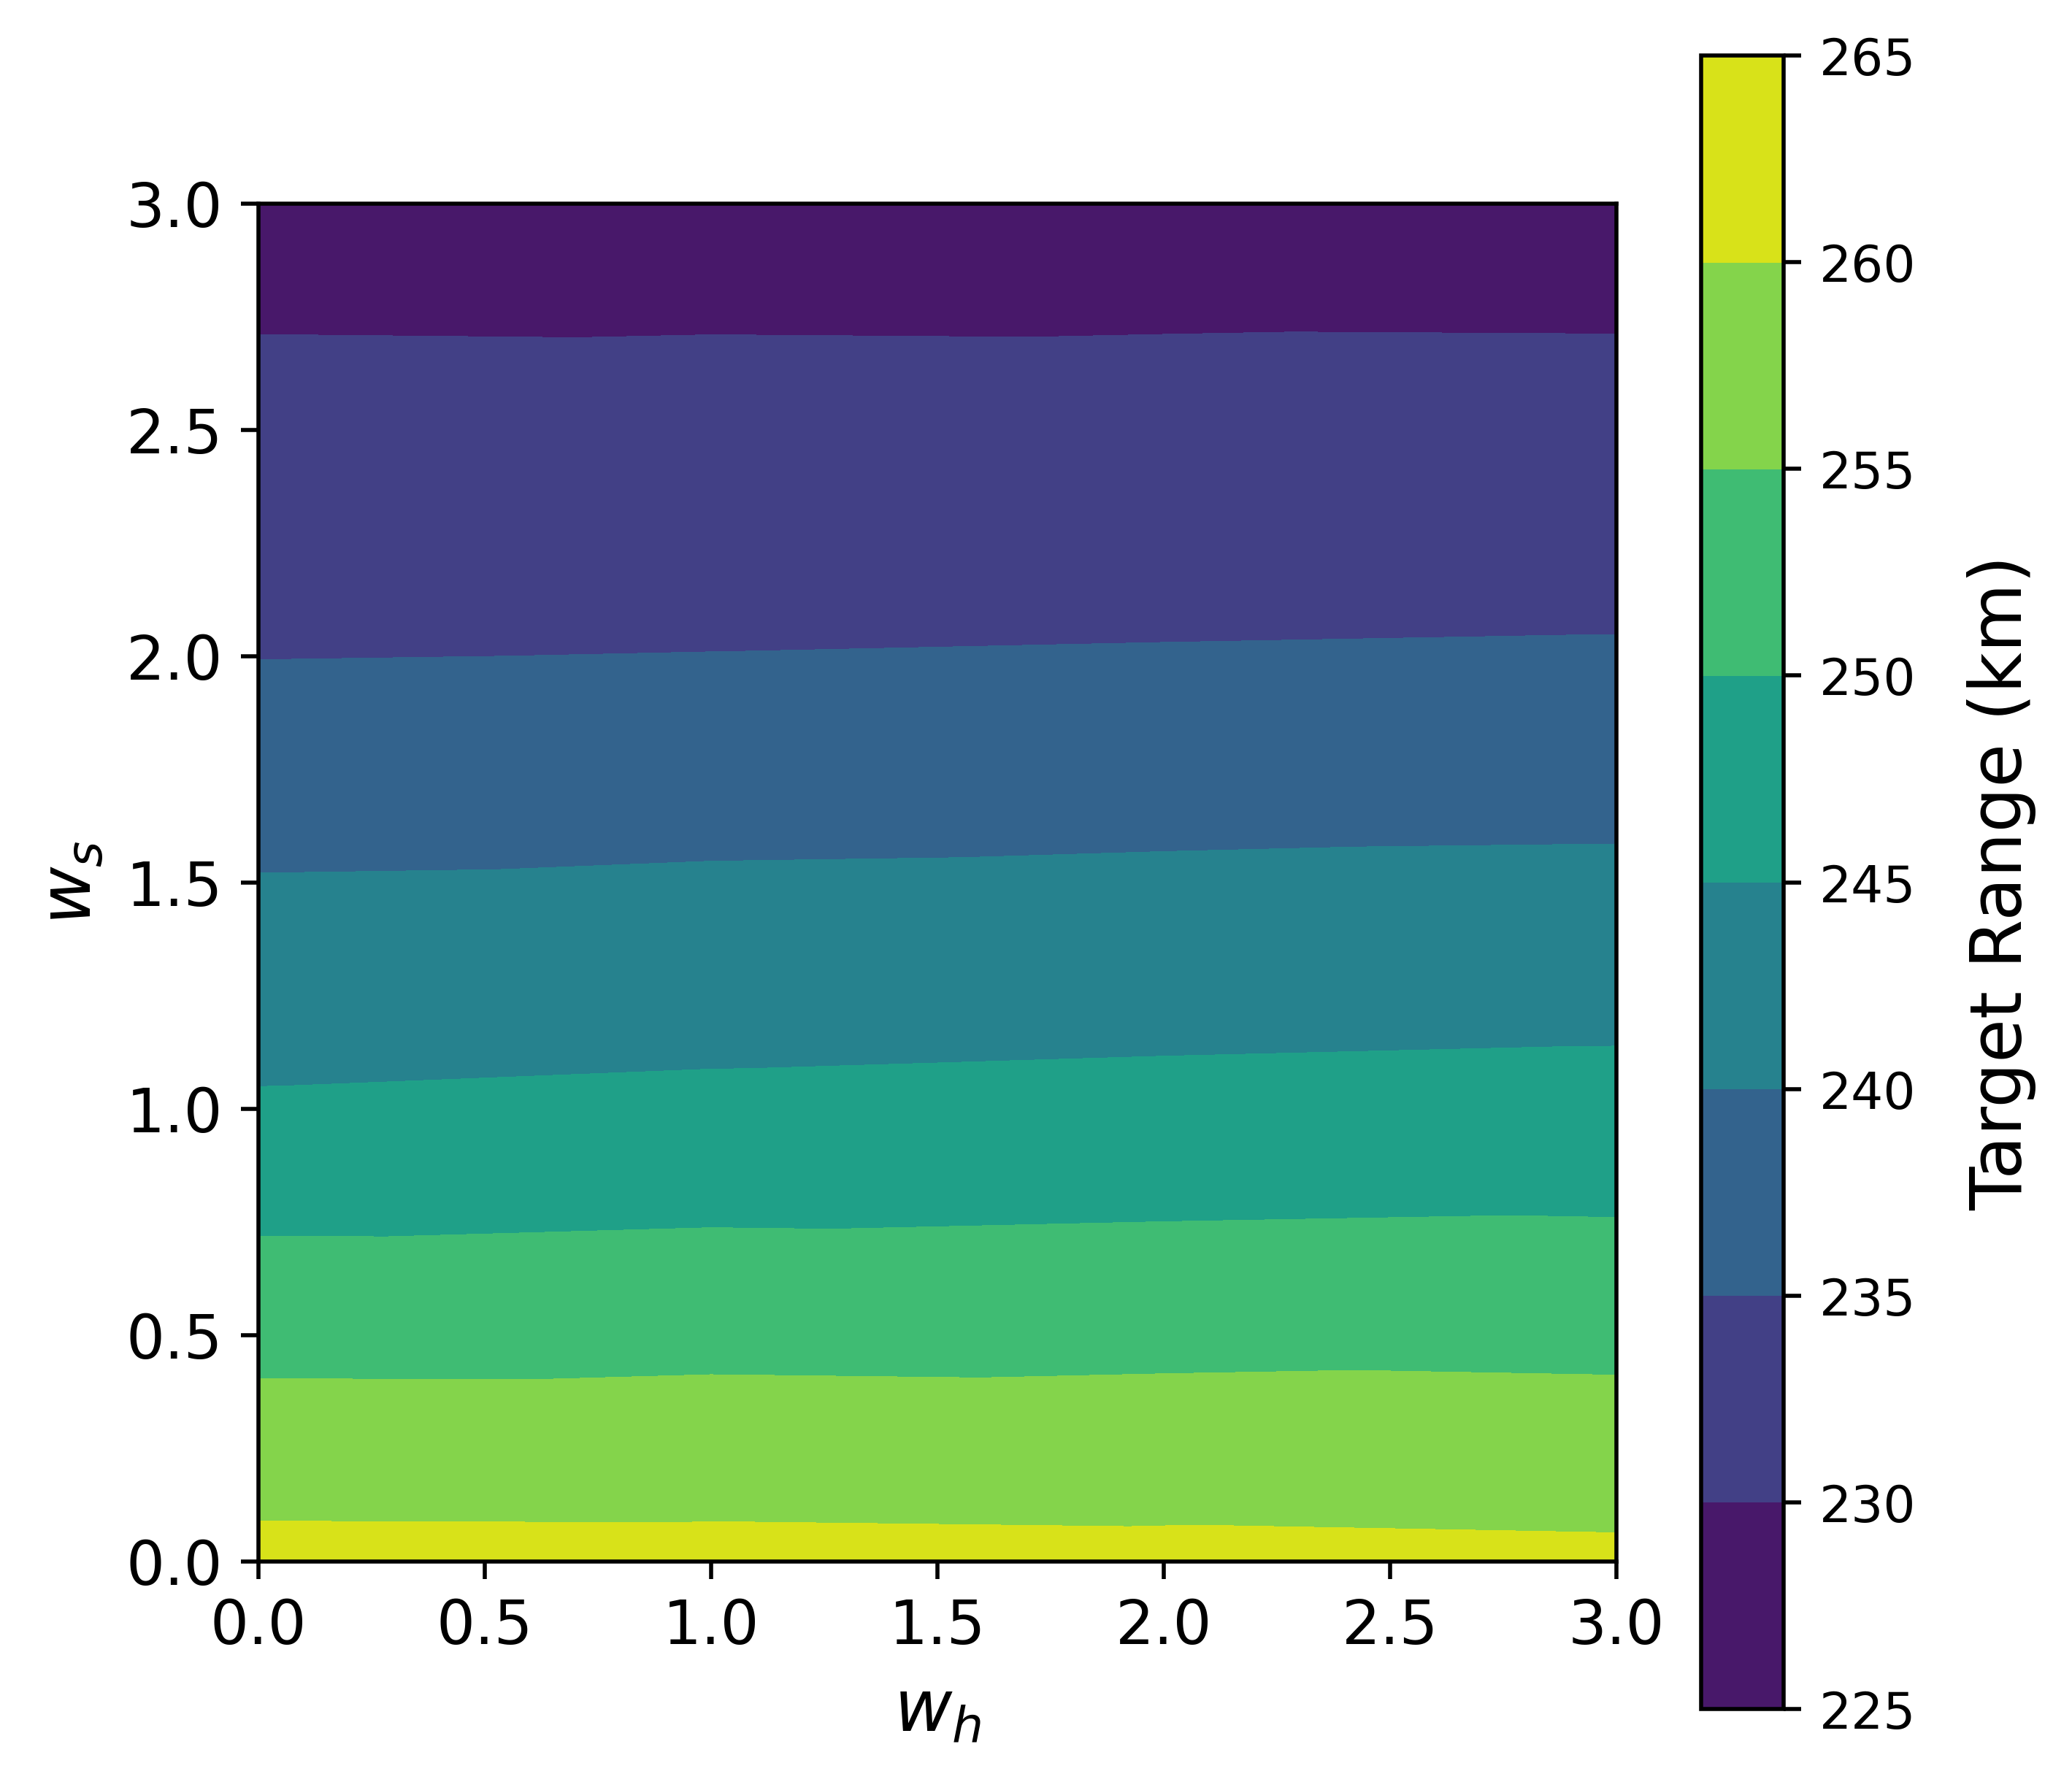
\includegraphics[width=1\textwidth]{Images/OpenLoop_TargetRange}
	\caption{The optimal target range as a function of the performance weights for an unguided vehicle.}
	\label{Fig:MCTargetRangeOpenLoop}
\end{figure}

\section{Detailed Comparison}
Other sections are input-output, examining the tradeoffs enabled by varying the weights in the performance index. In this section we present an in-depth look at a single solution, including visualizing the sample trajectories. We also perform further analysis to determine which uncertainties most strongly affect performance by applying the global sensitivity analysis technique known as Monte Carlo Filtering (MCF) \cite{MonteCarloFiltering}. We will examine the solution for $w_h=w_s=1$ with joint optimization of the feedback gains. 

The evolution of the marginal distribution of each state variable is shown in Fig.~\ref{Fig:DetailedTrajectory}, including 500 of the Monte Carlo sample trajectories, and the 3$\sigma$ bounds estimated via UT and MC. The UT bounds are nearly indistinguishable from the MC bounds. The $3\sigma$-low altitude is 9.5 km and the $3\sigma$ range error is 3.2 km. The lower right plot of Fig.~\ref{Fig:DetailedTrajectory} shows the reference control profile and 500 closed loop control profiles from the samples.
The reference control is saturated in the full lift up orientation for $v<1000$m/s. As noted in Ref.~\cite{MSL_EDL2}, such a maneuver results in higher deploy altitudes but also deteriorates the range performance as dispersed MC samples fall short of the target. However, the probabilistic nature of the performance index accounts for the expansion of the range errors when choosing the velocity at which to begin to command full lift up. In some sense, this result agrees with the MSL conclusion, which was that range control is less effective at velocities under 1100, and thus maintaining altitude by limiting the magnitude of the bank angle while also reducing cross range errors using heading alignment was an effective strategy to increase deploy altitudes without significantly compromising range accuracy. Here the robust optimal solution naturally leads to a similar approach by saturating the reference control, resulting in nearly all trajectories applying $u \ge 0.8$ for the remainder of entry. 
%This result is encouraging in the sense that commands during heading alignment would be similar in magnitude and thus potentially result in similar altitude and range performance despite using a different guidance.

Figure~\ref{Fig:DetailedScatter} shows a scatter plot of the terminal altitude and range, as well as 99\% confidence ellipses estimated via UT and MC. Here the UT estimation error is more clearly visible compared to the trajectory histories, but is small. Note also that while the UT has some estimation error in the covariance elements that results in a rotation of the confidence ellipse, these elements are not used in the problem formulation. The samples that terminated short of the target (positive range error) demonstrate the earlier point about the ``brittleness" of solutions that do not leave margin at low velocities. However, we remark that this is remedied by applying a larger weight on $\sigma_s$, which will naturally result in less saturation. 
\begin{figure}[h!]
	\centering
	\includegraphics[width=1\textwidth]{Images/Trajectory/MCGridExample}
	\caption{Sample trajectories and 3$\sigma$ bounds estimated by MC and UT.}
	\label{Fig:DetailedTrajectory}
\end{figure}
\begin{figure}[h!]
	\centering
	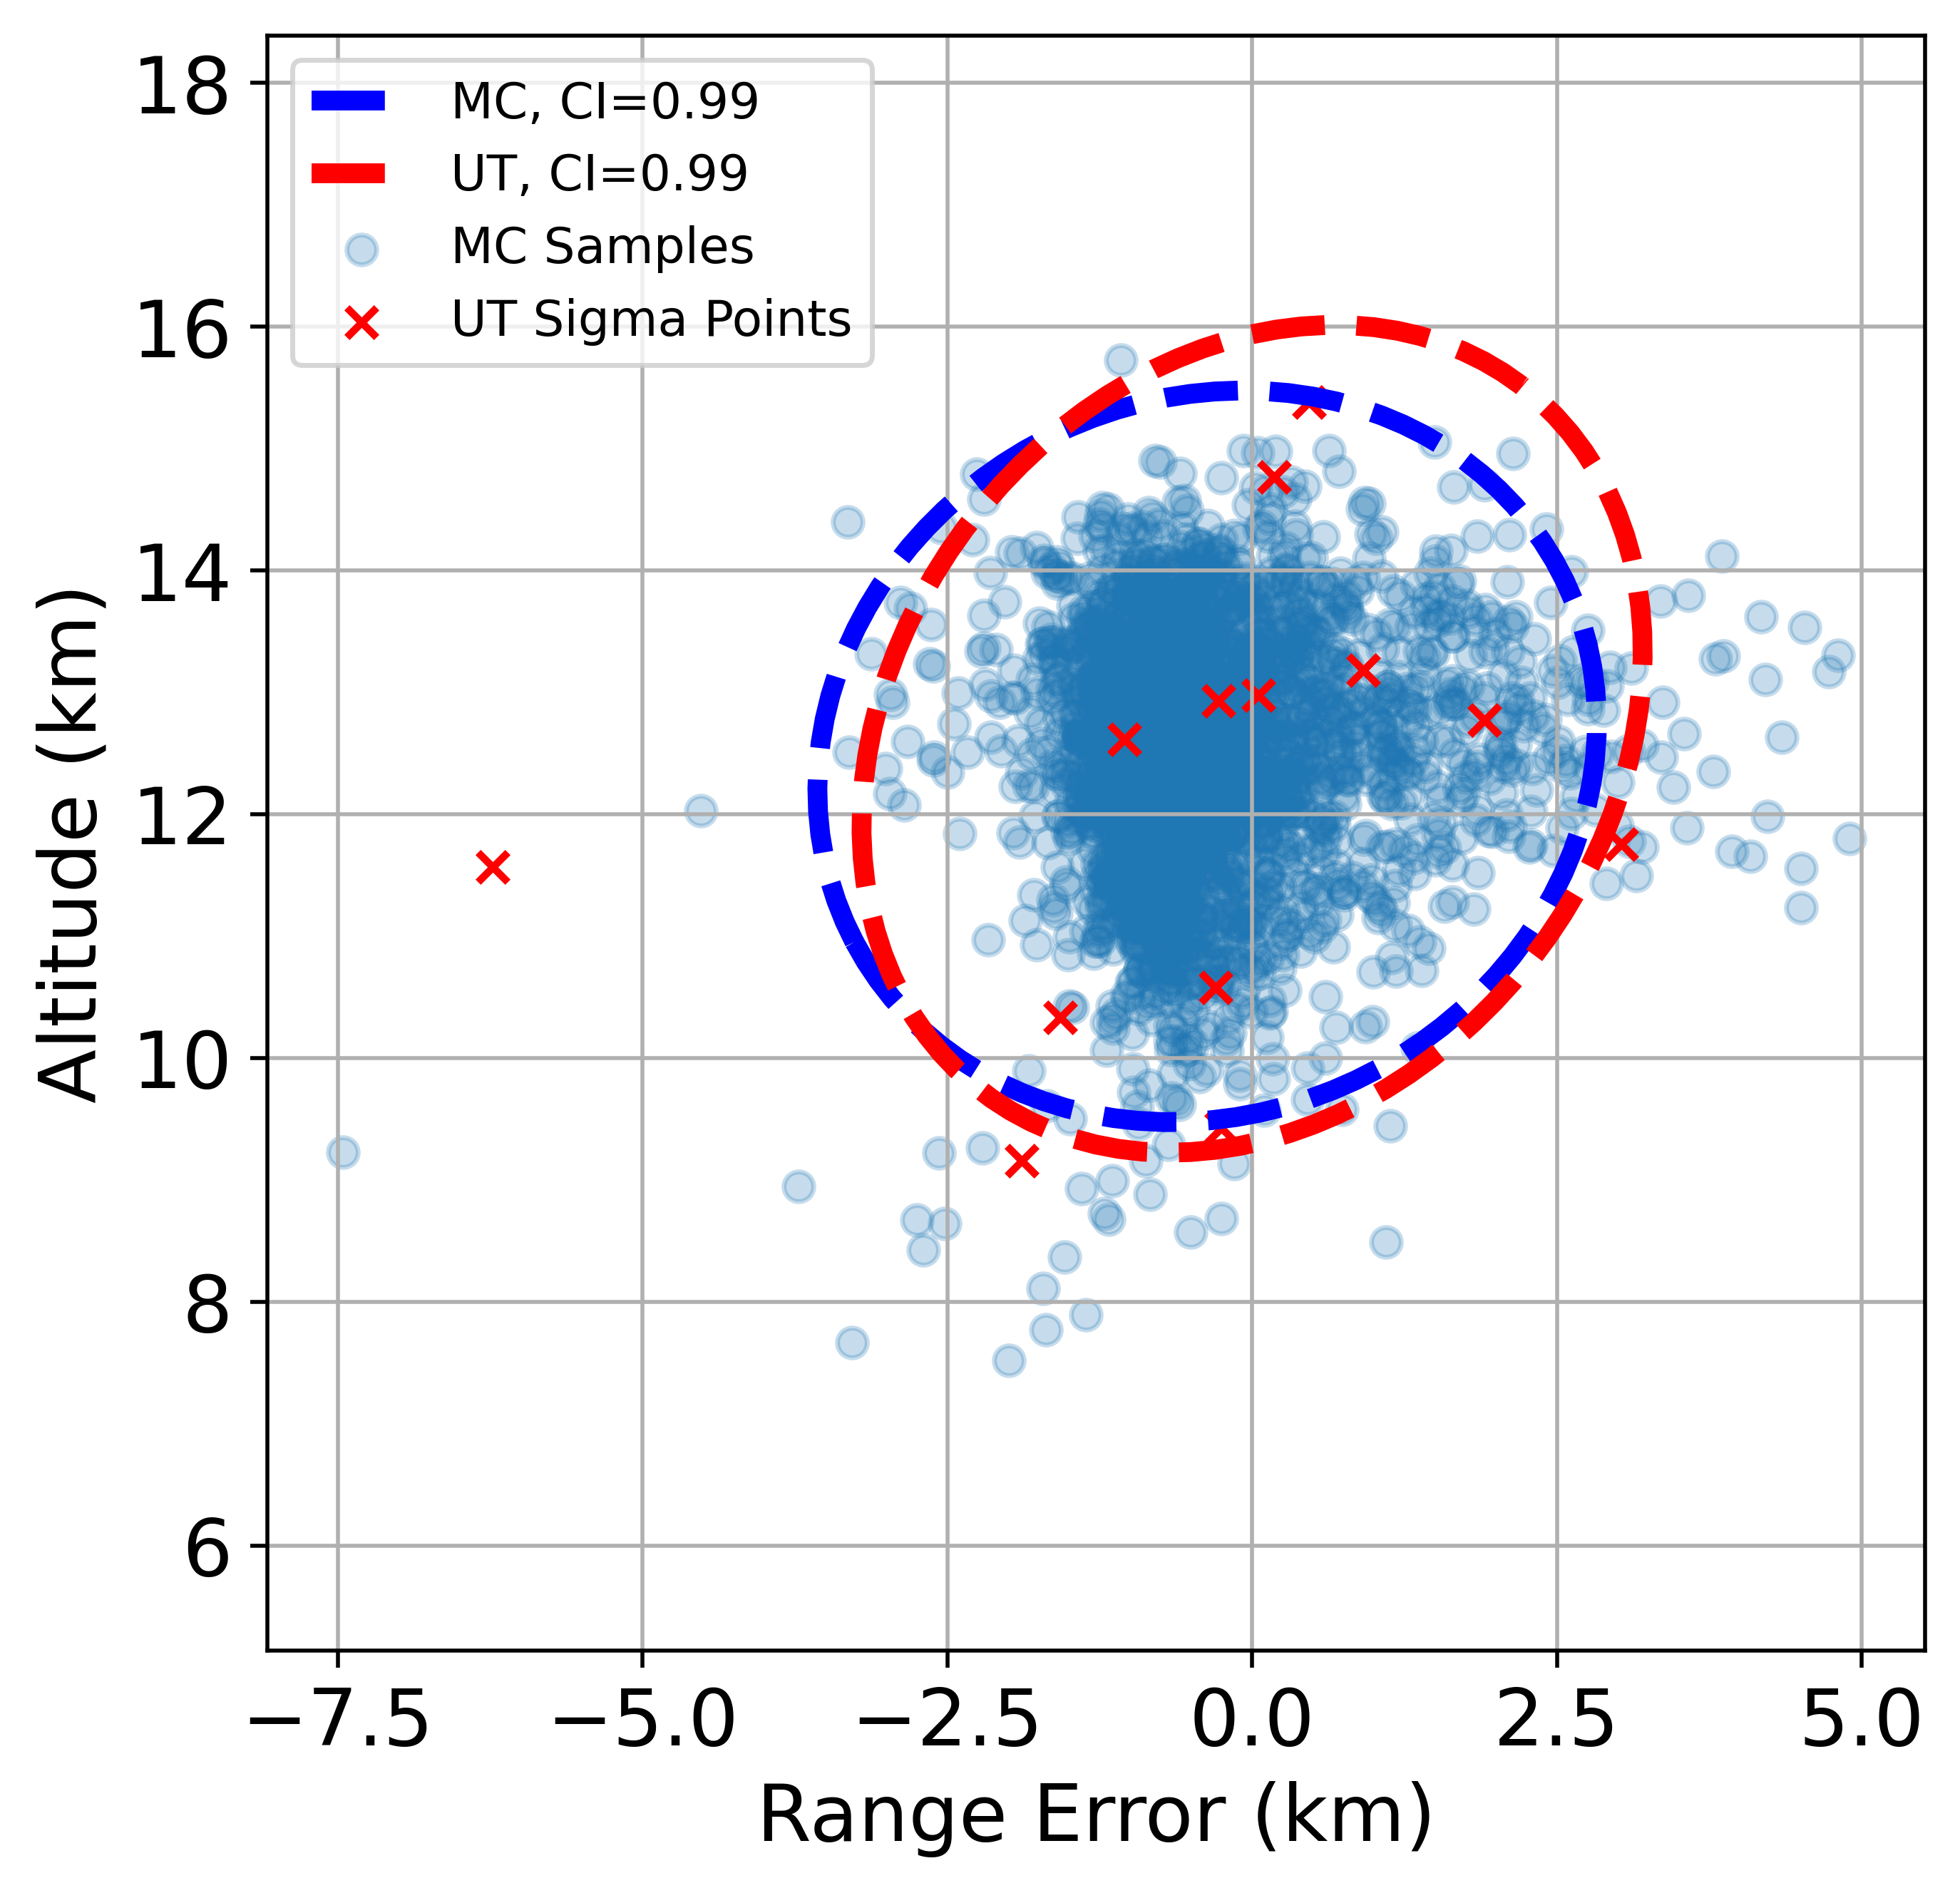
\includegraphics[width=1\textwidth]{Images/Trajectory/AltitudeRangeScatterExample}
	\caption{Terminal altitude and range performance.}
	\label{Fig:DetailedScatter}
\end{figure}
%TODO: Talk about the control saturation at the end, fragility, ability to plan for large Covariance if that's the important metric or pass/fail. 
\subsection{Sensitivity Analysis}
The numerical results show a clear tradeoff between terminal altitude and range performance. In this section we utilize MCF to determine which uncertainties are the dominant source of low altitude or high range error. MCF is a density-based, global sensitivity analysis method compatible with MC data. 

Density-based sensitivity analysis considers the PDF or CDF of an output variable, in contrast to variance-based methods that consider the second moment of the output. 
In the context of sensitivity analysis, global means to consider input variations in the entire feasible space, in contrast to local methods, like partial derivatives, that are evaluated at a single point. 

MCF proceeds as follows: given an output variable of interest, $y$, divide the MC samples into two groups based on a selected criteria. For each input variable, $x_i$, compute the ECDF of each group. Next, the the two-sample Kolmogorov–Smirnov statistic, a measure of the distance between two ECDFs, is computed as
 \begin{align}
	KS = \max_{x_i} | F_1(x_i) - F_2(x_i) | \label{Eq:KSTest}
\end{align}
where $F_i$ is the ECDF of the $i^{\mathrm{th}}$ input. Notice the the KS test is sensitive to both the shape and location of the CDF. Finally, the inputs are ranked according to their KS statistic. In our application the outputs are terminal altitude and range. For altitude, the criteria is that the sample altitude is less than the mean altitude of the samples. For range, the criteria is that the absolute error is greater than the mean absolute error. Note that the two groups do not (and need not) contain the same number of samples. Performing this test for the two different outputs and criteria are summarized in Table~\ref{Table:MCF}. The dominant sources of lower than average altitude are density and ballistic coefficient, and to a lesser extent initial errors in range and altitude. The entry flight path angle has a limited effect. Conversely, the initial state errors in altitude, range and significantly impact the guidance performance. The flight path angle and lift-to-drag ratio have a lesser effect on the range errors, and density and ballistic have little to no impact. From these results, it is clear that the uncertainties affect our quantities of interest in different ways; the only uncertainty in the top 3 of both outputs is the initial altitude. One conclusion is that in order to simultaneously achieve high altitude and low range error is to effectively mitigate all of the different sources of uncertainty. 
%TODO: Compare to MSL - I think they largely found the same thing 
% Direct quotes that should be reword:
%Density-based sensitivity indices are moment-independent indices because, by definition, they consider the entire probability distribution of the output rather than one of its moments only.
\begin{figure}[h!]
	\centering
	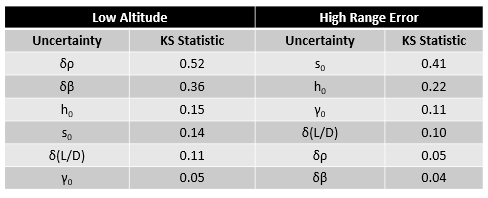
\includegraphics[width=1\textwidth]{Images/MCFTable}
	\caption{KS statistics estimating the sensitivity of terminal altitude and range to the uncertain input variables.}
	\label{Table:MCF}
\end{figure}

\section{Convergence}
In this section we examine the convergence of solutions using the full DDP algorithm, with the $\mathbf{f}_{\state\state}=\zero,\, \mathbf{f}_{\control\state}=\zero$ modification proposed in Subsection~\ref{Sec:DDP_Simplification} (labeled DDP-ControlHessian in figures), and the iterated Linear Quadratic Regulator~\cite{iLQG} (iLQR) variation where additionally $\mathbf{f}_{\control\control}=\zero$. We solve the ROGP for $w_h=w_s=1$ with each method. The primary metrics that we are interested in are the total cost, the total number of iterations, the time spent computing derivatives, and the maximum of the norm of the gradient of the value function with respect to the controls over the entire trajectory. We will also examine the linesearch stepsizes and regularization parameters. In this example, only the parametric uncertainties in ($[L/D,\beta,\rho]$) are considered; the initial state uncertainty is set to zero. The reason is that the number of sigma points, and thus the number of states in the extended state vector, depends on the uncertainty dimension. While there is no difficulty in solving the full six dimensional problem (and indeed larger sizes) using the iLQR or DDP-ControlHessian, the laptop used to solve the ROGP could not even store the full Hessian matrices for all $N=250$ steps used in the original DDP formulation.

\begin{figure}[h!]
	\centering
	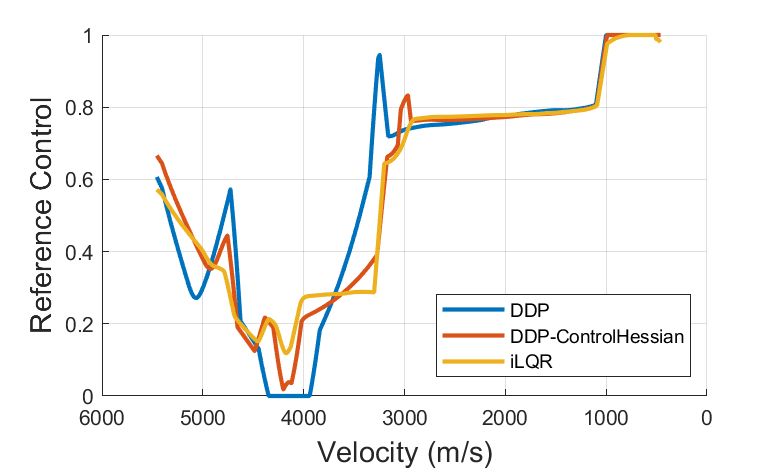
\includegraphics[width=0.75\textwidth]{Images/Convergence/ControlProfiles}
	\caption{Total cost per iteration}
	\label{Fig:ConvergeControls}
\end{figure}
\begin{figure}[h!]
	\centering
	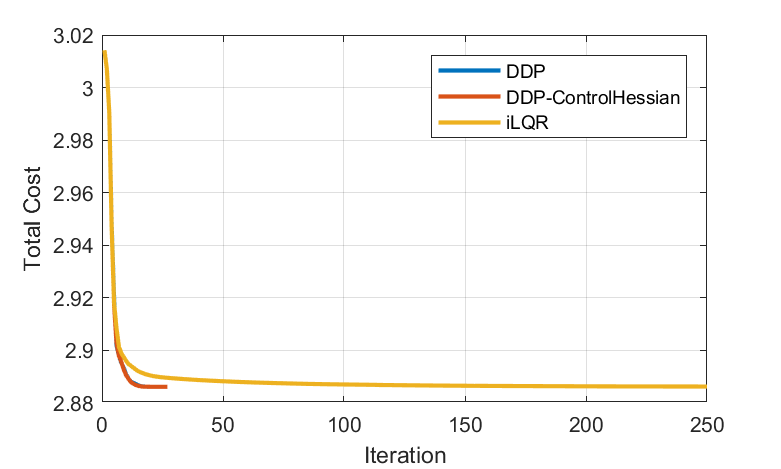
\includegraphics[width=0.75\textwidth]{Images/Convergence/cost}
	\caption{Total cost per iteration}
	\label{Fig:ConvergeCost}
\end{figure}
\begin{figure}[h!]
	\centering
	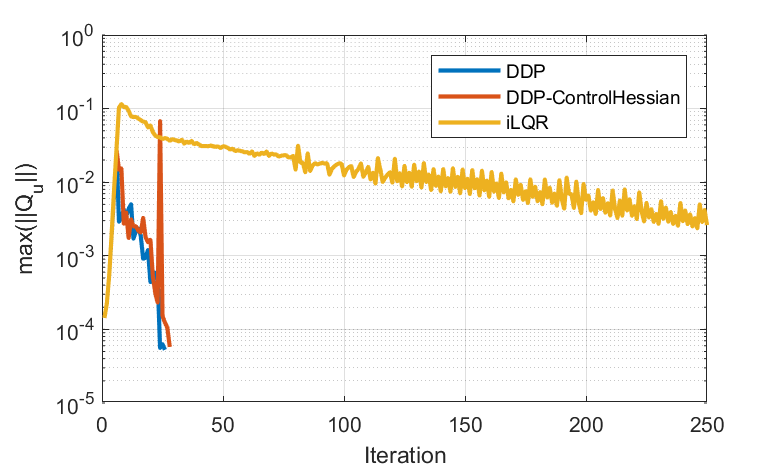
\includegraphics[width=0.75\textwidth]{Images/Convergence/grad_norm}
	\caption{Maximum control gradient norm over all timesteps.}
	\label{Fig:ConvergeGradient}
\end{figure}
\begin{figure}[h!]
	\centering
	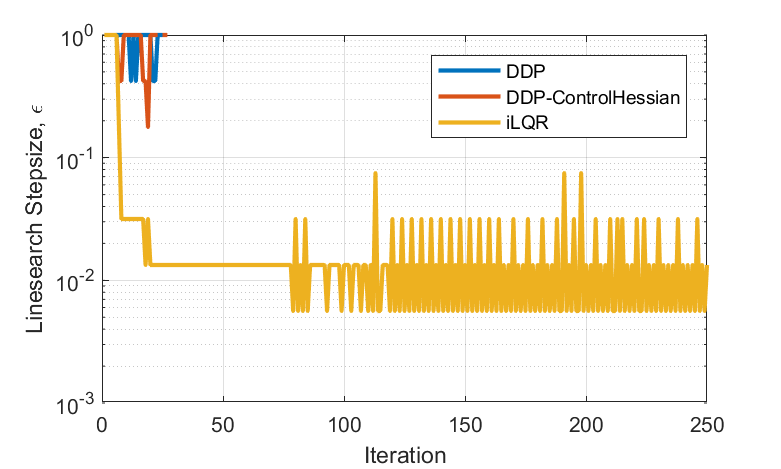
\includegraphics[width=0.75\textwidth]{Images/Convergence/alpha}
	\caption{Backtracking linesearch stepsize per iteration.}
	\label{Fig:ConvergeStepsize}
\end{figure}
\begin{figure}[h!]
	\centering
	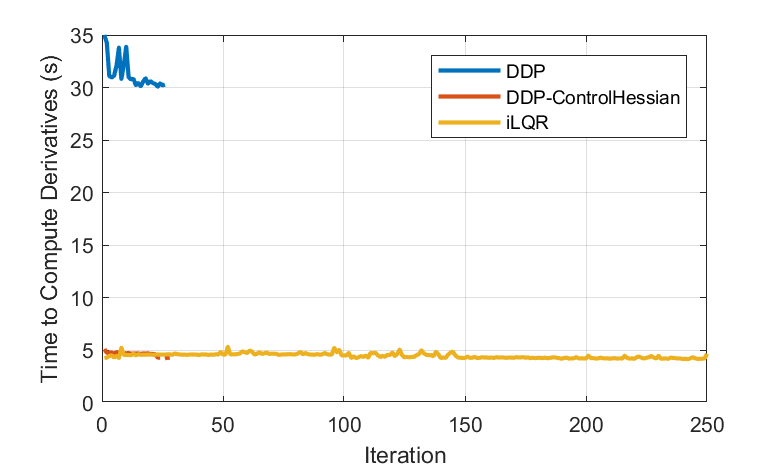
\includegraphics[width=0.75\textwidth]{Images/Convergence/time_derivs}
	\caption{Time in seconds spent computing derivatives of the cost and dynamics at each iteration.}
	\label{Fig:ConvergeTime}
\end{figure}
%TODO: SHow control profiles? All three converge to similar but not exactly the same profile. 
Figure~\ref{Fig:ConvergeControls} shows the resulting reference controls. While the results are similar, the three methods do not converge to identical solutions. 
Figure~\ref{Fig:ConvergeStepsize} shows the total cost at each iteration. Full DDP achieves the lowest cost of 2.868 after 81 iterations. Control Hessian-only DDP achieves a cost of 2.870 after 46 iterations, and iLQR has the highest cost, 2.871, and still has not terminated after 250 iterations. Figure~\ref{Fig:ConvergeGradient} shows the maximum gradient at each iteration. Unlike the DDP variants, the gradient never meets the exit criteria and thus is terminated based on the number of iterations. 
Figure~\ref{Fig:ConvergeStepsize} shows the stepsizes accepted in the linesearch procedure. Both DDP variants frequently accepted the full step $\epsilon=1$, while iLQR always took considerably smaller steps on the order of $ 10^{-2} $. Finally, Fig.~\ref{Fig:ConvergeTime} shows the drastic, nearly 10x reduction in time spent computing the derivatives resulting from omitting Hessian terms. The average times were $47.7$ s, 5.6 s, and 5.2 s, respectively. 
This example shows that, for this problem, retaining the second order derivatives with respect to the controls achieves nearly the same convergence as the full DDP algorithm while being only mildly more expensive to compute than the iLQR solution. 

%TODO: sensitivity to initial guess? 

%\section{Joint Optimization of Velocity-Varying Gains}
%Show negative result and describe overfitting problem. 

%\section{As Vehicle Design Tool}
%What L/D is required to achieve similar entry altitudes for a heavier vehicle of $\beta=200$? We use a simple scaling of the L/D profile $L/D$. The gains are jointly optimized, and additionally, the entry flight path angle is treated as a design variable. To estimate a useful lower bound on the L/D, we select $w_h=3, w_s=0$; the desired solution will likely place non-zero weight on the range errors, and thus need even more L/D. 
%%% Local Variables: ***
%%% mode: latex ***
%%% TeX-master: "thesis.tex" ***
%%% End: ***

\chapter{Sample Retrieval Lander Class Assessment}\label{Ch:SRL_EDL}
%TODO: Massage paper results into here. A key result is the altitude performance; can't reach all altitudes that MSL/M2020 could (up to -1 km), but it can reach altitudes where MSL is, not sure what altitude M2020 is (but that's where its going). 
In Ref.~\cite{MyRobustOCPaper}, an earlier version of the work in the dissertation, we assessed the robust optimal guidance on a vehicle in the class of the Sample Retrieval Lander (SRL) mission of the Mars Sample Return campaign\cite{MSR,MSR2}. The ballistic coefficient of the vehicle is 200 $ \mathrm{kg/m}^2 $ with an entry mass of 5000 kg. In order to contend with the increased ballistic coefficient, the vehicle L/D is raised to 0.28 (assumed to be constant, in contrast to the earlier results for the MSL-class vehicle). The same state and uncertainty at the entry interface presented in Chapter~\ref{Ch:AssessmentConditions} are assumed. The resulting mean entry state is $x_0 = [54.5\,\mathrm{km},\,-11.5^{\circ}, 0\,\mathrm{km}]^T$ at $v_0 = 5525$ m/s. The same parametric uncertainty is considered except the altitude-varying Mars Climate Database model is replaced with a constant fractional offset with $3\sigma_{\rho} = 20$\%. In this earlier work, we had not yet developed the DDP extension to jointly optimize the static feedback gains presented in Section~\ref{Sec:DesignOptimization}. As a result, any feedback gain optimization presented in this chapter was performed separately from the reference control using a sequential quadratic programming method to minimize the original terminal objective in Eq.~\eqref{Eq:Objective}, as estimated using the UT.

In the first section, the unscented transform is used to estimate the performance of an unguided entry vehicle to determine the magnitude of errors that must be mitigated by the entry guidance. In the second section, reference trajectories and controls generated by our approach are compared to those designed by nominal optimal control with fixed bank angle margins. By nominal optimal control we refer to the optimization of a single trajectory without considering uncertainty and closed-loop guidance. The third section investigates how the optimal trajectories change with the weights $w_h$ and $w_s$, incorporating both initial state uncertainty and parametric uncertainty. The final subsection presents a detailed look at one solution and the corresponding Monte Carlo statistics.

\section{Open-Loop Simulation}
\begin{figure}[h!]
	\centering
	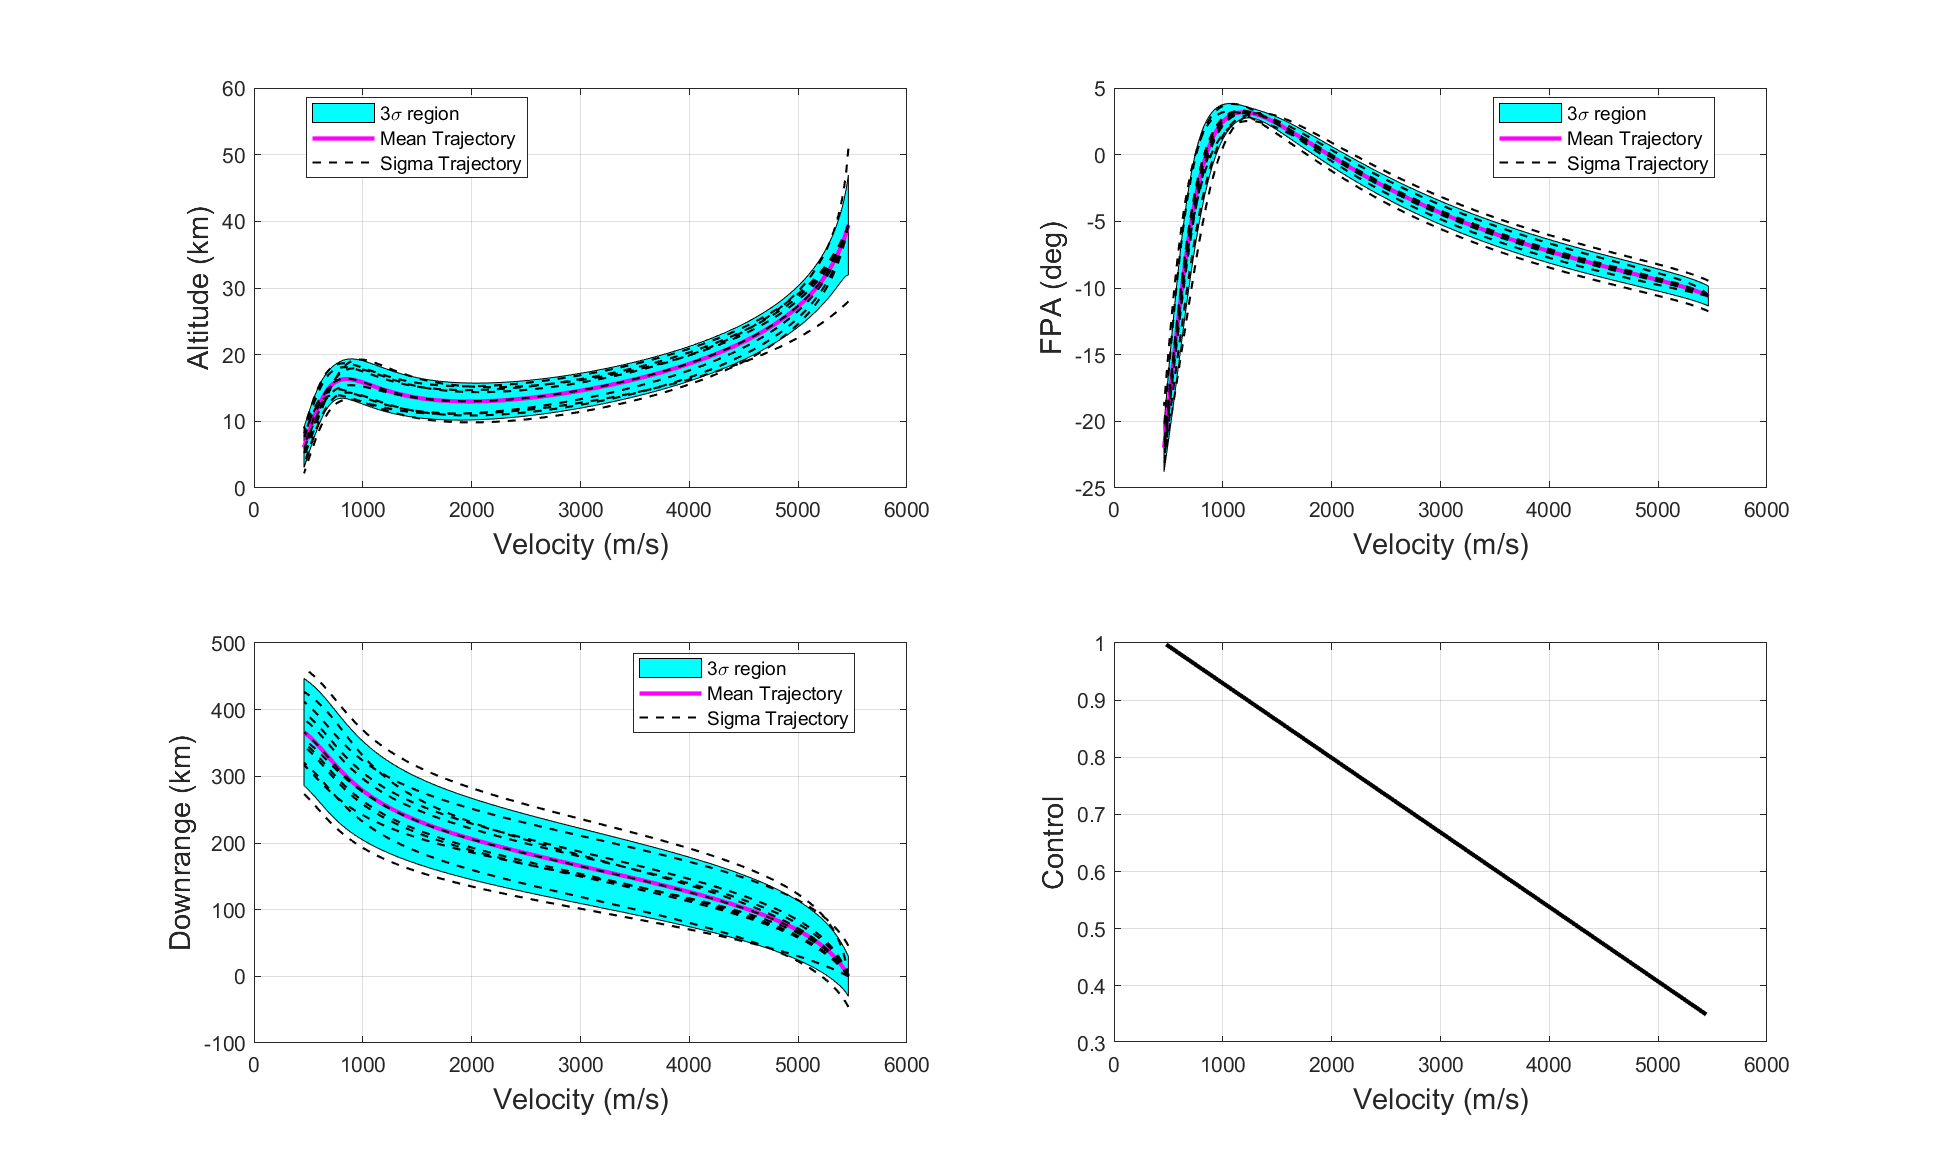
\includegraphics[width=1\textwidth]{../PropellantOptimalJournal/ddp/matlab/HeavyOpenLoopGrid}
	\caption{The sigma point trajectories for an unguided entry trajectory.}
	\label{Fig:OpenLoop}
\end{figure}
In order to estimate the magnitude of the range and altitude dispersions that must be mitigated by the guidance commands, we simulate the performance of our initial trajectory with the feedback gains set to zero. Since the purpose of determining the magnitude of the terminal errors is as a point of reference, the unscented transform estimate is used rather than full Monte Carlo simulation. The altitude, range, FPA, and nominal control profiles are shown in Fig.~\ref{Fig:OpenLoop}, including the sigma point trajectories and the UT-estimated 3$\sigma$ region. The control profile, shown in the bottom right of the figure, is a linear ramp from $u(v_0)=0.35$ to $ u(v_f)=1 $. The mean altitude is 6.08 km and the 3$\sigma$-low altitude is 3.09 km. At the chute deploy velocity, 460 m/s, the target range is 366.4 km and the 3$\sigma$ range error is $80.3$ km. Thus the robust optimal guidance has substantial potential errors to overcome.

\section{Reference Trajectory Comparison}
In this subsection we compare the performance of the robust optimal guidance using six different reference trajectory-control pairs. For all six cases, the control law in Eq.~(\ref{Eq:Control}) is used with the same feedback gains and feedback control limits, Eq.~(\ref{Eq:Control_bounds}). In the first three cases, a reference trajectory and control are generated by solving the optimal control problem $\min J = -h(v_f)$ subject to nominal longitudinal dynamics with different limits on the reference control to preserve margin for feedback. For the remaining three cases, the solution to the ROGP is used to generate the reference trajectory and control. Monte Carlo simulations are used to assess the guidance performance.

Case 1 considers $u_{\mathrm{ref}}\in[0,1] = [\cos90^{\circ},\cos0^{\circ}]$, Case 2 considers $u_{\mathrm{ref}}\in [\cos75^{\circ},\cos15^{\circ}]$, and Case 3 considers $u_{\mathrm{ref}}\in [\cos60^{\circ},\cos30^{\circ}]$.
Bank angle margin is important for range control, as well as for preserving control authority for lateral guidance, which is not modeled here. 
Cases 4-6 solve the robust optimal guidance problem with different choices of the weights to design the reference trajectories. Case 4 optimizes mean altitude ($ w_h=w_s=0 $), Case 5 optimizes the 3$\sigma$-low altitude ($ w_h=3,\,w_s=0 $), and Case 6 optimizes a combination of mean altitude and 3$\sigma$ downrange deviation ($ w_h=0, w_s=3 $). Recall that each of the six cases may achieve a different downrange distance.

The feedback gains are constants $[k_D, k_{\gamma}, k_s] = [0.0725, -0.025, -0.004]$.  These gains were computed by minimizing the UT-estimated downrange distance standard deviation for the initial guess at the control profile, which is a linear (in velocity) ramp from zero to one. Different initial guesses for the optimal profile would yield some variation in these gains, and superior results can be obtained by optimizing the gains for each solution, but using the same gains for all of the cases allows us to highlight the impact of the reference trajectory without confounding variables. These gains are used in the optimization process for Cases 4-6, and in the Monte Carlo simulations for all six cases. 

\begin{figure}[h!]
	\centering
	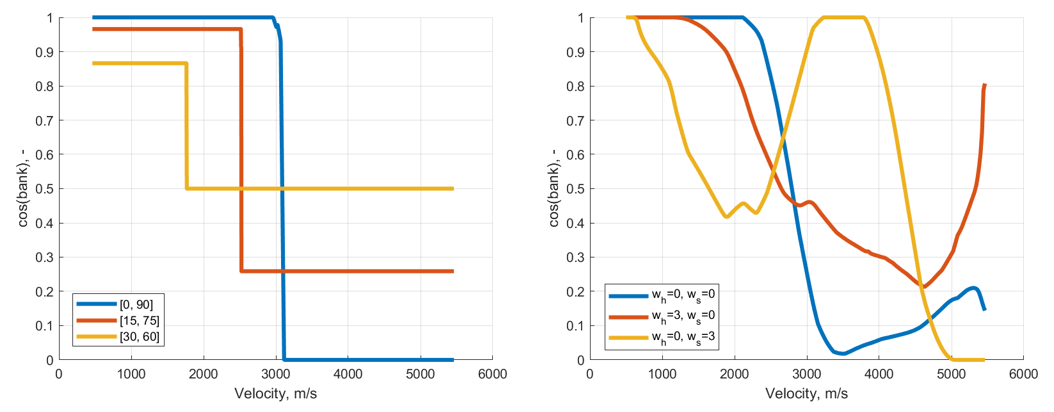
\includegraphics[width=1\textwidth]{../PropellantOptimalJournal/ddp/comparison_controls}
	\caption{The profiles from deterministic optimal control (left) exhibit the well known bang-bang structure of altitude optimal trajectories. In comparison, the robust control histories (right) exhibit significantly different behavior depending on the weights applied.}
	\label{fig_control_comparison}
\end{figure}

Figure~\ref{fig_control_comparison} shows the resulting control profiles for the six cases. The altitude-optimal controls resulting from nominal optimal control (Cases 1-3) exhibit the well-known bang-bang structure, while the robust optimal control profiles are quite varied depending on the weights selected. For Case 4, which optimizes mean altitude, the profile is somewhat similar to the bang-bang profiles, but retains margin at high velocities and has a slower transition to a lift up ($u=1$) orientation. An interesting feature of the robust profiles is that they exhibit significant margins, as solutions to the problem that considers robustness. Nevertheless, saturation still occurs at some velocities. This suggests that the robust optimal amount of margin varies along the trajectory, which implies using a fixed margin will produce inferior results, as the results presented next indicate. Although lateral guidance control authority ($L/D \sin\sigma$) is not considered in the formulation of the robust performance optimization problem, the solutions show that there is significant, though non-uniform, margin. Further consideration of compatibility with lateral guidance is left for future work. 

%TODO: Add a note that the target downrange distance is different for each Case.

The results are summarized in Tables~\ref{table_deterministic}-\ref{table_robust}. Case 1 preserves no margin at all, and as a result has the highest nominal terminal altitude of the three cases. This translates into the highest mean altitude of the three cases, despite the lack of margin. However, the lack of margin causes poor range control performance in many trajectories, leading to large mean and 3$\sigma$ range errors. While the mean error can be reduced by target biasing, the 3$\sigma$ range error is the largest of the 6 cases. As the amount of control margin increases in Cases 2 and 3, both the mean and 3$\sigma$ range errors drop dramatically while the mean altitude also decreases. The 3$\sigma$-low altitudes display non-monotonic behavior with respect to bank margin because the mean altitude loss may or may not be offset by the reduction in altitude deviation. This is true for Case 2, which has a higher 3$\sigma$-low altitude relative to Case 1. In Case 3, the drop in mean altitude is greater than the drop in the 3$\sigma$-low altitude because the altitude deviation has decreased further. 

Case 4 ($ w_h=w_s=0 $) optimizes the mean altitude with knowledge of the problem uncertainty and guidance gains. The mean altitude is 50 m lower than Case 1 because the UT overestimated the mean. However, this difference is quite small, and the performance is more robust because the 3$\sigma$-low altitude is higher and the 3$\sigma$ range error is smaller. Case 5 ($ w_h=3,w_s=0 $) adds additional weight to the altitude standard deviations, resulting in a 500 m increase to the 3$\sigma$-low altitude despite a 300 meter drop in mean altitude relative to Case 4. Case 5 has the highest 3$\sigma$-low altitude of the six cases, with a 200 m increase over the best of the three profiles designed without considering uncertainty. Case 6 ($ w_h=0, w_s=3$) places no weight on altitude standard deviation, but weights range errors heavily, and produces a 1.5 km decrease in 3$\sigma$ range errors as a result. It has the lowest range error of the six cases, and compared to the large margins of Case 3, still produces a higher 3$\sigma$-low altitude.

This demonstrates the benefit of robust optimal control to designing reference trajectories. Additionally, the flexibility of the weights allows the trajectory designer to trade between range errors and altitude performance to the extent that the reference trajectory can alter closed-loop performance. 
\begin{table}[h!]
	\centering
	\caption{Monte Carlo statistics for cases 1-3, with reference trajectories designed using optimal control and fixed bank margins.}
	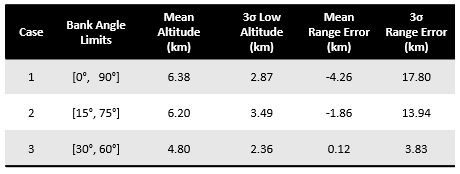
\includegraphics[width=0.65\textwidth]{../PropellantOptimalJournal/ddp/table_deterministic}
	\label{table_deterministic}
\end{table}
\begin{table}[h!]
	\centering
	\caption{The Monte Carlo statistics for cases 4-6, with reference trajectories designed using the proposed method.}
	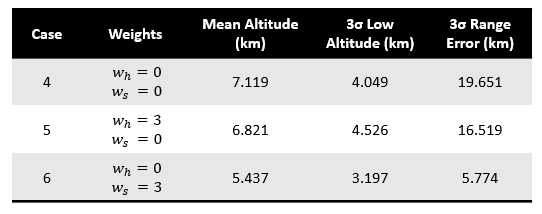
\includegraphics[width=0.65\textwidth]{../PropellantOptimalJournal/ddp/table_robust} %
	\label{table_robust}
\end{table}
%Figures~\ref{fig_robust_alt}-\ref{fig_robust_range} show the estimated $3\sigma$ deviations around the mean as well as the sigma point trajectories for scenario 1.
%\begin{figure}[h!]
%	\centering
%	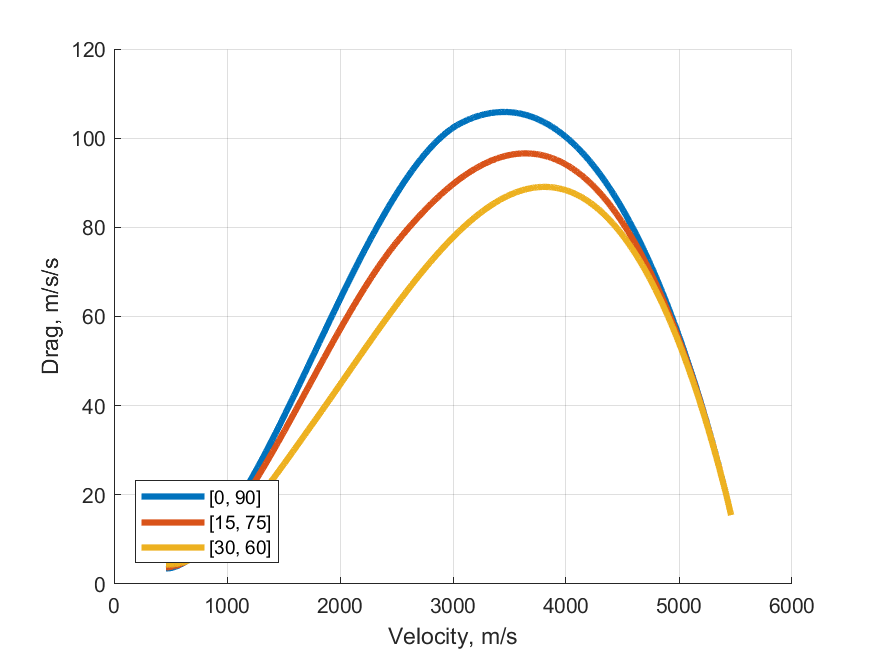
\includegraphics[width=1\textwidth]{ddp/matlab/NominalDrag}
%	\caption{Reference drag profile for each of the four scenarios in Table~\ref{table_comparison}.}
%	\label{fig_drag}
%\end{figure}
%\begin{figure}[h!]
%	\centering
%	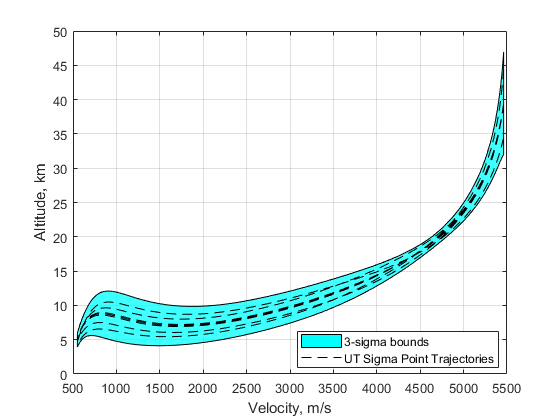
\includegraphics[width=1\textwidth]{ddp/matlab/RobustTrajAlt}
%	\caption{Dispersed altitude performance for scenario 1.}
%	\label{fig_robust_alt}
%\end{figure}
%\begin{figure}[h!]
%	\centering
%	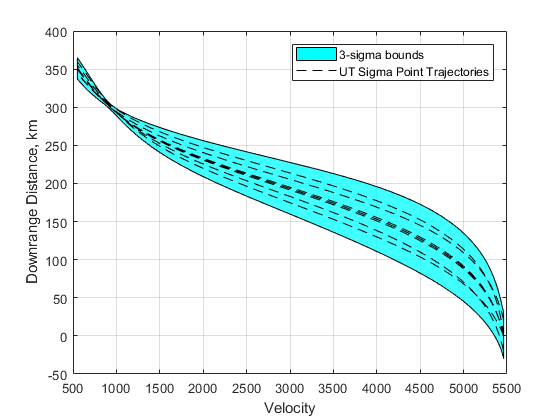
\includegraphics[width=1\textwidth]{ddp/matlab/RobustTrajRange}
%	\caption{Dispersed range performance for scenario 1.}
%	\label{fig_robust_range}
%\end{figure}


\section{Standard Deviation Weighting Design Trade}
%TODO: Double check these numbers, they may have changed 
From the previous subsection it is evident there exists a design space where weights on deviations produce superior results to simply optimizing the mean altitude when tail behavior of the distribution is important. This section investigates the extent to which weighting the standard deviations can alter the trajectory performance. The robust optimal control problem is solved for a variety of weights. The results are summarized in Fig.~\ref{fig_weight_sweep}. Again the advantages of weighting the standard deviations compared with optimizing only the mean are made clear. Comparing $w_h=w_s=0$ with, e.g., $w_h=1,\,w_s = 1$ demonstrates that a 50\% reduction in the standard deviation of downrange distance can be obtained with no loss in the low end of the terminal altitude distribution. Additionally, we can numerically determine the trade between terminal altitude and downrange robustness. The minimum downrange standard deviation achieved ($w_h=1,w_s=3$) was 0.7 km, an 85\% reduction from the mean optimization with $\sigma_s(v_f)=5.1$ km. These trajectories show clear improvements with no change to the guidance gains - simply a different reference trajectory is used to improve the results. The downrange distance shows only small improvement for weights $w_s>1$, but the low altitude continues to drop as this weight is increased. Thus, a compromise such as $w_h=w_s=1$ strikes a good balance between the two objectives. 
\begin{figure}[h!]
	\centering
	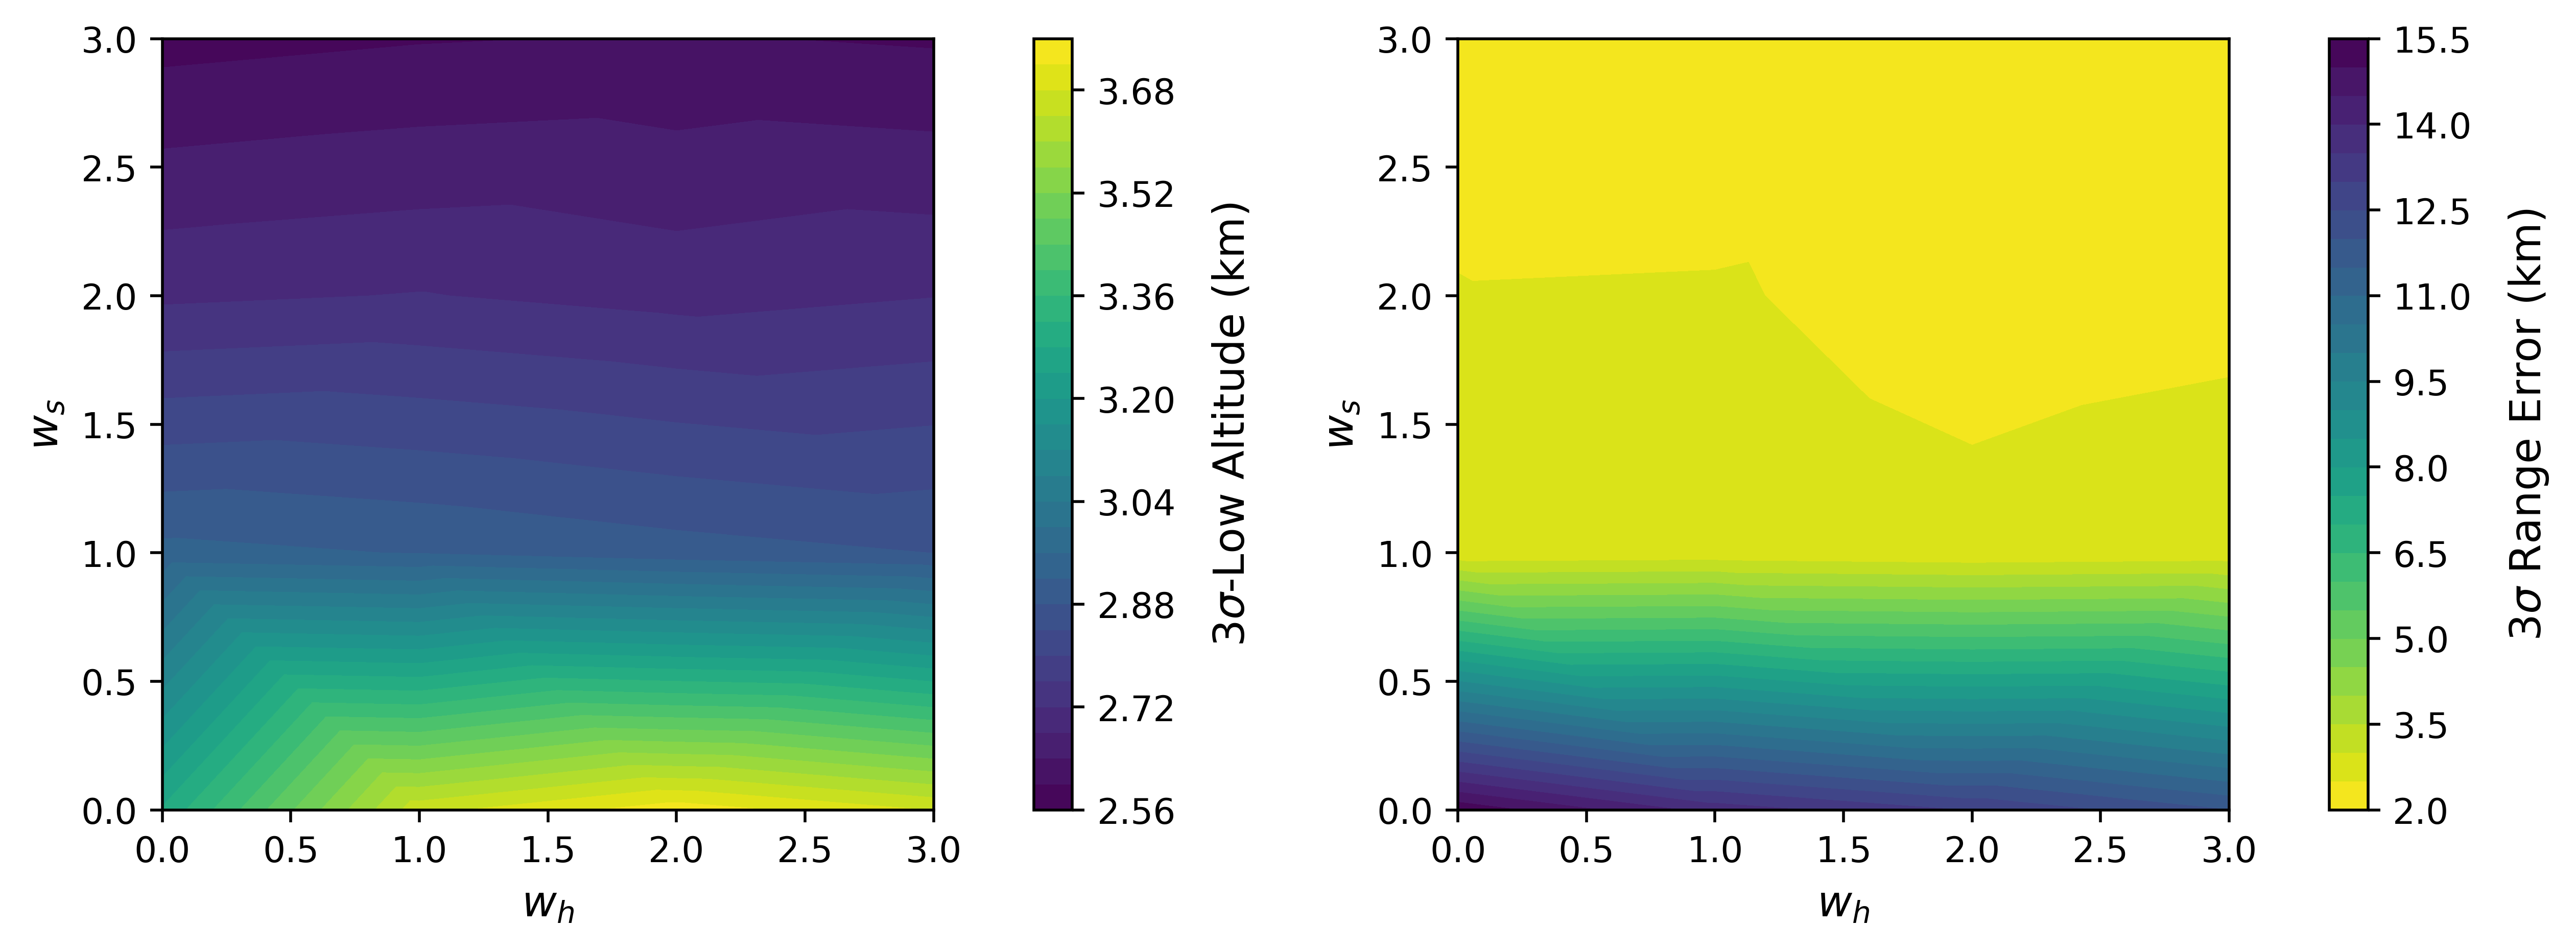
\includegraphics[width=1\textwidth]{../PropellantOptimalJournal/ddp/python/Heavy_WeightSweepMCResults}
	\caption{Contours of the Monte Carlo 3$\sigma$-low altitude (left) and 3$\sigma$ downrange distance error (right) as a function of the weights $w_h$ and $w_s$.}
	\label{fig_weight_sweep}
\end{figure}

These results also show some inaccuracy due to using the unscented transform. The 3$\sigma$-low altitude should be maximized when the objective function is exactly this quantity, i.e., $w_h=3,\,w_s=0$, but due to small estimation errors this is not the case, and the highest 3$\sigma$-low altitude is achieved with $w_h=2,\,w_s=0$. Similarly, the 3$\sigma$ range error is not minimized when $w_h=0,\,w_s=3$, but instead $w_h=1,\,w_s=3$. However, the difference in each of these cases is quite small. This issue is related to that fact that a constant UT scaling parameter $\alpha=15$ is used in all computations. Our experience with the numerical results suggests that the optimal value of $\alpha$ depends on the weights selected, and larger weights should use a higher $\alpha$. 
%Nevertheless, the solutions at all weight values are acceptable
%This also highlights the power of the approach as a design tool. If, for example, the $3\sigma$-low terminal altitude is not sufficient for any values of $w_h,\,w_s$, then some aspect of the mission must be reconsidered: increase the terminal velocity, increase the vehicle $L/D$, decrease ballistic coefficient, etc. If a $3\sigma$-low altitude limit is known, then only points that satisfy this limit are considered, and the point with the lowest downrange error may be selected. 

These results used constant feedback gains, so it is likely that methods of generating gains that vary along the trajectory, such as the Linear-Quadratic Regulator, Apollo influence coefficients \cite{Apollo}, or joint optimization of the feedback gains in the robust optimal control problem, could produce even greater synergistic improvements to the trajectory design. Additionally, the constant feedback gains were optimized for the initial guess trajectory, so further improvement is possible by reoptimizing the gains for the converged trajectory and control, as will be done in the following subsection.

\section{Comparison of UT and Monte Carlo Statistics}
The previous subsections looked at broader trends when using the proposed method to design reference trajectories. This subsection will focus on a single solution, and compare the UT and Monte Carlo statistics in greater detail. Additionally, the feedback gains are again constants, but for this case they are reoptimized to minimize UT-estimated downrange errors after finding the optimal reference control with the previous gains. The reoptimized gains are $[k_D, k_{\gamma}, k_s] = [0.058, -0.021, -0.005]$. Since each component of the objective is important and a compromise must be met, we select the weights $w_h=w_s=1$. A Monte Carlo simulation is conducted with 8000 samples in order generate precise statistics for comparison with the unscented transform. 
\begin{table}[h!]
	\centering
	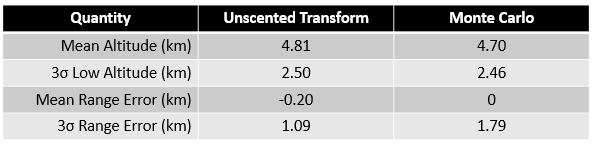
\includegraphics[width=0.75\textwidth]{../PropellantOptimalJournal/ddp/table_mc}
	\caption{Summary of the statistics from the Unscented Transform and Monte Carlo}
	\label{table_mc}
\end{table}
\begin{figure}[h!]
	\centering
	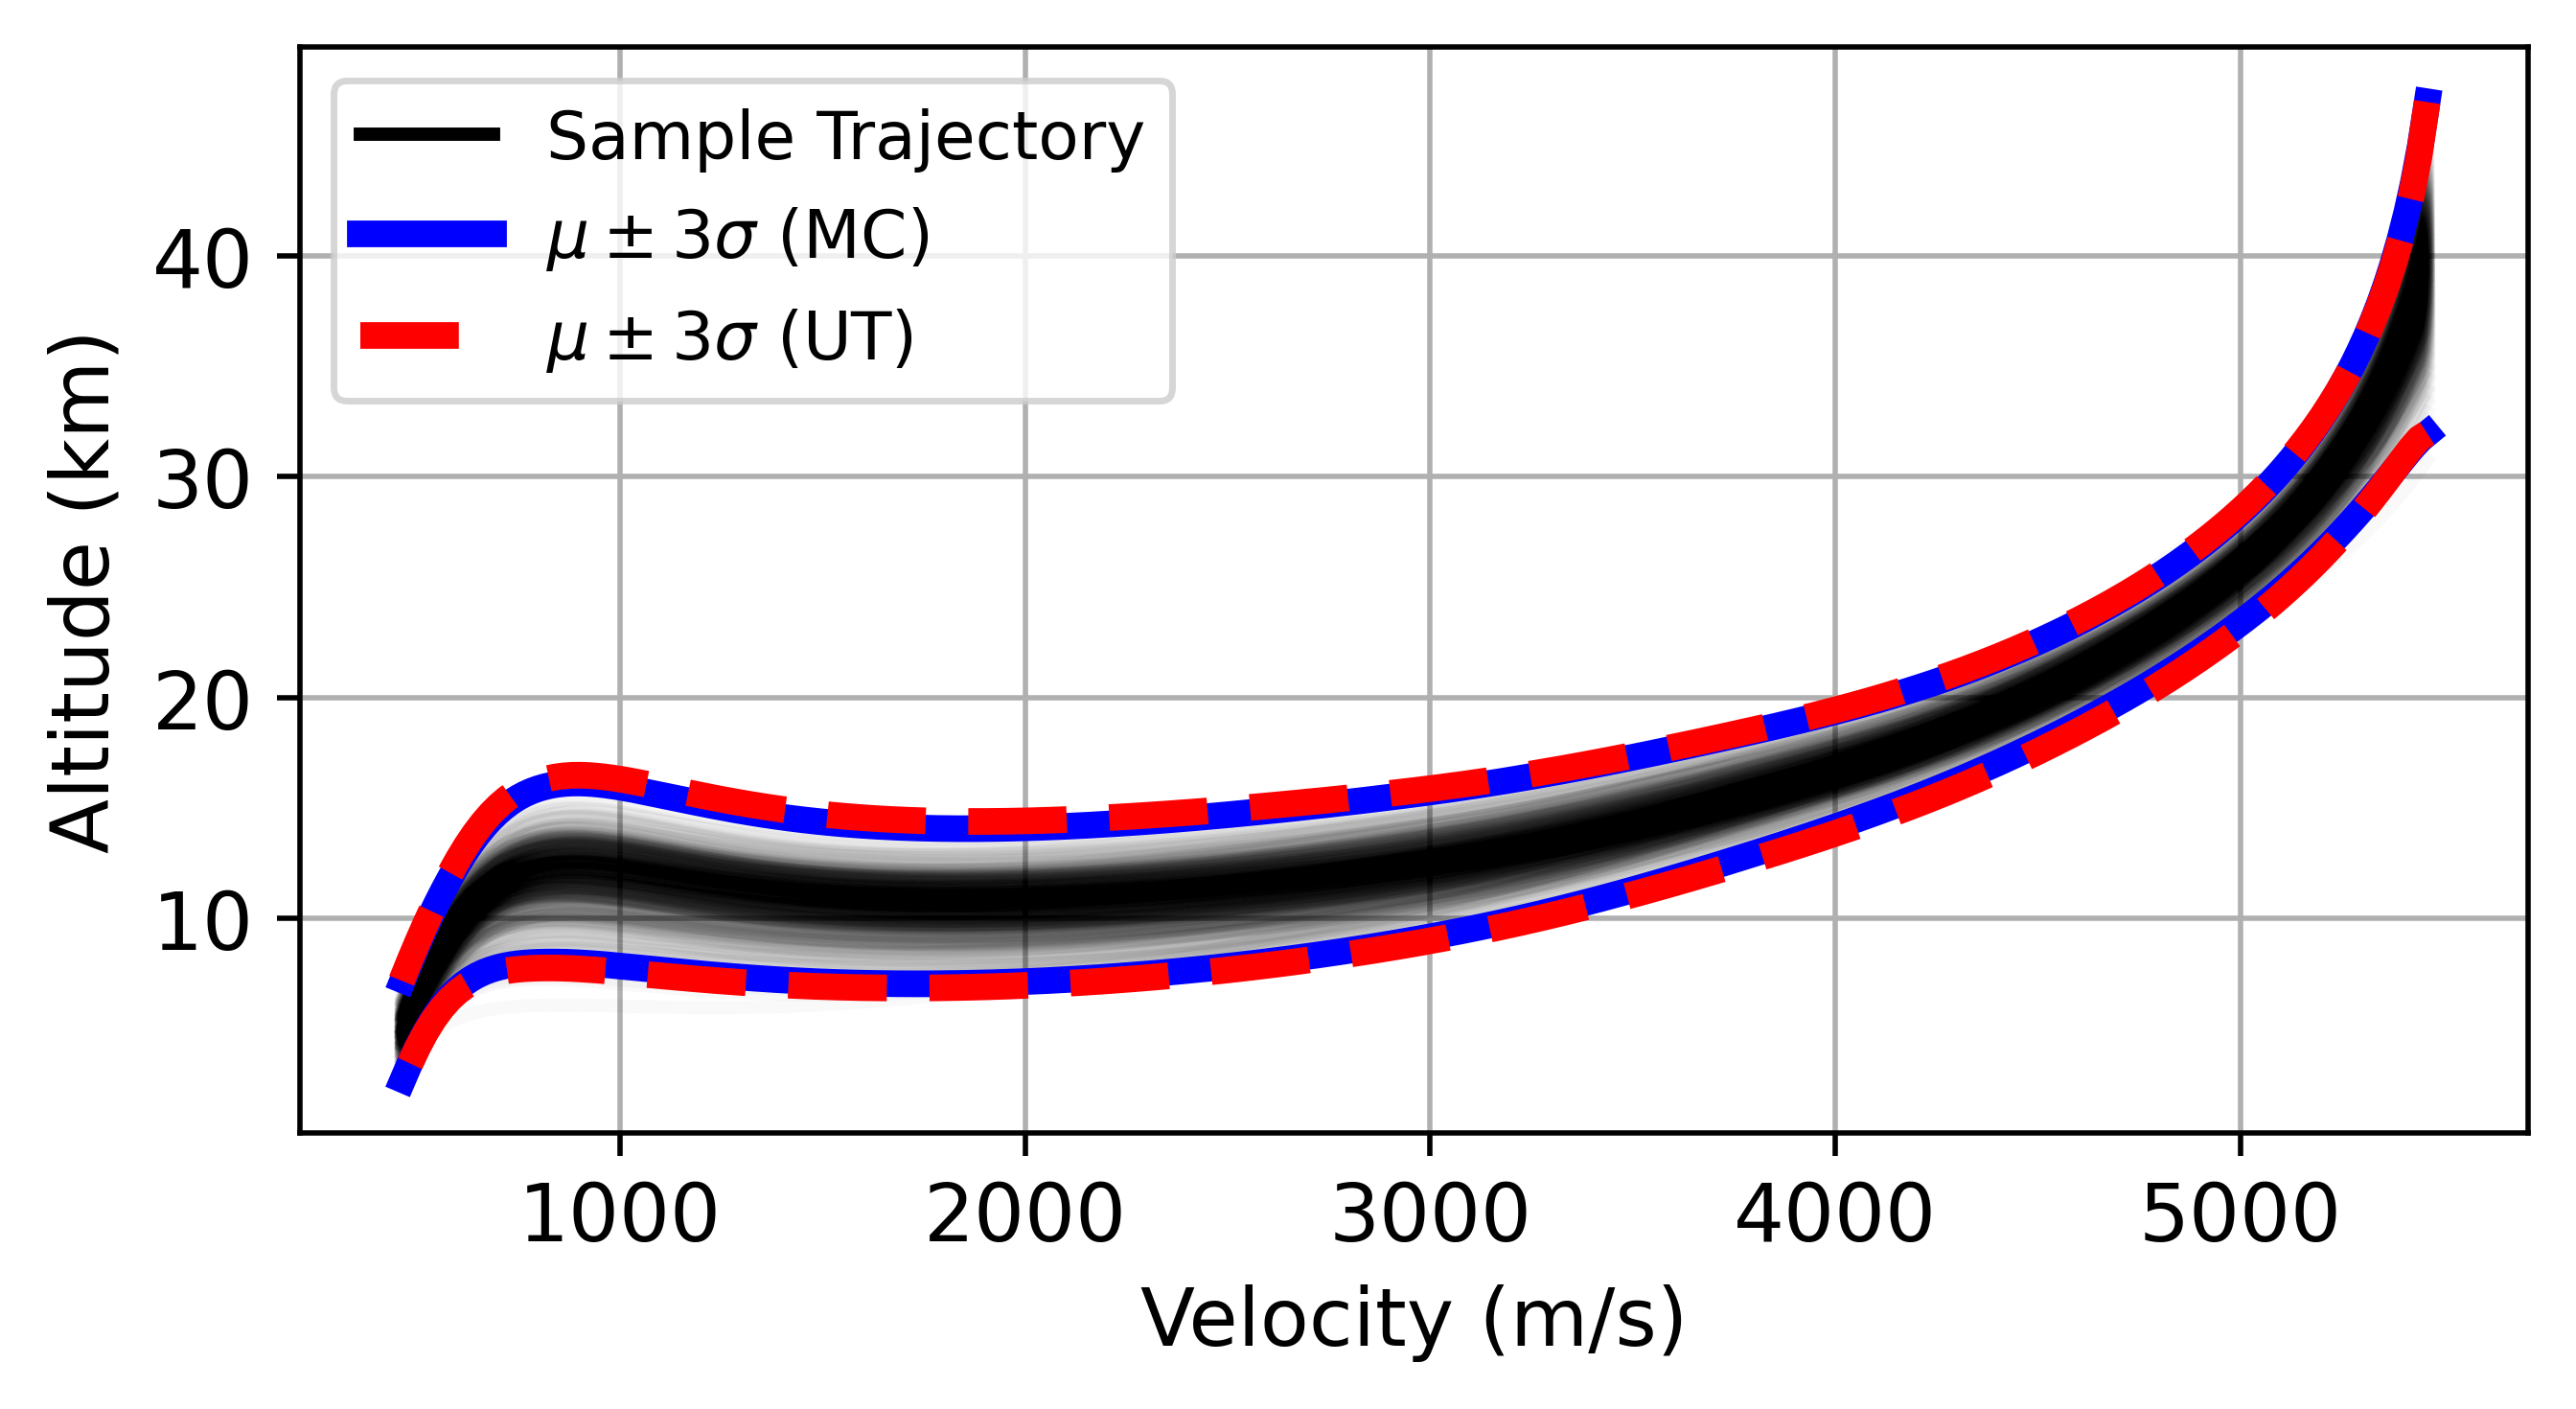
\includegraphics[width=0.75\textwidth]{../PropellantOptimalJournal/ddp/python/Altitude}
	\caption{Altitude versus velocity for 500 sample trajectories with Monte Carlo- and UT-estimated 3$\sigma$ bounds. The 3$ \sigma $-low altitude is 2.5 km.}
	\label{fig_mc_alt}
\end{figure}
\begin{figure}[h!]
	\centering
	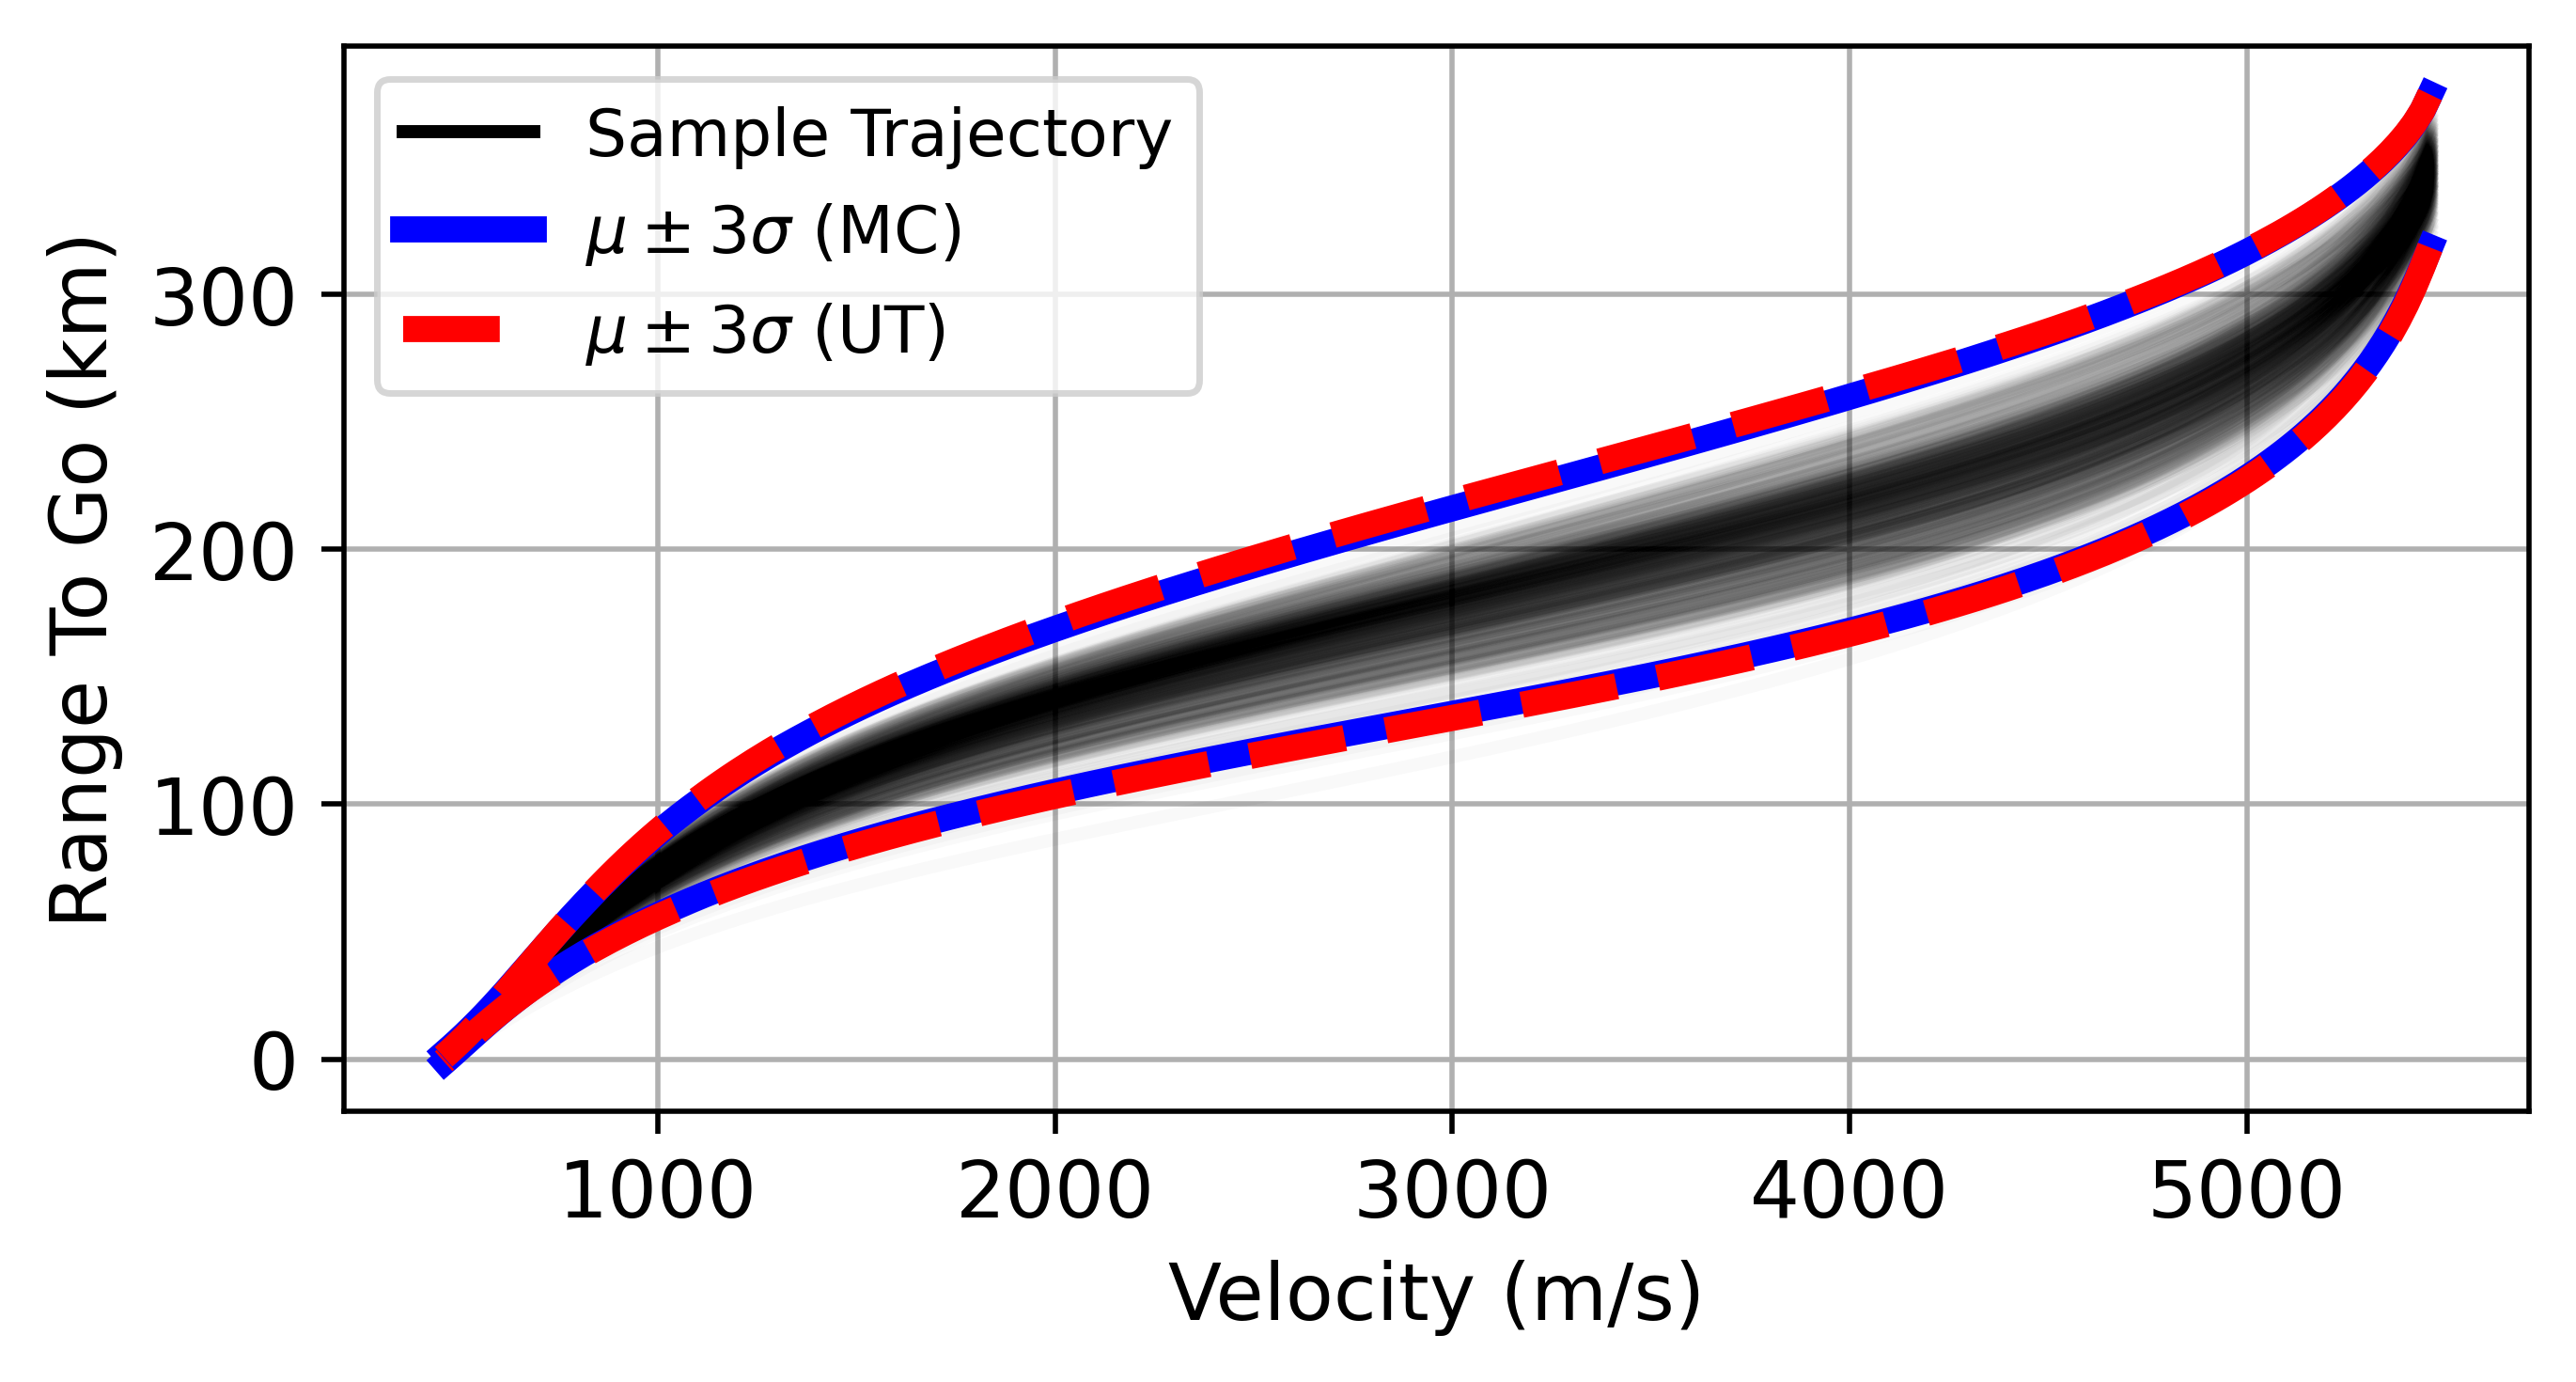
\includegraphics[width=0.75\textwidth]{../PropellantOptimalJournal/ddp/python/Range}
	\caption{Range to go versus velocity for 500 sample trajectories with Monte Carlo- and UT-estimated 3$\sigma$ bounds. The terminal 3$ \sigma $ range error is 1.8 km.}
	\label{fig_mc_range}
\end{figure}
\begin{figure}[h!]
	\centering
	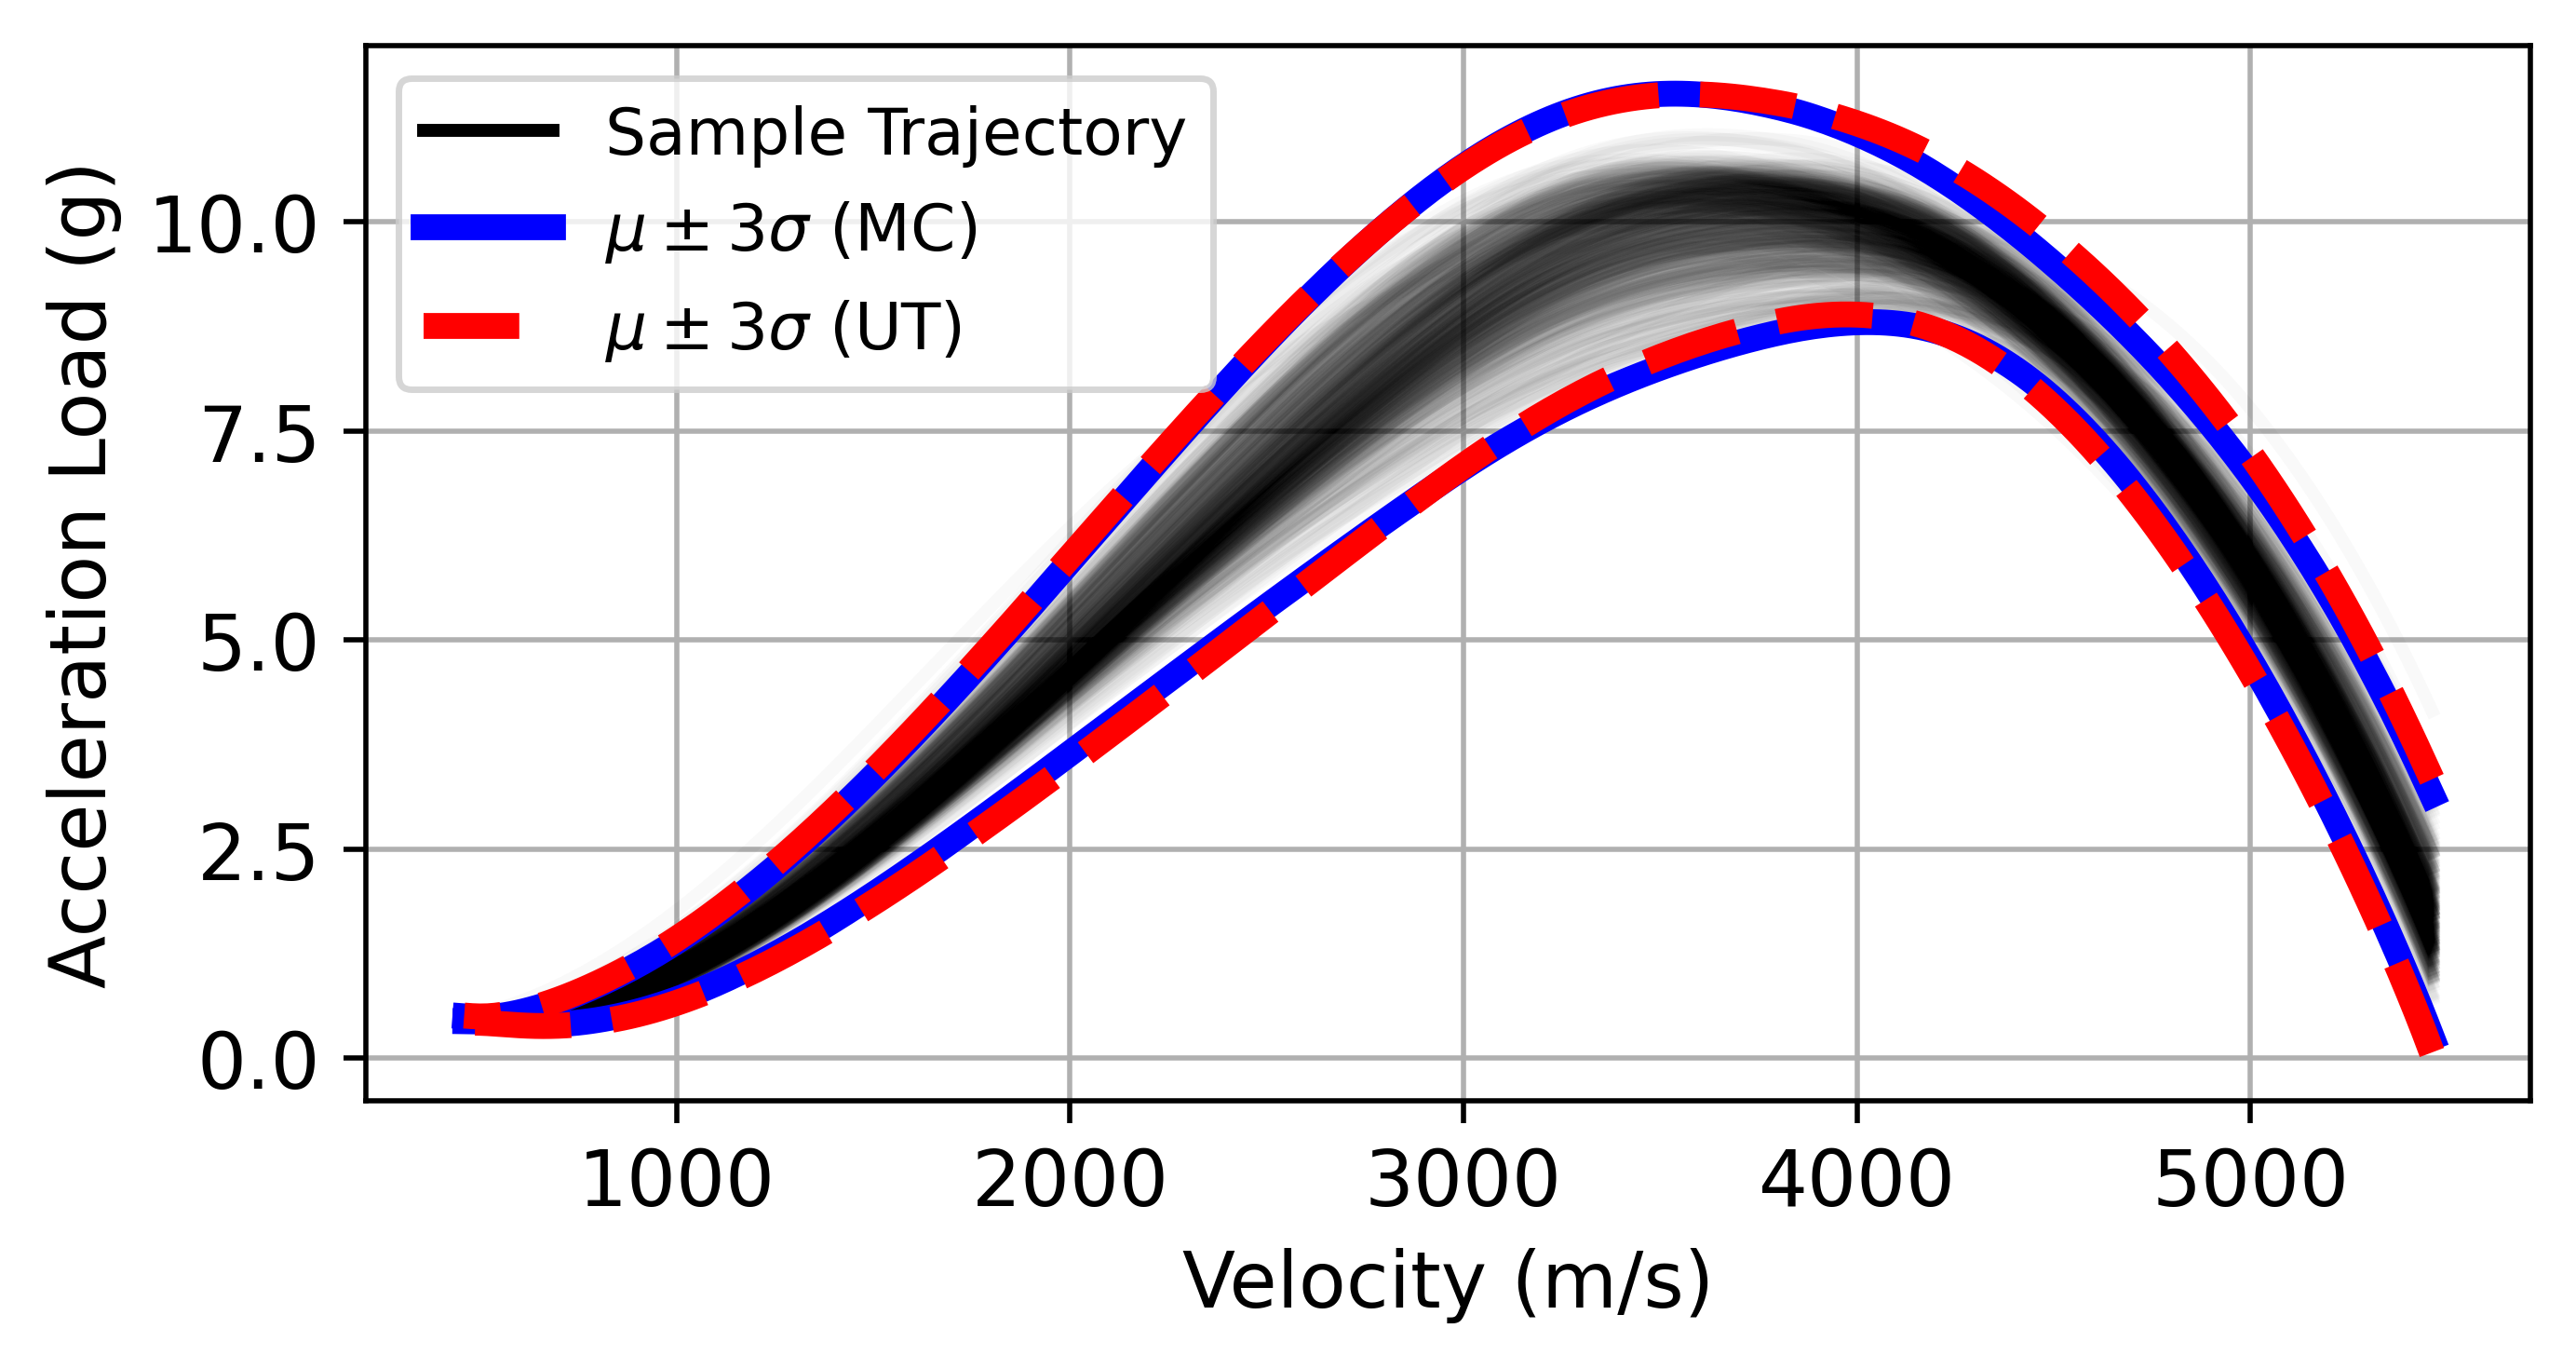
\includegraphics[width=0.75\textwidth]{../PropellantOptimalJournal/ddp/python/Acceleration}
	\caption{Acceleration load vs velocity for 500 sample trajectories with Monte Carlo- and UT-estimated 3$\sigma$ bounds.}
	\label{fig_mc_accel}
\end{figure}
\begin{figure}[h!]
	\centering
	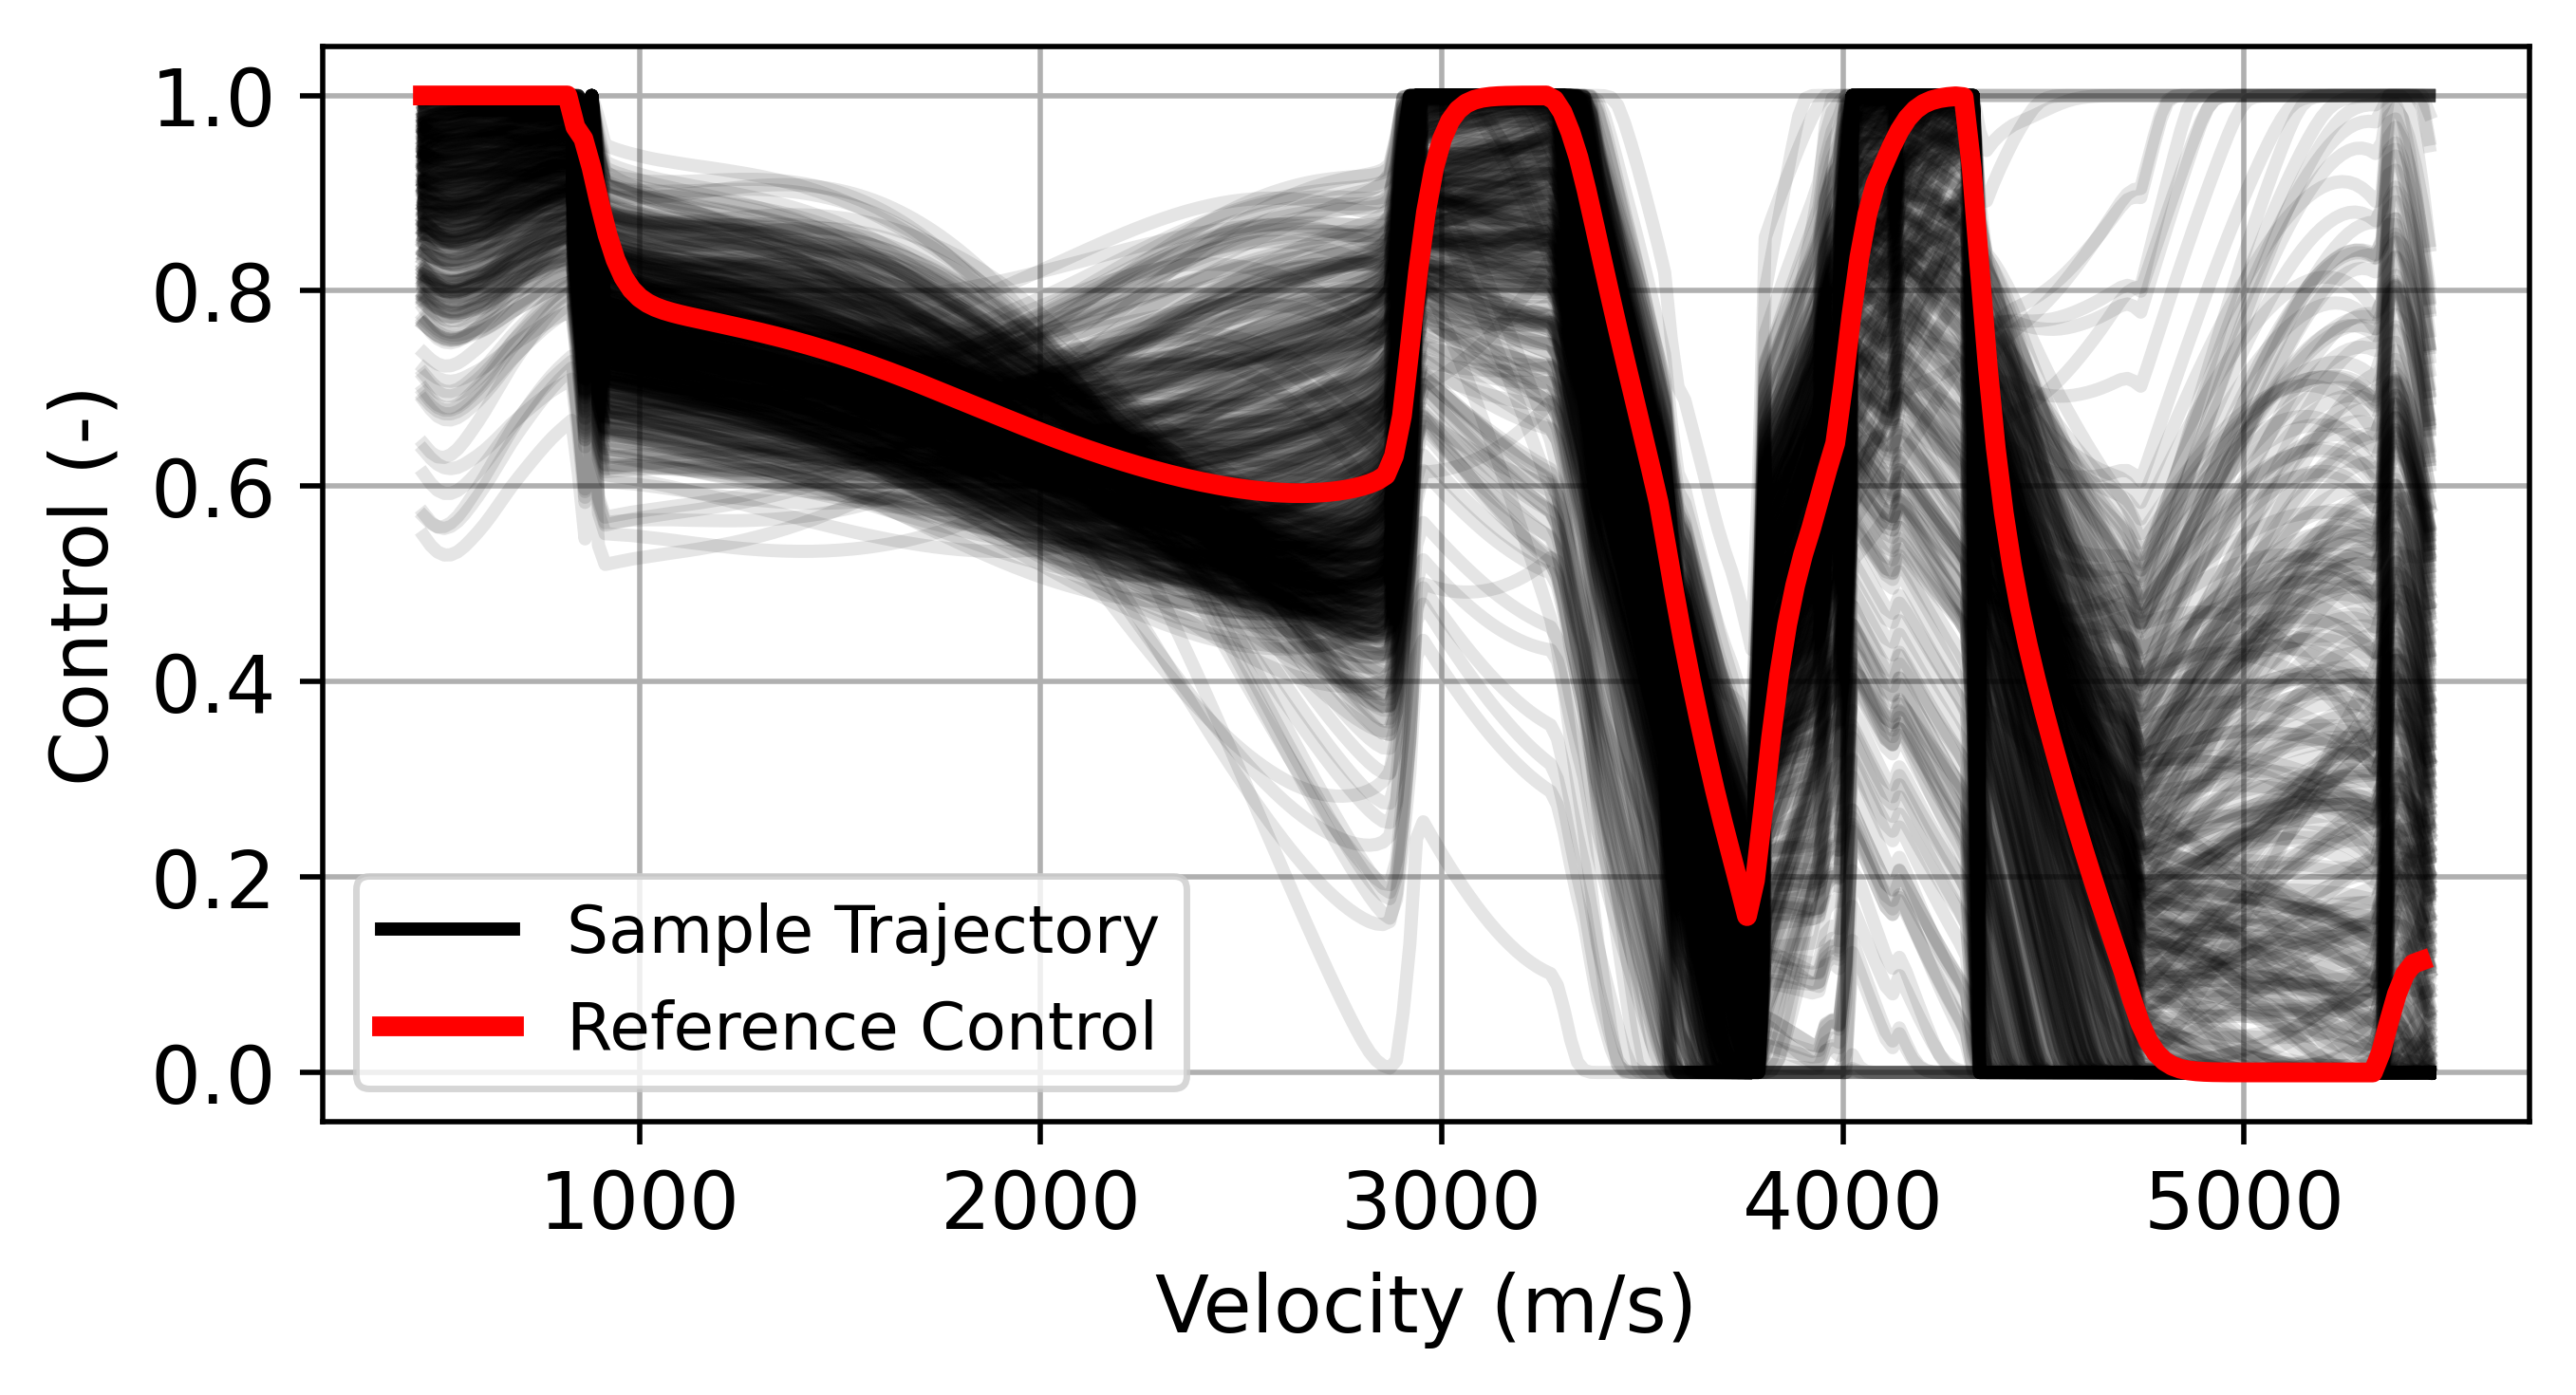
\includegraphics[width=0.75\textwidth]{../PropellantOptimalJournal/ddp/python/Control}
	\caption{The reference control and 500 sample trajectories.}
	\label{fig_mc_control}
\end{figure}
%Reoptimization of the gains resulted in reduction in the 3$\sigma$ range error from 2.5 km to 1.8 km.

% Statistics comparison 
Table~\ref{table_mc} compares statistics estimated with the unscented transform and Monte Carlo simulation. The reference trajectory and constant gains are quite effective, with the Monte Carlo 3$ \sigma $ range error under 2 km, despite small UT-estimation errors. This is achieved in part due to the reoptimization of the gains. This result is further strengthened by comparison with the performance of the unguided vehicle, which we recall was 3$\sigma_s = 80$ km. This is very nearly a 98\% reduction in 3$\sigma$ range error at a cost of 630 meters in 3$\sigma$-low altitude, again compared to the unguided statistics.
Relative to the Monte Carlo results, the UT overestimates the mean altitude by 100 m, the low altitude by 40 m, and underestimates the 3$\sigma $ range error by 700 m, or nearly 40\%. Because the mean trajectory is used as the reference, the UT-estimated mean error is always zero.

Figures~\ref{fig_mc_alt}-\ref{fig_mc_accel} show 500 sample trajectories as well as the Monte Carlo estimated 3$\sigma$ bounds, and the UT-estimated 3$\sigma$ bounds for comparison. Each of these figures demonstrates that the UT-estimated statistics closely approximate the Monte Carlo statistics. Like the terminal statistics in Table~\ref{table_mc}, the UT estimation errors do not have a consistent sign at every point along a trajectory; on some intervals the UT underestimates the 3$\sigma$ bounds, while on other intervals it overestimates them. More importantly, the magnitude of these errors remains small, confirming that the UT is an effective method of quantifying uncertainty in the optimization process. 
% Solution features 
Figure~\ref{fig_mc_alt} shows that lofting at low velocities is a key feature of the trajectories used to raise the terminal altitude. Contrary to prior studies that found range control is not effective at low velocities \cite{MSL_EDL2}, Fig.~\ref{fig_mc_range} shows the convergence of the 3$\sigma$ range errors from 25 km at $ v=1100 $ m/s to less than 2 km at the $v=460$ m/s. 
Figure~\ref{fig_mc_accel} shows the acceleration loads which never exceed 12g. If, as with MSL, a 15g limit is imposed, then this result indicates that a steeper mean entry flight path angle can be accommodated.

Figure~\ref{fig_mc_control} shows the reference control as well as the sample controls for the same 500 trajectory subset. The reference control resembles bang-bang profiles at high velocities before transitioning gradually to a full lift up orientation. There exist intervals with significant margin, particularly between 1000 m/s and 3000 m/s, as well as intervals in which the reference control and many sample controls are saturated. 
This is important because a full lift up orientation leaves no control authority for lateral guidance to manage the vehicle crossrange distance to the target.

%\section{Discussion}
SRL will land near Mars 2020 in Jezero Crater at an altitude of -2.566 km. Thus, for an additional 6 km timeline margin requirement (which may be insufficient for the heavier vehicle), a 3$\sigma$-low of 4.566 km is required. The range of altitudes achieved using the method demonstrates that, for the heavier vehicle under consideration, a constant L/D=0.28 is not sufficient to reach the required altitude. We note that although a constant 0.28 starts with more lift than the MSL profile, it ends with less.  

%Using the robust guidance as a design tool, we can quickly determine what constant (or up scaled MSL profile) L/D would be required to raise the 3$\sigma$-low altitude above 4.566. To bound this value from below, we consider $w_h=3,w_s=0$.

%However, the 3$\sigma$-low altitudes are approximately consistent with a landing at the intended elevation in Jezero Crater where Mars 2020 landed. 

%%% Local Variables: ***
%%% mode: latex ***
%%% TeX-master: "thesis.tex" ***
%%% End: ***

\chapter{Entry Guidance for SRP-Based EDL}\label{Ch:FuelOptimalPaper}
%TODO: Examine this intro, merge some of it into the actual dissertation intro and leave the rest as the intro to this chapter...
In this chapter we turn our attention away from current generation EDL architectures and consider a hypothetical future scenario. This chapter and Chapter~\ref{Ch:FuelOptimalAssessment} are based on our work in Ref.~\cite{NoyesSRP}.
Among the many considerable challenges involved in the Entry, Descent, and Landing (EDL) of a spacecraft on Mars, perhaps the greatest is the low density of the Martian atmosphere \cite{BraunMarsEDL, joel_dissertation}. At approximately one percent of the Earth's atmospheric density, current generation Mars entry vehicles are incapable of achieving sufficient deceleration to reach subsonic speeds before reaching the surface, necessitating the use of EDL technologies including supersonic parachutes and retropropulsion, both of which were utilized in safely landing MSL's Curiosity rover \cite{MSL_EDL}, and Mars 2020's Perseverance \cite{M2020_EDL}. As the mass (or ballistic coefficient) of these vehicles grows, the problem is exacerbated until safe deployment conditions for current supersonic parachutes are not reachable at altitudes high enough to provide sufficient timeline margin for subsequent EDL events \cite{BraunMarsEDL}. In such missions, supersonic retropropulsion (SRP) may be relied upon to land larger, heavier vehicles relative to the current generation of landers without the use of a parachute, and as a result powered descent will play an even more significant role in the EDL process. In this chapter and the next, the emphasis is on the interplay between the entry phase and the powered phase, and thus only these two phases are considered.

%\textbf{It might be good to talk about the two phases here.}Figure~\ref{fig_phases} shows the two-phase EDL problem under consideration. 
The challenges during the entry phase from a guidance perspective include entry state dispersions due to delivery errors, atmospheric winds and density uncertainty, aerodynamic uncertainty, and imperfect onboard state estimation, each of which contribute to the size of the landing footprint. MSL was the first Mars entry system to utilize hypersonic guidance to autonomously steer the spacecraft toward the target, which resulted in a landing footprint nearly an order of magnitude smaller than previous unguided ballistic entries \cite{BraunMarsEDL}. Mars 2020 improved upon the MSL guidance design by incorporating a range trigger~\cite{TriggerComparison2020} to deliver Perseverance to a 99\% touchdown ellipse of 7.1 km $\times$ 6.5 km. 
It is expected that a feature of SRP-based EDL is the requirement for pinpoint accuracy, defined as a sub-100 meter landing ellipse \cite{GNC_Pinpoint}. Assuming an entry guidance meets the basic requirement of delivering the vehicle to a state from which the powered guidance can achieve pinpoint landing, dispersed entry trajectories result in increased propellant requirements, rather than contribute to the landing ellipse. As a result, rather than judge an entry guidance algorithm by its landing ellipse, the propellant cost or propellant mass fraction (PMF) of the powered descent trajectory may now be considered a primary metric.

A fundamental difference of retropropulsion-based EDL from parachute-based EDL architectures, even those that utilize a vertical powered descent phase with potential for a divert maneuver beforehand, lies in the set of desirable states at the termination of the entry phase. In parachute-based EDL, the terminal entry state is constrained by safe parachute deployment conditions defined by upper and lower limits on Mach number and dynamic pressure. The constraints are often translated into constraints on altitude and velocity using a model of the Martian atmosphere. In summary, when a chute is involved, the target set for entry guidance is the parachute deployment box coupled with small downrange and crossrange errors, combined with a well-aligned heading, and no restriction on flight path angle. 

Traditionally, the primary objective of bank angle modulation during entry is range control with lateral control as a secondary objective, and guidance approaches could treat the two problems as decoupled. During the mission design phase, the downrange distance is chosen to be compatible with the parachute deployment conditions and other mission parameters such as the entry flight path angle. The target set in SRP-based EDL is in some sense much larger, but with more coupling between the state variables because, for a given powered descent guidance, the final entry state determines if pinpoint landing can be achieved, and if so, the propellant mass required. All six entry state variables contribute to the propellant cost; the optimal downrange distance and altitude at which to ignite depend on both the velocity magnitude and the flight path angle, while aligning the heading eliminates crosstrack flight during powered descent. 

% Altering the objective of entry guidance to shaping the trajectory for the benefit of the powered descent phase thus encourages a coupled approach. 
%For example, MSL utilized a range control phase and a heading alignment phase. Once the heading is aligned, the bank angle command will remain zero until the termination of the entry phase. Thus, unless heading alignment is initiated at the right time for zero bank angle to lead to the best termination condition, blah blah.

There exist many guidance solutions to the powered descent problem, often with a focus on propellant optimality. Classes of such algorithms include G-FOLD \cite{gfold,gfold_flighttests} and other convex optimization-based methods, polynomial-based approaches including the venerated Apollo lunar descent guidance \cite{apollo_lunar}, indirect optimal control methods \cite{PropellantOptimalAdaptiveTrigger}, and many others. 

Far less attention has been given to the role of entry guidance when followed directly by a powered descent phase, without an intermediate phase that makes use of a parachute or other decelerator. Reference~\cite{LuAdaptiveEDL} presents one approach to entry guidance in a chuteless EDL architecture. Reference~\cite{LuAdaptiveEDL} correctly identifies the potential for integrating the entry phase with the subsequent powered descent phase as an opportunity to reduce propellant consumption, and the vehicle bank angle is modulated to perform range control, utilizing a bank profile that is linear-in-energy with one free parameter. Lateral logic to determine bank reversals is applied separately after solving for the bank angle magnitude. Reference~\cite{EDL_AllProp} investigated an alternative EDL scheme in which aerodynamic control during entry is foregone in favor of hypersonic retropropulsion, essentially eliminating the entry phase. 

The proposed entry guidance for SRP-based EDL is designed to deliver the vehicle to a target set of states from which pinpoint landing can be achieved in the subsequent powered descent phase. Of the reachable states in the target set, entry guidance steers the vehicle to the one that will require the minimum propellant mass for pinpoint landing. For the simulation testing in this paper, the target set is computed by solving optimal control problems. 
%Details of this computation are presented later. This mapping is utilized in two distinct ways. At points along a given entry trajectory, the propellant cost can be computed in order to determine the best ignition condition for that trajectory. Additionally, the bank angle profile can be modified to intersect a portion of the feasible ignition set with sufficiently low propellant cost, using the mapping.  
%If the trajectory is poor, there may be not suitable ignition point, and the bank angle profile should be modified.
The possibility of computing the powered descent controllable set to be used as a target set for an entry guidance algorithm was suggested in Ref.~\cite{SRP_ControllableSets}, wherein a procedure based on convex optimization was designed to efficiently compute it is given.

MSL triggered its parachute deployment and descent sequence using a velocity trigger \cite{MSL_EDL2}, while Mars 2020 will utilize a range trigger \cite{M2020_EDL} to dramatically decrease the size of the landing ellipse \cite{TriggerComparison2020}. A component of our approach is an onboard determination of when to trigger powered descent initiation.  In essence, the role of such a trigger is to ensure the minimum propellant ignition point is found along any entry trajectory that has at least one feasible ignition state. The theoretical developments behind one such trigger were introduced in Ref.~\cite{PropellantOptimalAdaptiveTrigger}, while Ref.~\cite{LuAdaptiveEDL} demonstrated its benefits over triggering at a fixed state variable, such as downrange, velocity, or energy.
One potential weakness of the trigger in Ref.~\cite{PropellantOptimalAdaptiveTrigger} is that it assumes a propellant optimal powered descent guidance. In theory, future Mars missions, especially those transporting humans, may very well consider a guidance algorithm with a different objective, such as prioritizing safety or even passenger comfort, as the bang-bang nature of propellant optimal powered descent solutions may not be suitable, despite the importance of limiting propellant consumption. 

Despite presenting an approach in which a prediction of the terminal entry state is available and being used to modulate the vehicle bank angle, in Ref.~\cite{LuAdaptiveEDL} only the current vehicle state is checked for triggering the powered descent initiation. Our approach to the triggering mechanism differs in that we utilize the predicted trajectory. This allows us to query the mapping from the powered descent guidance algorithm at points along the predicted trajectory to generate propellant consumption predictions.  The benefit of doing so is two-fold. Firstly, the propellant optimal ignition point along an entry trajectory can be determined for any subsequent powered descent guidance, even one that is itself not propellant optimal. Secondly, by making explicit use of these predictions in the entry guidance algorithm, the two phases become linked by more than just the onboard triggering strategy, and superior propellant performance can be achieved. 

%Additionally, as mentioned above, our proposed entry guidance approach utilizes the powered descent guidance to be employed in the subsequent phase, in order to generate predicted propellant costs along a predicted trajectory. In this approach, the bank angle is actively modulated to reduce predicted propellant consumption rather than achieve a range objective, thereby allowing the entry guidance algorithm to suitably shape the trajectory in preparation for powered descent. It is this coordinated effort that allows the proposed entry guidance to produce superior results over traditional entry guidance methods. 

%We note that Reference Fully-Propulsive Mars Atmos Strategies for High-Mass Payload Missions looked at chuteless architectures but did not utilize lifting for control, and instead employed HYPERsonic retropulsion.
\section{Entry Guidance Problem for SRP-Based EDL}
The problem under investigation in this chapter considers a two-phase EDL sequence consisting of an entry phase and a powered descent phase. The dispersions in vehicle state arising from the approach phase are modeled as delivery errors at the beginning of the EDL sequence. In the entry phase, the vehicle is guided via bank angle modulation and the vehicle state is described in spherical coordinates, as described in Chapter~\ref{Ch:Models}. In the descent phase, the vehicle is guided via supersonic retropropulsion with the equations of motion given in Cartesian coordinates. The reason for the choice of two different coordinate systems is to be consistent with the literature on each respective topic.
\begin{figure}[h!]
	\centering
	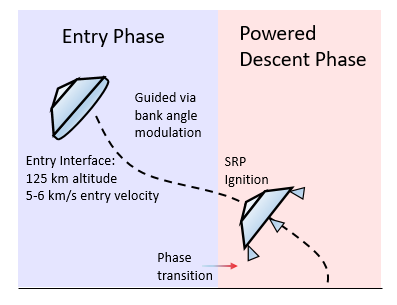
\includegraphics[width=0.5\textwidth]{../AAS20/EDLPhaseDiagram} 
	\caption{Schematic of the EDL phases.}
	\label{fig_phases}
\end{figure}

Equations~\eqref{Eq:dynamics:radius:time}-\eqref{Eq:dynamics:heading:time} will be compactly referred to as $\dot{\mathbf{x}} = f(\mathbf{x},\sigma)$ and their solution at time $t$ from a state $\mathbf{x_0}$ evolving under a bank angle profile $\sigma[0,t]$ is given by the transition map $\mathbf{x}(t) = \varphi(t;\, \mathbf{x_0},\,\sigma[0,\,t])$.

%By solving the powered descent problem on the ground over a set of possible ignition states, an entry target set may be defined that allows us to reduce the two-phase problem to a problem with only an entry phase. In this new problem, the propellant required to land is only a function of the terminal entry state, because the powered descent thrust vector profile and time of flight are no longer optimization variables. Instead, the entire powered descent trajectory is now a function of the terminal entry state.  Hence, 
The entry guidance problem is to determine the entry phase duration and a bank angle profile that will deliver the vehicle from the entry interface to the propellant-optimal point in the target set, i.e., the set from which pinpoint landing can achieved. A formal definition of the target set is given in the subsequent section.
%\begin{align}
%\min \mathrm{prop}(\mathbf{x}(t_{pd})) \label{eq_entry_ocp}\\
%&\mathbf{x}(t_0) = \mathbf{x_0} \\
%&\mathbf{x}(t_{pd}) \in \mathcal{F}_M \\
%&\dot{\mathbf{x}} = f(\mathbf{x},\sigma)
%\end{align}

\subsection{Entry Guidance Target Set}
The entry guidance target set is defined by the powered descent algorithm to be used during the descent phase, and the available propellant onboard the vehicle. The equations of motion for a point mass vehicle in powered flight in a surface fixed frame, neglecting aerodynamic forces and Coriolis effects, are
\begin{align}
&\dot{\mathbf{r}} = \mathbf{v} \label{eq_eom_srp} \\
&\dot{\mathbf{v}} = \frac{\mathbf{T}}{m} + \mathbf{g}(\mathbf{r}) \\
&\dot{m} = -\frac{||\mathbf{T}||}{I_{sp}G_0} \label{eq_eom_srp_end}
\end{align}
where $\mathbf{r}\in\mathbb{R}^3$ is the position vector of the vehicle, $\mathbf{v}\in\mathbb{R}^3$ is the velocity vector of the vehicle, $m$ is its mass, $\mathbf{T}\in\mathbb{R}^3$ is the thrust vector of the vehicle, $\mathbf{g}\in\mathbb{R}^3$ is the gravitational acceleration vector, $I_{sp}$ is the specific impulse of the rocket engine, assumed to be constant, and $G_0$ is the gravitational acceleration magnitude at the surface of the Earth. The full powered descent state vector in $\mathbb{R}^7$ comprises the position, velocity, and mass. 

%The powered descent problem considered herein is to determine the optimal thrust magnitude and direction, as well the optimal time of flight, that solve the pinpoint landing boundary value problem comprising the equations of motion with prescribed initial and final conditions, while subject to constraints on the available thrust. 
Any powered descent algorithm capable of meeting the pinpoint landing requirement may be considered. To eschew the choice of a specific algorithm in this work, the powered descent problem is posed as the optimal control problem
\begin{align}
\max \;m(t_f) \label{eq_srp_ocp}\\
&\mathbf{r}(t_0) = \mathbf{r_0} \\
&\mathbf{v}(t_0) = \mathbf{v_0} \\
&m(t_0) = m_0\\
&\mathbf{r}(t_f) = [0,\, 0,\, z_{\mathrm{target}}] \\
&\mathbf{v}(t_f) = [0,\, 0,\, \dot{z}_{\mathrm{target}}] \\
0 <\,\, &T_{\min} \le ||\mathbf{T}(t)|| \le T_{\max}
\end{align}
%together with the dynamics Eq.~\ref{eq_eom_srp}-\ref{eq_eom_srp_end},
where the final time $t_f$ is free, $T_{\min}$ and $ T_{\max} $ are constant bounds on the available thrust, and $z_{\mathrm{target}}$ and $\dot{z}_{\mathrm{target}}$ are the desired altitude and vertical velocity at the end of the descent phase. For a fixed initial mass, maximizing the final mass is equivalent to minimizing the propellant use. Formulated as such, the optimal control problem can be viewed as a function $\mathrm{OCP}(\cdot)$ that maps an initial condition, i.e., ignition state, to a propellant cost. 
The set of initial states for which the optimal control problem has a feasible solution includes regions that are not of interest. Examples include states with initial altitudes very low to the ground, initial velocities much higher than those reachable by the entry vehicle before impacting the surface, and initial distances very far from the target, or having already overshot the target. Denoting $\mathbf{r} = [x,y,z]^T$, the set of feasible solutions is restricted to a region of interest by defining a set of constraints
\begin{equation}
c_i(\mathbf{x})\le 0\:\; \mathrm{for}\,\;i=\{1,2,3,4\}\\
\end{equation} where 
\begin{align}
\mathbf{c}(\mathbf{x}) = \left[ \begin{array}{lc}
        x^2 + y^2 - d^2_{\max}\\
        d^2_{\min} - x^2 - y^2\\
        z_{\mathrm{target}} + z_{\min} - z \\
        ||\textbf{v}|| - v_{\max}
        \end{array} \right]\label{eq_constraints} 
\end{align} 
%to be applied $c_i(\mathbf{x}) \le0\;\mathrm{for}\,i=1,...,4$, and where 
and $[d_{\min},\,d_{\max}]$ are the minimum and maximum distance to the target, $z_{\min}$ is the minimum altitude, and $v_{\max}$ is the upper bound on velocity. 
%Let the controllable set, $\mathcal{C}$, be defined as the set of initial states for which there exists a thrust control function that leads the vehicle to the specified final state. We assume that $\mathcal{C}$, and the set of initial states for which the optimal control problem has a solution, are the same. 
The set of all initial state vectors for which the solution to the optimal control problem is feasible and the propellant required by the solution is less than some prescribed maximum $ M $, and satisfying these constraints is 
\begin{align}
\mathcal{F}_{M} = \left\{\mathbf{x}\,|\, \max_{i={1,...,4}}c_i(\mathbf{x})\le 0\,\,\mathrm{and}\,\,\mathrm{OCP}(\mathbf{x}) \le M \right\},
\end{align}
and is the set targeted by the entry guidance algorithm. Although the set is used an entry guidance target, it is defined in terms powered descent state variables. As the initial T/W ratio of the vehicle increases, $\mathcal{F}_{M}$ contracts. This is because, for a fixed $I_{sp}$ and $T_{\min}$, increasing thrust will increase the mass flow rate and decrease the maximum time of powered flight, which naturally decreases the distance from the target the vehicle can fly. The effect is that higher T/W places more stringent requirements on the entry guidance target set unless additional propellant is added, or the value of $I_{sp}$ or $T_{\min}$ changes.

Given an entry state and target position, the corresponding descent state is determined by assuming the current heading $\psi$ defines the downrange direction. The downrange and crossrange distances to the target are computed via spherical trigonometry \cite{joel_dissertation}
\begin{align}
d &= \cos^{-1}\left(\sin\phi\sin\phi_{\mathrm{target}} +\cos\phi\cos\phi_{\mathrm{target}}\cos(\theta_{\mathrm{target}}-\theta)        \right) \\
\Psi &= \pi/2 - \mathrm{sign}(\theta_{\mathrm{target}}-\theta) \cos^{-1}\left(\frac{\sin\phi_{\mathrm{target}}-\sin\phi\cos d}{\cos\phi\sin d}  \right) \\
c &= \sin^{-1}\left(\sin d\,\sin(\psi-\Psi))\right)
\end{align}
\begin{align}
DR &= R_p\cos^{-1}\left(\frac{\cos d}{\cos c}\right)\\
CR &= R_pc
\end{align}
where $R_p$ is the planet radius. 
%The altitude above the target is computed by subtracting the target altitude $z_{\mathrm{target}}$ from the current altitude $h = R-R_p$ and 
The full powered descent state vector in terms of the entry state variables is $[DR,\, |CR|,\, R-R_P,\, -V\cos\gamma,\, 0,\, V\sin\gamma,\, m_0]^T$. Because the downrange direction is defined by the current heading angle, the crossrange velocity is always zero. Under the assumed dynamics and zero crossrange velocity, the sign of the crossrange to the target does not affect the propellant cost, and its absolute value is used.

By using a downrange-crossrange coordinate system based on the current heading, an infinite number of entry states map to the same SRP state as a result of this surjective transformation. Intuitively, this reflects the rotational symmetry of the problem around the $z$-axis, stemming from the fact that states $ x $ and $ y $ have identical dynamics. For the powered descent problem as posed, any initial state $[ x,\, y,\, z,\, \dot{x},\, \dot{y},\, \dot{z},\, m]$ such that $(z, \dot{z}, m)$ are fixed and 
\begin{align}
x^2 &+ y^2 = p^2 \\
\dot{x}^2 &+ \dot{y}^2 = v^2 \\
\psi &= \tan^{-1}(y/x) \\
\dot{x} &= -v\cos\psi \\
\dot{y} &= -v\sin\psi \\
\end{align}
lies along an iso-propellant contour defined by the horizontal distance and velocity magnitudes, $p$ and $v$. An alternative mapping from entry states to powered descent states is to convert the entry state and target to Cartesian coordinates and subtract them. Although this is a feasible option, it is not preferable because it would result that every entry state maps to a unique SRP state. This is undesirable because it requires a larger table of solutions encompassing all the possible Cartesian states.

\section{Proposed Entry Guidance}
%Components of entry guidance: 
%Bank angle parametrization
%SRP guidance -> N-D table of propellant costs -> Required to determine both hand off state and params to get there 
%Onboard determination of ``handoff" i.e. transition from Entry phase to SRP phase 
%TODO: Minimum propellant set may be more appropriate - don't know that the set is a single point
The objective is to deliver the vehicle to the minimum propellant ignition point in the feasible subset $\mathcal{F}_M$ that is reachable under the chosen bank angle parametrization from the current state. This is in contrast to prescribing ad hoc rules for the terminal entry set to reduce propellant consumption, such as minimizing velocity at a certain downrange distance to the target. 
%Seeking the optimal point requires that the terminal entry state be free of such constraints, i.e., it cannot be required to lie on a manifold defined by a fixed velocity or distance from the target. 
This objective is accomplished by the guidance algorithm using a nested computational structure. At the inner level, the propellant map is used to determine the optimal ignition point along each predicted trajectory. At the outer level, the bank angle profile is optimized to find the optimal ignition state that is reachable from the current vehicle state. To mitigate the complexity of determining the bank angle function during flight, a parametrization is chosen on the ground, and its parameters are repeatedly optimized during flight. Thus, the three key components of the approach are the powered descent propellant map, the bank angle parametrization, and the onboard determination of the vehicle state at which the entry phase ends and powered descent begins.  

\begin{figure}[h!]
	\centering
	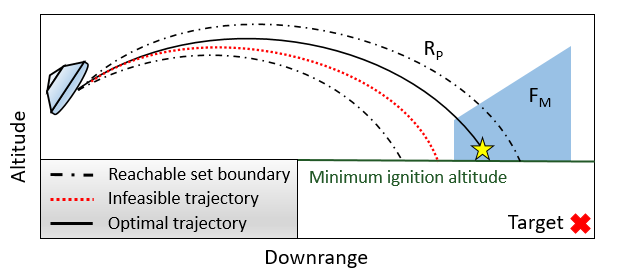
\includegraphics[width=0.8\textwidth]{../AAS20/Optimization} 
	\caption{The guidance algorithm seeks both the propellant-optimal ignition point (indicated by a star on the plot) and the trajectory whose optimal ignition point is best (indicated by the solid black line). The red, dotted trajectory is valid entry trajectory within the reachable set, but is infeasible because it does not intersect the powered descent feasible subset $\mathcal{F}_M$.}
	\label{fig_optimization}
\end{figure}

%At the core of the proposed entry phase guidance approach is an extension of the trajectory prediction to include the following powered descent phase. This allows one to alter the entry guidance objective from range control to propellant minimization. After applying several constraints to filter down the set of potential ignition states, the powered descent guidance is used to generate predictions of the propellant required from different states. The lowest among them is selected as the planned handoff condition from entry to powered descent. Further details on these constraints are given later.

%Notice that although propellant minimization is the entry guidance objective, any powered descent guidance algorithm with pinpoint landing capability may be used in the powered descent phase so long as an estimate of the propellant required is given by the algorithm, and this estimate is continuous with respect to the initial state. Thus, although in the examples of this work we have coordinated the powered descent phase to also be propellant-optimal in nature by solving the associated OCP, there exist many alternatives such as energy-optimal guidance or non-optimization based approaches such as polynomial guidance. 

%We further assume that the chosen powered descent method incorporates any necessary problem constraints, because the entry guidance algorithm does not make use of the predicted powered descent trajectory, nor does it check for satisfaction of constraints, but instead utilizes only the propellant cost associated with the powered descent trajectory. 
\subsection{Bank Angle Parametrization}
The entry phase guidance problem is intended to be solved onboard and so motivates a low-order parametrization of the bank angle profile. Parametrizing the bank angle function converts the optimal control problem into a more tractable nonlinear optimization problem. The choice of parametrization has important implications on the entry reachable set. The entry phase reachable set from an initial state $ \mathbf{x}_0$ is a tube of trajectories satisfying the equations of motion under admissible control functions 
\begin{equation*}
\mathcal{R}(\mathbf{x}_0)=\left\{\mathbf{x} \,| \,\exists\, t_f \;\mathrm{and}\; \sigma[0, t_f] \,\mathrm{with}\, \mathbf{x} = \varphi(t_f;\mathbf{x}_0,\, \sigma[0, t_f])  \right\}
\end{equation*}
and the portion of the reachable set that is of interest is its intersection with the powered descent feasible subset, i.e., $\mathcal{R} \cap \mathcal{F}_M$. Conceptually, by parametrizing the bank angle function in a particular way, we restrict the possible bank angle functions that can be generated, and as result will reduce the size of the reachable set. Let $R_P$ be the reachable set corresponding to a parametrization $ P $.
%The P-parametrized bank angle profile is a function of a finite set of parameters $P = \left\{p_1, p_2, ...,p_N \right\}$ and an associated function $h(\cdot)$ that defines the bank angle for each state, $\sigma(t) = h(P(x(t)))$.
%The dependence is to indicate closed loop nature, i.e. the values that P takes on change with the state unless flying perfectly along the optimal trajectory already 
%The P-parametrized reachable set is 
%\begin{equation*}
%\mathcal{R}(\mathbf{x}_0)=\left\{\mathbf{x} \,| \,\exists\, t_f \;\mathrm{and}\; \sigma(t)\,\forall\, t\in\,[0,t_f] \,\mathrm{with}\, \mathbf{x} = \varphi(\mathbf{x}_0; \sigma(t))  \right\}
%\end{equation*}
%$R_P(\mathbf{x}_0) =\left\{\mathbf{x}_f \,| \,\exists\, t_f \land\, P(\mathbf{x}) \,\mathrm{such\, that}\, \mathbf{x}_f = \varphi(t_f;\,\mathbf{x}_0,\, P(x(t))))  \right\} $. 
The relative size of $\mathcal{R}_P \subset \mathcal{R}$ is not the only consideration in choosing a parametrization. 
It is also desirable that $\mathcal{R}_P$ retains the propellant optimal point (or set) and neighboring region. 
%More formally, in addition to considering the effects of a parametrization on some measure of $\mathcal{R}_P\cap \mathcal{R}$, one may also consider the optimality gap, 
As a result, one might like to compare the propellant cost associated with a parametrization with the optimal solution over all parametrizations, i.e., compute
\begin{align}
\delta m = \left( \min_{x\in (\mathcal{R}\cap \mathcal{F}_M)} \mathrm{OCP}(x)\; - \min_{x\in (\mathcal{R}_P\cap \mathcal{F}_M)} \mathrm{OCP}(x) \right) \; \ge 0
\end{align}
in order to assess its quality, but this may be difficult to do. Instead, the minimum propellant costs of any two parametrizations can be compared against one another directly.  Let $\lambda$ be a measure of the volume of a state space set. Let $ P_A $ and  $ P_B $ be two different parametrizations, such that $\lambda(\mathcal{R}_{P_A}) < \lambda(\mathcal{R}_{P_B})$, and $\lambda(\mathcal{R}_{P_A}\cap \mathcal{R}) < \lambda(\mathcal{R}_{P_B}\cap \mathcal{R})$.
%but $\lambda(\mathcal{R}_{P_A}\cap \mathcal{F}_M) > \lambda(\mathcal{R}_{P_B}\cap \mathcal{F}_M)$.
Figure~\ref{fig_sets} depicts the relationship between the sets $\mathcal{F}_M,\,\mathcal{R},\,\mathcal{R}_{P_A},\,\mathrm{and}\,\mathcal{R}_{P_B}$ as well as a possible situation to demonstrate the possibility that $ \mathcal{R}_{P_A} $ is smaller than $\mathcal{R}_{P_B}$, and can reach less of $R$, yet has a smaller optimality gap than parametrization $ P_B $. 
\begin{figure}[h!]
	\centering
	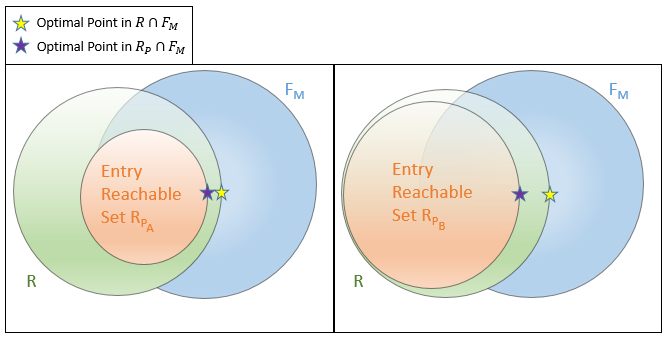
\includegraphics[width=0.9\textwidth]{../AAS20/SetDefinitions} 
	\caption{Consider two different parametrizations of the control, $ P_A $ and $ P_B $. While $ P_B $ allows the vehicle to reach more of the reachable set $\mathcal{R} $ than  $P_A$, much of $ R_{P_B}$ does not intersect $\mathcal{F}_M$. Additionally, the propellant optimal point in $ R_{P_A}$ is better than the optimal point in $ R_{P_B}$, indicated by the smaller distance between the optima, which are depicted with stars.  Note that these sets, depicted notionally as convex 2-D shapes, are actually 6-D and no claim is made about their convexity.}
	\label{fig_sets}
\end{figure}
%TODO: Better describe the stars? 
%Despite $ R_{P_B} $ being a larger set encompassing more of the true reachable set $R$, the intersection $R_{P_A}\cap \mathcal{F}_M$ is ``larger" than $R_{P_B}\cap \mathcal{F}_M$ and more importantly $ R_{P_A} $ encompasses a key subset of $ R $ – the region near the optimum. The difference between the two different optima is the sub-optimality gap imposed by the chosen parametrization.

The commanded bank angle profile considered here is a constant bank angle magnitude $\sigma_c$ with one bank reversal at a velocity $v_r$ and the current velocity $V$ is used as the independent variable in place of time,
\begin{equation}
\sigma(V; \sigma_c, \,v_r) = \left\{
\begin{array}{ll}
\sigma_c & V\geq v_r \\
-\sigma_c & V < v_r
\end{array} 
\right. .
\end{equation}
These commands are fed to a rate limiter to approximate the nature of a reaction control system tracking the commands. Because the profile includes a reversal, it offers a means to control lateral motion. 

The parametrization remains the same after the reversal, but the guidance continues to update the parameter values. By setting the lower bound on $v_r$ to be less than the ignition velocity during optimization, or greater than the current velocity, there exists the possibility to have one or no reversal planned at each update. This allows for as many reversals as there are optimization updates, but in simulations there will only be one or two reversals unless significant perturbations to the vehicle's planned heading occur after the first reversal. If an additional reversal is desired to eliminate large crossrange excursions, the parametrization is easily amended to accommodate one. A second reversal can be placed at a fixed velocity, and, exactly as the algorithm is currently applied, the first reversal timing is optimized until the reversal has been completed. Then, the second reversal is treated as the new optimization variable in addition to the bank angle magnitude. Such a ``one-at-a-time" strategy was put forth in Ref.~\cite{GuangfeiReplanning}. The result is, instead of one reversal with occasionally a second, all trajectories will feature two reversals with potential for a third. 

For comparison, we also consider a second parametrization of the form 
\begin{equation}
\sigma(V; \,v_1, \,v_2) = \left\{
\begin{array}{ll}
\;\;90^{\circ} & V\geq v_1 \\
-90^{\circ} & v_2 < V < v_1 \\
\;\;0^{\circ} & V \le v_2
\end{array} 
\right.
\end{equation}
where the two parameters $v_1,\, v_2$ such that $v_1 > v_2$ dictate the timing of the bank reversals, and the bank angle magnitudes are fixed.

\begin{figure}[h!]
		\centering
		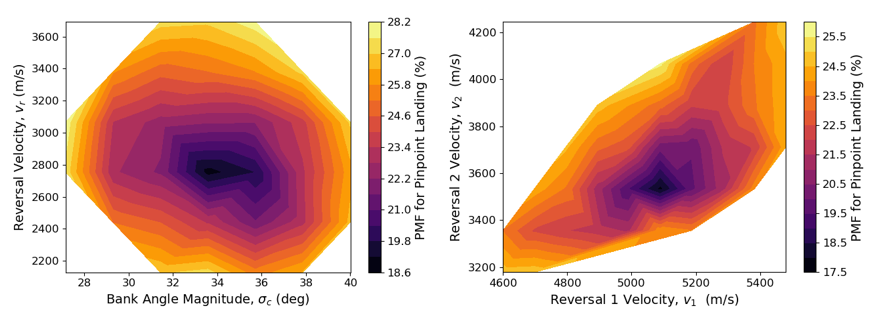
\includegraphics[width=1\textwidth]{../AAS20/ObjectiveContours} 
		\caption{Example contours of the propellant cost of pinpoint landing using two different parametrizations: a constant bank angle with one reversal, and a profile with two reversal velocities. Not only does the choice affect the propellant contours, but the reachable set is quite different as well. The downrange targeted in the constant profile is 700 km and is not reachable by the second parametrization, which instead targets 625 km. }
		\label{fig_objective_contour}
\end{figure}
%The entry guidance requires that the chosen powered descent guidance approach admits continuous propellant requirements for continuous ignition states to a fixed target. Atmospheric entry dynamics are smooth for smooth bank angle inputs and we thus expect that even when optimizing the ignition condition along a trajectory rather than use a fixed state variable such as velocity or energy, the objective function should be well-behaved and amenable to optimization. 
One key question when optimizing the parameters of the bank angle profile is whether there exist several isolated minima, or only a single global minimizer. 
Evaluating the objective function for a grid of the parameters defining the bank profile in each parametrization yields Figure~\ref{fig_objective_contour}, and indicates the objective function is likely convex, with steep gradients away from the optimum. From this, and repeated optimizations at various possible points, there is always a clear optimum.  The right plot of Figure~\ref{fig_objective_contour} shows that the two reversal parameters are significantly more coupled than the constant bank magnitude parametrization. This makes sense, as each reversal has a strong impact on the final heading, while in the constant bank parametrization, the bank magnitude has a much weaker affect on the heading than the reversal velocity. Clearly the choice of parametrization affects not only the shape of these contours, but also the minimum PMF achievable, as the second parametrization has a superior optimum. Note, however, that due to the difference in reachable set between the two parametrizations, the optimal downrange distance from the entry interface is different. For simplicity, the constant parametrization is adopted for the results in this paper. A more detailed analysis of the choice of parametrization is left for future work.

The shape of these objective functions indicates that gradient-based methods should be effective in determining the optimal profile parameters, however, determining the gradient of the objective function with respect to the switching velocity is generally difficult. As a result, derivative-free methods are preferred for this application. Powell's conjugate direction method \cite{PowellsMethod} is used in all of the examples herein. It is effective because for the chosen parametrization, the contours are nearly independent, so 1-D searches over each bounded parameter can very quickly locate the optimum. 

\subsection{Powered Descent Propellant Mapping}
By repeatedly solving the powered descent optimal control problem, Eq.~\ref{eq_srp_ocp}, for different ignition states, a pointwise approximation of a subset of the pinpoint landing feasible set $\mathcal{F}_M$ is computed via sampling. The full descent state vector is 7-D, but with two degenerate dimensions: the crossrange velocity, which is always zero by definition, and the initial mass, which is assumed to be fixed. A consequence of the dimensionality of the state space is a requirement to compute a large number of solutions -  16,807 solutions are required to span each of the remaining 5 dimensions with only 7 points. From sampled solutions we construct an approximation of the propellant costs for states in $\mathcal{F}_M$. Sampling is applicable irrespective of the powered descent algorithm to be used; for the problem of constrained propellant-optimal solutions, there exist significantly more efficient methods of computing the set $\mathcal{F}_M$ and the associated propellant cost, such as the convex optimization-based approach detailed in Ref.~\cite{SRP_ControllableSets}.

This mapping may be stored and interpolated in a variety of ways. Neural networks and other machine learning approaches were considered for their universal function approximation property. However, upon examination of the shape of the 5-D space together with numerical validation using additional OCP sample solutions, piecewise-linear 5-D interpolation was chosen to approximate the propellant mapping.
%The set of initial states over which to solve the OCP is computed by Latin Hypercube Sampling. After applying the constraints Eq~\ref{eq_constraints}, the OCP is solved for the remaining states. The model is constructed 
%TODO: Note (as Mease mentioned) that because the table is defined in SRP coordinates, it implicitly exploits the rotational symmetry as well 
%TODO: Iterative scheme
%TODO: Note the approximation is enabling, allowing MANY srp problems to be "solved" onboard
%, allowing the use of 5-D interpolation rather than 6-D. The absolute value of the crossrange distance is used because this gives a denser table of tabulated solutions by exploiting symmetry resulting from the zero crossrange velocity. 

\subsection{Trajectory Prediction and Powered Descent Ignition}
Once the bank angle parametrization is specified, the estimated entry state is integrated numerically to generate a prediction of the remaining unpowered entry trajectory. The components of the constraint vector Eq.~\ref{eq_constraints} used in the definition of $\mathcal{F}_M$ are then applied to the predicted trajectory to determine the interval that should be checked for the propellant-optimal transition to powered descent. These constraints greatly reduce the number of calls to the descent guidance propellant mapping required to find the optimum. As a reminder, these constraints include an upper bound on velocity corresponding to the maximum achievable deceleration with the available propellant, a minimum ignition altitude required for safe powered descent and subsequent EDL operations, and a maximum distance to the target, again related to the available propellant. Figure~\ref{fig_ignition} depicts this process including a portion of the trajectory already flown, the entry flight prediction, constraints, pinpoint landing target, and predicted optimal ignition point. 

Once the constraints have been applied, 1-D optimization is applied to the remaining trajectory interval, indicated by the dash black line, by viewing the fixed trajectory as a function of some independent variable. Our implementation uses velocity as the independent variable over which to search, but time or distance are also possibilities. 1-D optimization is used to very quickly locate the optimum, rather than determine the solution by brute force by checking all of the remaining points. Once the solution is determined, the commanded bank angle sign and magnitude are computed as a function of the vehicle estimated velocity, and are then sent to the control system.
%The numerical integration of the entry state is carried out using downrange distance to the target as the independent variable. Using range to go as the independent variable allows the terminal integration condition to be zero, independent of the problem specifics, with very little wasted integration time since the optimal ignition state is generally close to the target. 
%This has several advantages over common alternatives. First, although energy or velocity could be used, a sufficiently low choice of the terminal value must be made, but any time spent integrating below the reachable set of the vehicle is wasted, and the choice is problem/vehicle specific. Altitude would also be a natural choice since the minimum ignition altitude would serve as the terminal integration condition, but like energy and velocity this is problem-dependent, and additionally altitude is not a strictly monotonic variable in the case of lofting trajectories.
\begin{figure}[h!]
	\centering
	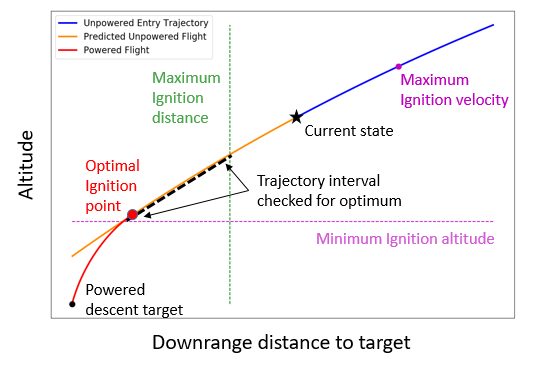
\includegraphics[width=0.7\textwidth]{../AAS20/H_Vs_S} 
	\caption{Only the interval of the predicted entry trajectory satisfying constraints on velocity, altitude, and distance to the target are searched for the propellant-optimal ignition state.}
	\label{fig_ignition}
\end{figure}


%%% Local Variables: ***
%%% mode: latex ***
%%% TeX-master: "thesis.tex" ***
%%% End: ***

\chapter{Assessment of Entry Guidance for SRP-Based EDL}\label{Ch:FuelOptimalAssessment}
In order to characterize the behavior and performance of the propellant optimal entry guidance algorithm presented in Chapter~\ref{Ch:FuelOptimalPaper}, simulations are conducted under various circumstances. In all examples, the vehicle under consideration has a nominal $L/D=0.24$, and a ballistic coefficient of $310\, \mathrm{kg/m^2}$, approximately double that of Mars 2020. The vehicle's propulsion model includes an initial $ T/W $ of 4 with a constant $ I_{sp} = 290$ s, and $T_{\min}=0.5T_{\max}$. These parameters are summarized in Table~\ref{table_model_params}.
\begin{table}[h!]
	\centering
	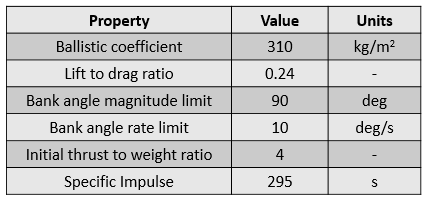
\includegraphics[width=0.6\textwidth]{../AAS20/ParamTable} 
	\caption{Model parameters used in all simulation results presented.}
	\label{table_model_params}
\end{table}
The site targeted at the termination of the descent phase is 700 km downrange with $z_{\mathrm{target}}=\dot{z}_{\mathrm{target}}=0$. 
%The entry flight path angle in all examples is $ -15.75^\circ $. The vehicle's bank angle rate is limited to $10 ^{\circ}/s$. 
Performance is evaluated using the propellant mass fraction (PMF), the portion of the vehicle that is propellant, as the primary metric. The bounds used in the constraints Eq.~\ref{eq_constraints} are $z_{\min} = 3$ km, $[d_{\min},\,d_{\max}] = [0, 25]\,$ km, $v_{\max} = 700 $ m/s. The entry phase terminates at the ignition velocity last predicted by the entry guidance algorithm.

\subsection{Sensitivity Analysis}
The performance of the algorithm is first investigated in a series of one-dimensional sensitivities to parametric uncertainties, including lift and drag coefficients, and two forms of density uncertainty. For this section, the atmospheric density is modeled as 
\begin{align}
\rho = \rho_0\mathrm{e}^{-\frac{R-R_P}{h_s}}
\end{align}
where $\rho_0 = 0.0158 \,\mathrm{kg/m}^3$ is the density at the surface and $h_s = 9354.5$ m is the scale height. Uncertainty is modeled in each of these quantities. Variations in $\rho_0$ correspond to constant percentage shift at all altitudes, while variations in the scale height alter the density's gradient with respect to altitude, $\dfrac{\partial\rho}{\partial h} = -\dfrac{\rho}{h_s}$. The guidance algorithm is called at four fixed velocities, $5500, 4000, 2000,$ and $1000$ m/s.
%Entry state dispersions are also examined. 

Due to its reliance on predictions, the algorithm is susceptible to model uncertainty. Reference~\cite{predictor_corrector_analysis} examined the performance of predictive algorithms in the presence of such uncertainties and found, like Ref.~\cite{lu2014entry}, that model adaptation during flight is essential to good performance in the presence of such parametric uncertainty. In the simulations presented, trajectory predictions are made aerodynamic accelerations scaled ratios of current sensed accelerations to modeled accelerations, $L/L_{model}$ and $ D/D_{model} $. Because the first three perturbations result in constant ratios of $L/L_{model}$ and $ D/D_{model} $, the predictions will match the simulated environment, and the predicted propellant consumption and ignition state should not vary significantly with each call to the entry guidance algorithm. In contrast, the scale height uncertainty will result in aerodynamic ratios that vary with altitude, causing error in the predictions due to their inability to account for unknown future variations. Thus it is expected to see greater variation in the predicted propellant required as well as the predicted ignition state. This behavior is exhibited in Fig.~\ref{fig_parametric_updates}.
\begin{figure}[h!]
	\centering
	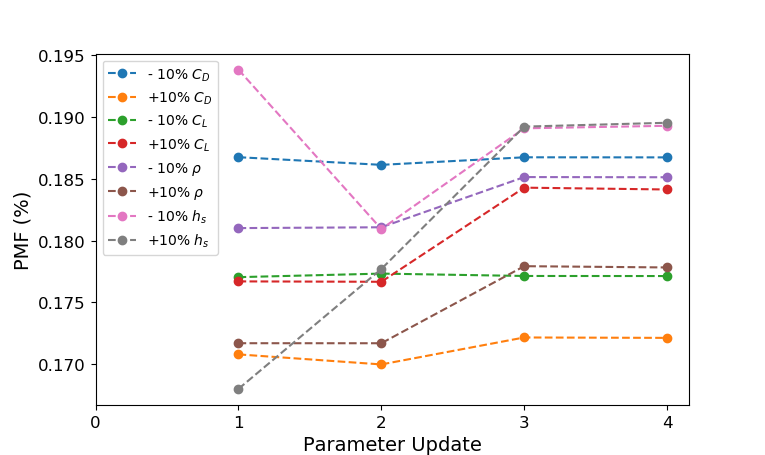
\includegraphics[width=0.7\textwidth]{../AAS20/ParameterUpdates} 
	\caption{The predicted PMF and associated ignition state may change each time the guidance algorithm is called. The solutions are less volatile when the discrepancy between the model predictions and the simulated environment is small. Larger variations in the solution due to variations in $h_s$ are expected since they result in unknown future density variations.}
	\label{fig_parametric_updates}
\end{figure}
\begin{table}[h!]
	\centering
	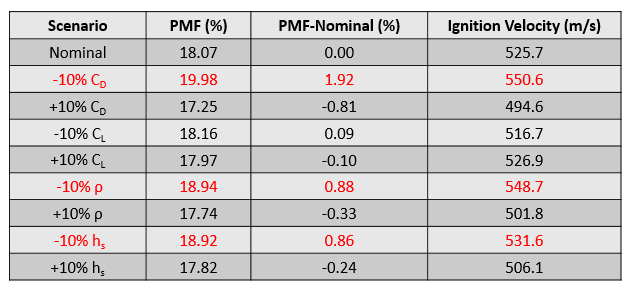
\includegraphics[width=0.75\textwidth]{../AAS20/ParametricSensitivityTable} 
	\caption{A summary of PMFs for a series of $\pm10\%$ uncertainties compared to a nominal scenario with no uncertainty. Scenarios with significant increases in PMF relative to the nominal scenario have been highlighted.}
	\label{table_parametric}
\end{table}
\begin{table}[h!]
	\centering
	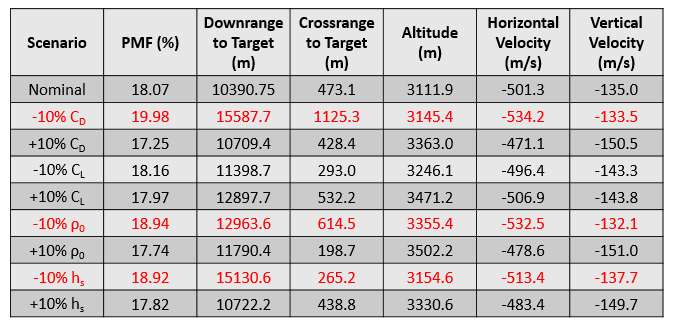
\includegraphics[width=0.8\textwidth]{../AAS20/ParametricSensitivityIgnitionTable} 
	\caption{A summary of the propellant-optimal ignition states for a series of $\pm10\%$ uncertainties. Optimal trajectories generally feature low crossrange, and altitudes close to the minimum altitude constraint.}
	\label{table_parametric_ignition}
\end{table}
\begin{figure}[h!]
	\centering
	\includegraphics[width=0.9\textwidth]{../AAS20/SensitivityBankProfiles} 
	\caption{The bank angle profiles for a series of 1-D parametric sensitivities. Despite their similar effect on drag, the controller deals with $\pm C_D$ quite differently than $\pm \rho$.}
	\label{fig_parametric_bank}
\end{figure}

Figure~\ref{fig_parametric_bank} shows the resulting bank angle profiles. Due to their similar effect on the vehicle L/D ratio, the perturbations pairs  ($ +C_D $, $ -C_L $) and ($ -C_D $, $ +C_L $) result in essentially the same update to the bank angle magnitude. The lift dispersed cases essentially fly identical altitude-velocity profiles but have slightly different reversal velocities due to the impact of lift on lateral motion. 

Table~\ref{table_parametric} summarizes the PMF for each scenario and compares them to the nominal scenario, while Table~\ref{table_parametric_ignition} gives the corresponding propellant-optimal ignition states. Several trends are noticeable. The three scenarios with the highest PMF all involve lower than nominal drag acting on the vehicle, leading to higher ignition velocities and less favorable ignition states. Although the $-10\%\, \rho_0$ case features the same decrease in drag as $-10\%\,C_D$, it also preserves the $L/D$ ratio. Unlike the drag coefficient variations, the lift coefficient variations produced very little change in PMF.
There is a noticeable asymmetry present in each of the dispersions that affects drag: the minus variation, or ``low drag" scenario, requires a greater increase in PMF than is saved in the positive variation. Note that a constant $-10\%$ variation in drag (from any source) over the entire trajectory is a substantial perturbation that is challenging to overcome in the already thin atmosphere. Despite this, the additional PMF required relative to the nominal scenario is modest.

All of the trajectories feature lofting near the end of the entry phase (not shown), and the terminal altitude is almost always very close to the minimum altitude constraint. Since altitude decreases monotonically with velocity after lofting, this allows the vehicle to decelerate for as long as possible, reducing the velocity that must be nulled by SRP. Scenarios in which the optimal ignition occurs higher indicate some other constraint is active, such as overshooting the optimal downrange distance at which to ignite. Although there is no separate guidance logic for heading alignment, it is clear from the small crossrange values in Table~\ref{table_parametric_ignition} that by targeting the optimal point in $\mathcal{F}_M$, the vehicle heading is aligned prior to ignition. 

% For a fixed ground target, a wide range of entry flight path angles (EFPAs) and entry heading errors can be accommodated by the entry guidance algorithm. Figure~\ref{fig_sweep} is an example that demonstrates the propellant cost is approximately invariant with respect to entry azimuth errors and varies weakly with EFPA, about 200 kg of propellant over $1.4^\circ$ of variation in EFPA. The range of acceptable EFPAs is often set by considerations such as g-load limits, or aerothermal constraints, and these results indicate such constraints can be imposed at little-to-no cost to propellant. 
%
%It is expected that a guidance algorithm that provides range control during entry to the same downrange distance over such a range of EFPAs will fly very different entry trajectories with a much greater variance in the propellant cost to decelerate the vehicle while landing at the target. This is significant because vehicle designers will allocate propellant based on $3\sigma$ or high percentile estimates, and reducing both the mean and variance means potential for landing greater payload masses. A numerical assessment to quantify these effects...
%
%\begin{figure}[h!]
%	\centering
%	\includegraphics[width=1\textwidth]{optimal_fuel} 
%	\caption{Propellant required for different entry flight path angles and heading angles.}
%	\label{fig_sweep}
%\end{figure}

\subsection{Monte Carlo Simulation}
\begin{table}[h!]
	\centering
	\includegraphics[width=0.4\textwidth]{../AAS20/DispersionTable} 
	\caption{The mean and $3\sigma$ values of the inputs used for the Monte Carlo simulation.}
	\label{table_input_dispersions}
\end{table}
\begin{figure}[h!]
	\centering
	\includegraphics[width=0.6\textwidth]{../AAS20/ignition_pmf} 
	\caption{Propellant mass fraction for the Monte Carlo samples.}
	\label{fig_mc_pmf}
\end{figure}
\begin{figure}[h!]
	\centering
	\includegraphics[width=0.6\textwidth]{../AAS20/bank_vel} 
	\caption{Bank angle profiles resulting from calls to the guidance algorithm at $ V=[5490, 4500, 3000, 2000, 1000] $ m/s.}
	\label{fig_mc_bank}
\end{figure}
\begin{figure}[h!]
	\centering
	\includegraphics[width=0.6\textwidth]{../AAS20/alt_vel_zoomed} 
	\caption{All of the trajectories feature lofting as a means to further decelerate prior to ignition.}
	\label{fig_mc_alt_vel}
\end{figure}
\begin{figure}[h!]
	\centering
	\includegraphics[width=0.6\textwidth]{../AAS20/dr_cr} 
	\caption{Downrange and crossrange flown from the entry state. Some trajectories fly significant crossranges due to the single planned bank reversal. Note that there are initial downrange errors in addition to than the initial crossrange errors, but due to the difference in scale they are not easily visible.}
	\label{fig_mc_entry_dr_cr}
\end{figure}
\begin{figure}[h!]
	\centering
	\includegraphics[width=0.7\textwidth]{../AAS20/ignition_dr_cr} 
	\caption{Downrange and crossrange to the target position. The crossrange is generally small, with 88\% under 1 km, indicating the vehicle heading is well-aligned at ignition.}
	\label{fig_mc_ignition_dr_cr}
\end{figure}
\begin{figure}[h!]
	\centering
	\includegraphics[width=0.7\textwidth]{../AAS20/ignition_alt_range} 
	\caption{The minimum altitude constraint, indicated in red, causes low energy scenarios to trigger at longer downrange distances and higher velocities, resulting in increased PMF.}
	\label{fig_mc_ignition_alt_vs_distance}
\end{figure}
\begin{figure}[h!]
	\centering
	\includegraphics[width=0.9\textwidth]{../AAS20/ignition_vz_vx} 
	\caption{Ignition velocity magnitude (left) and components (right). Lower ignition velocities tend to occur at steeper flight path angles for the chosen parametrization. The correlation between velocity and PMF is evident, but the slowest ignition point (bottom right of the right plot) is nowhere near the lowest PMF value, demonstrating the importance of other state variables in determining the PMF required.}
	\label{fig_mc_ignition_vel}
\end{figure}
A Monte Carlo of 1000 samples is conducted with entry state delivery errors and aerodynamic dispersions, listed in Table~\ref{table_input_dispersions}, and a higher fidelity atmosphere model. The atmospheric density is modeled using MarsGRAM \cite{MarsGRAM2010User}, rather than the exponential model employed specifically for the sensitivity study. 
 
Figure~\ref{fig_mc_pmf} shows the distribution of PMFs and
Figs.~\ref{fig_mc_bank}-\ref{fig_mc_entry_dr_cr} display the entry trajectories. The median PMF is 18.2 \%, and the 99 percentile is 20.1\%. From Fig.~\ref{fig_mc_alt_vel} it is evident that all of the samples feature at least a mild lofting near the end of the entry phase. 
Figure~\ref{fig_mc_bank} depicts the bank angle profiles. The chosen parametrization of the bank profile, coupled with the nature of the disturbances modeled, means that unless significant perturbation of the vehicle heading occurs after the first reversal, there will be only one reversal in total. In instances where the prediction was inaccurate and the reversal was poorly timed as a result, a late second reversal is used to correct the vehicle heading. 

Figures~\ref{fig_mc_ignition_dr_cr}-\ref{fig_mc_ignition_vel} plot the ignition states at the ignition velocity determined by the last call to the entry guidance algorithm. For the vehicle under consideration, the optimal downrange to the target is generally between 10-15 km. Nearly all samples have a crossrange distance of less than 1 km at ignition, and the maximum crossrange samples trigger with around 3.5 km crossrange to the target. As seen in Fig.~\ref{fig_mc_ignition_vel}, ignition velocities occur over a range of nearly 100 m/s. PMF and velocity at ignition are naturally correlated, but the lowest velocity ignition (the point in the bottom right of the right plot) is near the upper end of the PMF range, which shows that other state variables may yet have a strong impact on the PMF required to land.

Figure~\ref{fig_mc_ignition_alt_vs_distance} shows that altitude at ignition is consistently low, within 1-2 km of the minimum altitude constraint. This is not surprising, as after the vehicle has passed the point of lofting, the lowest velocity along an entry trajectory will occur at the minimum altitude.
% Thus, low altitude ignitions are known to be optimal when the ignition flight path angles are shallow ($\le20^{\circ}$). 
%While this is the case for propellant-optimal powered descent solutions, it may not be true generally, i.e., for an alternative powered descent guidance. Nevertheless, 
The consistently low ignition altitudes suggest a guidance strategy that triggers ignition at a fixed altitude may perform nearly as well as searching for the optimal ignition state. Doing so would eliminate the need to find the optimum ignition point along a trajectory, removing the nested computation structure, and leaving only the optimization over the parameters of the bank angle profile. An additional benefit of such a strategy is a reduction of the propellant mapping interpolation to four dimensions, requiring far fewer solutions to represent the mapping with the same accuracy. Additionally, some of the suboptimality associated with an altitude trigger would be mitigated by the vehicle flying slightly differently knowing that the ignition altitude is different. 

Reference~\cite{PropellantOptimalAdaptiveTrigger} also noted that propellant-optimal ignitions generally occur near the last feasible entry state, but submits that propellant consumption alone is not a sufficient criterion for powered descent ignition because it does not account for operational margins. We suggest alternatively that by defining the minimum altitude constraint with operational margin in mind, the entry guidance algorithm may utilize an altitude trigger and focus exclusively on propellant consumption without issue. Another possible generalization is to trigger on a fixed glideslope angle, essentially allowing the final altitude to be lower if the vehicle is also nearer to the target.

\begin{figure}[h!]
	\centering
	\includegraphics[width=0.9\textwidth]{../AAS20/min_alt_constraint} 
	\caption{The optimal placement of the target from the entry interface varies considerably with minimum entry altitude constraint has a strong impact on the geometry of the propellant optimal powered descent trajectories.}
	\label{fig_min_alt_constraint}
\end{figure} 
\begin{figure}[h!]
	\centering
	\includegraphics[width=0.9\textwidth]{../AAS20/SRP_vs_min_alt} 
	\caption{The minimum entry altitude constraint has a strong impact on the geometry of the propellant-optimal powered descent trajectories.}
	\label{fig_srp_traj}
\end{figure} 
 
 % %New stuff
The minimum altitude constraint also implications during mission design. Not only does it strongly affect the geometry of the powered descent phase, but it also affects the optimal entry trajectory length and the minimum propellant required.
 Figure~\ref{fig_min_alt_constraint} plots these quantities versus the value of the altitude constraint, while Fig.~\ref{fig_srp_traj} shows how the powered descent trajectories vary with the constraint. 
For the vehicle considered, and a constant bank angle magnitude during entry, the unconstrained optimal ignition altitude is about 1.5 km above the target. When the targeted downrange distance is free, the growth in PMF due to the constraint is modest, but the optimal entry downrange distance grows by nearly 40 km when imposing a 5 km constraint, and the propellant-optimal downrange distance from the target at ignition nearly doubles. 
 % %End New stuff
 
 
%\section{Discussion}
%An entry guidance algorithm for chuteless, retropropulsion-based entry, descent, and landing was proposed. In particular, we addressed the problem of steering an entry vehicle to a propellant-optimal ignition condition. Feasible solutions to the powered descent problem are used to define the entry guidance target set. By computing and storing a mapping from ignition states in the target set to propellant required, the entry guidance algorithm maintains a predicted ignition state that varies over time as various perturbations alter the reachable set of the vehicle. The guidance algorithm updates the bank profile in order to track the propellant-optimal reachable state.
%
%Although the role of entry guidance has always been to deliver the vehicle to favorable conditions for subsequent descent and landing phases, the use of the powered descent phase's guidance to define a target set, specifically for the purpose of reducing predicted powered descent propellant consumption, is novel. In parachute-based architectures, Mars entry guidance algorithms are generally judged on their ability to manage range errors while reaching the safe parachute deployment set. In contrast, in chuteless missions where pinpoint landing is achieved via powered descent, we posit that performance will instead be based on the required propellant to land the vehicle.
%
%In the presented approach, the transition from the entry phase to powered descent is determined onboard during the optimization of the bank angle profile, but numerical results suggest that a possible simplification of the trigger is possible with little to no increase in propellant. Using a fixed altitude trigger would remove the need to optimize the ignition point along individual trajectories, and would allow a further reduction in size of the propellant map due to the decrease in dimensionality of the possible ignition states. The approach was demonstrated using a simple parametrization. Future work will consider alternatives, such as a profile designed specifically for achieving low velocity, which will likely yield lower propellant consumption. 


%%% Local Variables: ***
%%% mode: latex ***
%%% TeX-master: "thesis.tex" ***
%%% End: ***

\chapter{Conclusions}

In linear systems subject to Gaussian uncertainties, the covariance matrix evolves independently of the mean trajectory, and must be shaped by feedback control. The natural nonlinearities of the entry problem, particularly the aerodynamic accelerations, which are quadratic in velocity and approximately exponential in altitude, result in drastically different evolution of the state covariance matrix along different trajectories through the atmosphere. This allows for the possibility of open-loop covariance shaping. Introducing a feedback control allows for even greater shaping of the state covariance as well as an additional nonlinearity - saturation. 

\section{Future Work}
Lateral guidance, and decision to change to third phase guidance, such as heading alignment or deployment position alignment \cite{GuangfeiDissertation}.
Navigational problem? Combined optimal estimation and control, also inclusion of nav error in guidance. While future missions may benefit from improved navigation algorithms and initialization, navigation errors remain an important source of error in assessing guidance performance. 

Nonlinear controller design for improved performance? 

Constrained optimization to make the EPFA optimization more useful, Gload/heating etc. 

%%% Local Variables: ***
%%% mode: latex ***
%%% TeX-master: "thesis.tex" ***
%%% End: ***

% ... and so on

% These commands fix an odd problem in which the bibliography line
% of the Table of Contents shows the wrong page number.
\clearpage
\phantomsection

% "References should be formatted in style most common in discipline",
% abbrv is only a suggestion.
\bibliographystyle{unsrt}
\bibliography{bib}

% The Thesis Manual says not to include appendix figures and tables in
% the List of Figures and Tables, respectively, so these commands from
% the caption package turn it off from this point onwards. If needed,
% it can be re-enabled later (using list=yes argument).
\captionsetup[figure]{list=no}
\captionsetup[table]{list=no}

% If you have an appendix, it should come after the references.
%\begin{appendices}
%% The original template (from Trevor) had a custom \appendix command,
% but I found it to break figure/table counters. I'm not sure how
% reliable my fix is, so I ended up reverting back to the standard
% latex version, and renaming the custom command to \myappendix.  You
% can try both and see how things work out:
% 1) Call \appendix once, and then make each appendix a \chapter
% 2) Call \myappendix once, and then make each appendix a \section.

\appendix
\chapter{Appendix Title}

% Appendix sections, subsections etc should not appear in the table of 
% contents. So set tocdepth to 0 and set it back to 2 at the end. Do 
% this for each appendix.
\addtocontents{toc}{\protect\setcounter{tocdepth}{0}}

Supplementary material goes here. See for instance Figure
\ref{fig:quote}.

\section{Lorem Ipsum}

dolor sit amet, consectetur adipisicing elit, sed do eiusmod tempor
incididunt ut labore et dolore magna aliqua. Ut enim ad minim veniam,
quis nostrud exercitation ullamco laboris nisi ut aliquip ex ea
commodo consequat. Duis aute irure dolor in reprehenderit in voluptate
velit esse cillum dolore eu fugiat nulla pariatur. Excepteur sint
occaecat cupidatat non proident, sunt in culpa qui officia deserunt
mollit anim id est laborum.

\begin{figure}
  \centering
  \begin{tabular}{l}
    ``I am glad I was up so late,\\
    \quad{}for that's the reason I was up so early.''\\
    \em \footnotesize William Shakespeare (1564-1616), British
    dramatist, poet.\\
    \em \footnotesize Cloten, in Cymbeline, act 2, sc. 3, l. 33-4.
  \end{tabular}
  \caption{A deep quote.}
  \label{fig:quote}
\end{figure}

\addtocontents{toc}{\protect\setcounter{tocdepth}{2}}

%%% Local Variables: ***
%%% mode: latex ***
%%% TeX-master: "thesis.tex" ***
%%% End: ***

%\end{appendices}

\end{document}